% ----------------------------------------------------------------------
%
%                            TFMTesis.tex
%
%----------------------------------------------------------------------
%
% Este fichero contiene el "documento maestro" del documento. Lo único
% que hace es configurar el entorno LaTeX e incluir los ficheros .tex
% que contienen cada sección.
%
%----------------------------------------------------------------------
%
% Los ficheros necesarios para este documento son:
%
%       TeXiS/* : ficheros de la plantilla TeXiS.
%       Cascaras/* : ficheros con las partes del documento que no
%          son capítulos ni apéndices (portada, agradecimientos, etc.)
%       Capitulos/*.tex : capítulos de la tesis
%       Apendices/*.tex: apéndices de la tesis
%       constantes.tex: constantes LaTeX
%       config.tex : configuración de la "compilación" del documento
%       guionado.tex : palabras con guiones
%
% Para la bibliografía, además, se necesitan:
%
%       *.bib : ficheros con la información de las referencias
%
% ---------------------------------------------------------------------

\documentclass[12pt,a4paper,twoside]{book}

%
% Definimos  el   comando  \compilaCapitulo,  que   luego  se  utiliza
% (opcionalmente) en config.tex. Quedaría  mejor si también se definiera
% en  ese fichero,  pero por  el modo  en el  que funciona  eso  no es
% posible. Puedes consultar la documentación de ese fichero para tener
% más  información. Definimos también  \compilaApendice, que  tiene el
% mismo  cometido, pero  que se  utiliza para  compilar  únicamente un
% apéndice.
%
%
% Si  queremos   compilar  solo   una  parte  del   documento  podemos
% especificar mediante  \includeonly{...} qué ficheros  son los únicos
% que queremos  que se incluyan.  Esto  es útil por  ejemplo para sólo
% compilar un capítulo.
%
% El problema es que todos aquellos  ficheros que NO estén en la lista
% NO   se  incluirán...  y   eso  también   afecta  a   ficheros  de
% la plantilla...
%
% Total,  que definimos  una constante  con los  ficheros  que siempre
% vamos a querer compilar  (aquellos relacionados con configuración) y
% luego definimos \compilaCapitulo.
\newcommand{\ficherosBasicosTeXiS}{%
TeXiS/TeXiS_pream,TeXiS/TeXiS_cab,TeXiS/TeXiS_bib,TeXiS/TeXiS_cover%
}
\newcommand{\ficherosBasicosTexto}{%
constantes,guionado,Cascaras/bibliografia,config%
}
\newcommand{\compilaCapitulo}[1]{%
\includeonly{\ficherosBasicosTeXiS,\ficherosBasicosTexto,Capitulos/#1}%
}

\newcommand{\compilaApendice}[1]{%
\includeonly{\ficherosBasicosTeXiS,\ficherosBasicosTexto,Apendices/#1}%
}

%- - - - - - - - - - - - - - - - - - - - - - - - - - - - - - - - - - -
%            Preámbulo del documento. Configuraciones varias
%- - - - - - - - - - - - - - - - - - - - - - - - - - - - - - - - - - -

% Define  el  tipo  de  compilación que  estamos  haciendo.   Contiene
% definiciones  de  constantes que  cambian  el  comportamiento de  la
% compilación. Debe incluirse antes del paquete TeXiS/TeXiS.sty
%---------------------------------------------------------------------
%
%                          config.tex
%
%---------------------------------------------------------------------
%
% Contiene la  definición de constantes  que determinan el modo  en el
% que se compilará el documento.
%
%---------------------------------------------------------------------
%
% En concreto, podemos  indicar si queremos "modo release",  en el que
% no  aparecerán  los  comentarios  (creados  mediante  \com{Texto}  o
% \comp{Texto}) ni los "por  hacer" (creados mediante \todo{Texto}), y
% sí aparecerán los índices. El modo "debug" (o mejor dicho en modo no
% "release" muestra los índices  (construirlos lleva tiempo y son poco
% útiles  salvo  para   la  versión  final),  pero  sí   el  resto  de
% anotaciones.
%
% Si se compila con LaTeX (no  con pdflatex) en modo Debug, también se
% muestran en una esquina de cada página las entradas (en el índice de
% palabras) que referencian  a dicha página (consulta TeXiS_pream.tex,
% en la parte referente a show).
%
% El soporte para  el índice de palabras en  TeXiS es embrionario, por
% lo  que no  asumas que  esto funcionará  correctamente.  Consulta la
% documentación al respecto en TeXiS_pream.tex.
%
%
% También  aquí configuramos  si queremos  o  no que  se incluyan  los
% acrónimos  en el  documento final  en la  versión release.  Para eso
% define (o no) la constante \acronimosEnRelease.
%
% Utilizando \compilaCapitulo{nombre}  podemos también especificar qué
% capítulo(s) queremos que se compilen. Si no se pone nada, se compila
% el documento  completo.  Si se pone, por  ejemplo, 01Introduccion se
% compilará únicamente el fichero Capitulos/01Introduccion.tex
%
% Para compilar varios  capítulos, se separan sus nombres  con comas y
% no se ponen espacios de separación.
%
% En realidad  la macro \compilaCapitulo  está definida en  el fichero
% principal tesis.tex.
%
%---------------------------------------------------------------------


% Comentar la línea si no se compila en modo release.
% TeXiS hará el resto.
% ¡¡¡Si cambias esto, haz un make clean antes de recompilar!!!
\def\release{1}


% Descomentar la linea si se quieren incluir los
% acrónimos en modo release (en modo debug
% no se incluirán nunca).
% ¡¡¡Si cambias esto, haz un make clean antes de recompilar!!!
%\def\acronimosEnRelease{1}


% Descomentar la línea para establecer el capítulo que queremos
% compilar

% \compilaCapitulo{01Introduccion}
% \compilaCapitulo{02EstructuraYGeneracion}
% \compilaCapitulo{03Edicion}
% \compilaCapitulo{04Imagenes}
% \compilaCapitulo{05Bibliografia}
% \compilaCapitulo{06Makefile}

% \compilaApendice{01AsiSeHizo}

% Variable local para emacs, para  que encuentre el fichero maestro de
% compilación y funcionen mejor algunas teclas rápidas de AucTeX
%%%
%%% Local Variables:
%%% mode: latex
%%% TeX-master: "./Tesis.tex"
%%% End:


% Paquete de la plantilla
\usepackage{TeXiS/TeXiS}


% Incluimos el fichero con comandos de constantes
%---------------------------------------------------------------------
%
%                          constantes.tex
%
%---------------------------------------------------------------------
%
% Fichero que  declara nuevos comandos LaTeX  sencillos realizados por
% comodidad en la escritura de determinadas palabras
%
%---------------------------------------------------------------------

%%%%%%%%%%%%%%%%%%%%%%%%%%%%%%%%%%%%%%%%%%%%%%%%%%%%%%%%%%%%%%%%%%%%%%
% Comando: 
%
%       \titulo
%
% Resultado: 
%
% Escribe el título del documento.
%%%%%%%%%%%%%%%%%%%%%%%%%%%%%%%%%%%%%%%%%%%%%%%%%%%%%%%%%%%%%%%%%%%%%%
\def\titulo{\textsc{TeXiS}: Una plantilla de \LaTeX\
  para Tesis y otros documentos}

%%%%%%%%%%%%%%%%%%%%%%%%%%%%%%%%%%%%%%%%%%%%%%%%%%%%%%%%%%%%%%%%%%%%%%
% Comando: 
%
%       \autor
%
% Resultado: 
%
% Escribe el autor del documento.
%%%%%%%%%%%%%%%%%%%%%%%%%%%%%%%%%%%%%%%%%%%%%%%%%%%%%%%%%%%%%%%%%%%%%%
\def\autor{Marco Antonio y Pedro Pablo G\'omez Mart\'in}

% Variable local para emacs, para  que encuentre el fichero maestro de
% compilación y funcionen mejor algunas teclas rápidas de AucTeX

%%%
%%% Local Variables:
%%% mode: latex
%%% TeX-master: "tesis.tex"
%%% End:


% Sacamos en el log de la compilación el copyright
%\typeout{Copyright Marco Antonio and Pedro Pablo Gomez Martin}

%
% "Metadatos" para el PDF
%
\ifpdf\hypersetup{%
    pdftitle = {\titulo},
    pdfsubject = {Plantilla de Tesis},
    pdfkeywords = {Plantilla, LaTeX, tesis, trabajo de
      investigación, trabajo de Master},
    pdfauthor = {\textcopyright\ \autor},
    pdfcreator = {\LaTeX\ con el paquete \flqq hyperref\frqq},
    pdfproducer = {pdfeTeX-0.\the\pdftexversion\pdftexrevision},
    }
    \pdfinfo{/CreationDate (\today)}
\fi


%- - - - - - - - - - - - - - - - - - - - - - - - - - - - - - - - - - -
%                        Documento
%- - - - - - - - - - - - - - - - - - - - - - - - - - - - - - - - - - -
\begin{document}

% Incluimos el  fichero de definición de guionado  de algunas palabras
% que LaTeX no ha dividido como debería
%----------------------------------------------------------------
%
%                          guionado.tex
%
%----------------------------------------------------------------
%
% Fichero con algunas divisiones de palabras que LaTeX no
% hace correctamente si no se le da alguna ayuda.
%
%----------------------------------------------------------------

\hyphenation{
% a
abs-trac-to
abs-trac-tos
abs-trac-ta
abs-trac-tas
ac-tua-do-res
a-gra-de-ci-mien-tos
ana-li-za-dor
an-te-rio-res
an-te-rior-men-te
apa-rien-cia
a-pro-pia-do
a-pro-pia-dos
a-pro-pia-da
a-pro-pia-das
a-pro-ve-cha-mien-to
a-que-llo
a-que-llos
a-que-lla
a-que-llas
a-sig-na-tu-ra
a-sig-na-tu-ras
a-so-cia-da
a-so-cia-das
a-so-cia-do
a-so-cia-dos
au-to-ma-ti-za-do
% b
batch
bi-blio-gra-fía
bi-blio-grá-fi-cas
bien
bo-rra-dor
boo-l-ean-expr
% c
ca-be-ce-ra
call-me-thod-ins-truc-tion
cas-te-lla-no
cir-cuns-tan-cia
cir-cuns-tan-cias
co-he-ren-te
co-he-ren-tes
co-he-ren-cia
co-li-bri
co-men-ta-rio
co-mer-cia-les
co-no-ci-mien-to
cons-cien-te
con-si-de-ra-ba
con-si-de-ra-mos
con-si-de-rar-se
cons-tan-te
cons-trucción
cons-tru-ye
cons-tru-ir-se
con-tro-le
co-rrec-ta-men-te
co-rres-pon-den
co-rres-pon-dien-te
co-rres-pon-dien-tes
co-ti-dia-na
co-ti-dia-no
crean
cris-ta-li-zan
cu-rri-cu-la
cu-rri-cu-lum
cu-rri-cu-lar
cu-rri-cu-la-res
% d
de-di-ca-do
de-di-ca-dos
de-di-ca-da
de-di-ca-das
de-rro-te-ro
de-rro-te-ros
de-sa-rro-llo
de-sa-rro-llos
de-sa-rro-lla-do
de-sa-rro-lla-dos
de-sa-rro-lla-da
de-sa-rro-lla-das
de-sa-rro-lla-dor
de-sa-rro-llar
des-cri-bi-re-mos
des-crip-ción
des-crip-cio-nes
des-cri-to
des-pués
de-ta-lla-do
de-ta-lla-dos
de-ta-lla-da
de-ta-lla-das
di-a-gra-ma
di-a-gra-mas
di-se-ños
dis-po-ner
dis-po-ni-bi-li-dad
do-cu-men-ta-da
do-cu-men-to
do-cu-men-tos
% e
edi-ta-do
e-du-ca-ti-vo
e-du-ca-ti-vos
e-du-ca-ti-va
e-du-ca-ti-vas
e-la-bo-ra-do
e-la-bo-ra-dos
e-la-bo-ra-da
e-la-bo-ra-das
es-co-llo
es-co-llos
es-tu-dia-do
es-tu-dia-dos
es-tu-dia-da
es-tu-dia-das
es-tu-dian-te
e-va-lua-cio-nes
e-va-lua-do-res
exis-ten-tes
exhaus-ti-va
ex-pe-rien-cia
ex-pe-rien-cias
% f
for-ma-li-za-do
% g
ge-ne-ra-ción
ge-ne-ra-dor
ge-ne-ra-do-res
ge-ne-ran
% h
he-rra-mien-ta
he-rra-mien-tas
% i
i-dio-ma
i-dio-mas
im-pres-cin-di-ble
im-pres-cin-di-bles
in-de-xa-do
in-de-xa-dos
in-de-xa-da
in-de-xa-das
in-di-vi-dual
in-fe-ren-cia
in-fe-ren-cias
in-for-ma-ti-ca
in-gre-dien-te
in-gre-dien-tes
in-me-dia-ta-men-te
ins-ta-la-do
ins-tan-cias
% j
% k
% l
len-gua-je
li-be-ra-to-rio
li-be-ra-to-rios
li-be-ra-to-ria
li-be-ra-to-rias
li-mi-ta-do
li-te-ra-rio
li-te-ra-rios
li-te-ra-ria
li-te-ra-rias
lo-tes
% m
ma-ne-ra
ma-nual
mas-que-ra-de
ma-yor
me-mo-ria
mi-nis-te-rio
mi-nis-te-rios
mo-de-lo
mo-de-los
mo-de-la-do
mo-du-la-ri-dad
mo-vi-mien-to
% n
na-tu-ral
ni-vel
nues-tro
% o
obs-tan-te
o-rien-ta-do
o-rien-ta-dos
o-rien-ta-da
o-rien-ta-das
% p
pa-ra-le-lo
pa-ra-le-la
par-ti-cu-lar
par-ti-cu-lar-men-te
pe-da-gó-gi-ca
pe-da-gó-gi-cas
pe-da-gó-gi-co
pe-da-gó-gi-cos
pe-rio-di-ci-dad
per-so-na-je
plan-te-a-mien-to
plan-te-a-mien-tos
po-si-ción
pre-fe-ren-cia
pre-fe-ren-cias
pres-cin-di-ble
pres-cin-di-bles
pri-me-ra
pro-ble-ma
pro-ble-mas
pró-xi-mo
pu-bli-ca-cio-nes
pu-bli-ca-do
% q
% r
rá-pi-da
rá-pi-do
ra-zo-na-mien-to
ra-zo-na-mien-tos
re-a-li-zan-do
re-fe-ren-cia
re-fe-ren-cias
re-fe-ren-cia-da
re-fe-ren-cian
re-le-van-tes
re-pre-sen-ta-do
re-pre-sen-ta-dos
re-pre-sen-ta-da
re-pre-sen-ta-das
re-pre-sen-tar-lo
re-qui-si-to
re-qui-si-tos
res-pon-der
res-pon-sa-ble
% s
se-pa-ra-do
si-guien-do
si-guien-te
si-guien-tes
si-guie-ron
si-mi-lar
si-mi-la-res
si-tua-ción
% t
tem-pe-ra-ments
te-ner
trans-fe-ren-cia
trans-fe-ren-cias
% u
u-sua-rio
Unreal-Ed
% v
va-lor
va-lo-res
va-rian-te
ver-da-de-ro
ver-da-de-ros
ver-da-de-ra
ver-da-de-ras
ver-da-de-ra-men-te
ve-ri-fi-ca
% w
% x
% y
% z
}
% Variable local para emacs, para que encuentre el fichero
% maestro de compilación
%%%
%%% Local Variables:
%%% mode: latex
%%% TeX-master: "./Tesis.tex"
%%% End:


% Marcamos  el inicio  del  documento para  la  numeración de  páginas
% (usando números romanos para esta primera fase).
\frontmatter
\pagestyle{empty}

%---------------------------------------------------------------------
%
%                          configCover.tex
%
%---------------------------------------------------------------------
%
% cover.tex
% Copyright 2009 Marco Antonio Gomez-Martin, Pedro Pablo Gomez-Martin
%
% This file belongs to the TeXiS manual, a LaTeX template for writting
% Thesis and other documents. The complete last TeXiS package can
% be obtained from http://gaia.fdi.ucm.es/projects/texis/
%
% Although the TeXiS template itself is distributed under the 
% conditions of the LaTeX Project Public License
% (http://www.latex-project.org/lppl.txt), the manual content
% uses the CC-BY-SA license that stays that you are free:
%
%    - to share & to copy, distribute and transmit the work
%    - to remix and to adapt the work
%
% under the following conditions:
%
%    - Attribution: you must attribute the work in the manner
%      specified by the author or licensor (but not in any way that
%      suggests that they endorse you or your use of the work).
%    - Share Alike: if you alter, transform, or build upon this
%      work, you may distribute the resulting work only under the
%      same, similar or a compatible license.
%
% The complete license is available in
% http://creativecommons.org/licenses/by-sa/3.0/legalcode
%
%---------------------------------------------------------------------
%
% Fichero que contiene la configuración de la portada y de la 
% primera hoja del documento.
%
%---------------------------------------------------------------------


% Pueden configurarse todos los elementos del contenido de la portada
% utilizando comandos.

%%%%%%%%%%%%%%%%%%%%%%%%%%%%%%%%%%%%%%%%%%%%%%%%%%%%%%%%%%%%%%%%%%%%%%
% Título del documento:
% \tituloPortada{titulo}
% Nota:
% Si no se define se utiliza el del \titulo. Este comando permite
% cambiar el título de forma que se especifiquen dónde se quieren
% los retornos de carro cuando se utilizan fuentes grandes.
%%%%%%%%%%%%%%%%%%%%%%%%%%%%%%%%%%%%%%%%%%%%%%%%%%%%%%%%%%%%%%%%%%%%%%
\tituloPortada{%
Automatización de tareas de QA en localización de videojuegos}
}


%%%%%%%%%%%%%%%%%%%%%%%%%%%%%%%%%%%%%%%%%%%%%%%%%%%%%%%%%%%%%%%%%%%%%%
% Título del documento en inglés:
% \tituloPortadaEng{titulo}
% Nota:
% Si no se define se utiliza el del \titulo. Este comando permite
% cambiar el título de forma que se especifiquen dónde se quieren
% los retornos de carro cuando se utilizan fuentes grandes.
%%%%%%%%%%%%%%%%%%%%%%%%%%%%%%%%%%%%%%%%%%%%%%%%%%%%%%%%%%%%%%%%%%%%%%
\tituloPortadaEng{%
Automation of Localization QA tasks in videogames}
}

%%%%%%%%%%%%%%%%%%%%%%%%%%%%%%%%%%%%%%%%%%%%%%%%%%%%%%%%%%%%%%%%%%%%%%
% Autor del documento:
% \autorPortada{Nombre}
% Se utiliza en la portada y en el valor por defecto del
% primer subtítulo de la segunda portada.
%%%%%%%%%%%%%%%%%%%%%%%%%%%%%%%%%%%%%%%%%%%%%%%%%%%%%%%%%%%%%%%%%%%%%%
\autorPortada{Dewei Chen \\ José María Gómez Pulido }

%%%%%%%%%%%%%%%%%%%%%%%%%%%%%%%%%%%%%%%%%%%%%%%%%%%%%%%%%%%%%%%%%%%%%%
% Fecha de publicación:
% \fechaPublicacion{Fecha}
% Puede ser vacío. Aparece en la última línea de ambas portadas
%%%%%%%%%%%%%%%%%%%%%%%%%%%%%%%%%%%%%%%%%%%%%%%%%%%%%%%%%%%%%%%%%%%%%%
% Descomentar para que ponga siempre la fecha actual
%\fechaPublicacion{\today}
\fechaPublicacion{\textcolor{red}{{\today}}}

%%%%%%%%%%%%%%%%%%%%%%%%%%%%%%%%%%%%%%%%%%%%%%%%%%%%%%%%%%%%%%%%%%%%%%
% Imagen de la portada (y escala)
% \imagenPortada{Fichero}
% \escalaImagenPortada{Numero}
% Si no se especifica, se utiliza la imagen TODO.pdf
%%%%%%%%%%%%%%%%%%%%%%%%%%%%%%%%%%%%%%%%%%%%%%%%%%%%%%%%%%%%%%%%%%%%%%
% imagen en blanco y negro
%\imagenPortada{Imagenes/Vectorial/escudoUCM}
%imagen en color
\imagenPortada{Imagenes/Bitmap/escudoUCMcolor}
\escalaImagenPortada{.2}

%%%%%%%%%%%%%%%%%%%%%%%%%%%%%%%%%%%%%%%%%%%%%%%%%%%%%%%%%%%%%%%%%%%%%%
% Tipo de documento.
% \tipoDocumento{Tipo}
% Para el texto justo debajo del escudo.
% Si no se indica, se utiliza "TESIS DOCTORAL".
%%%%%%%%%%%%%%%%%%%%%%%%%%%%%%%%%%%%%%%%%%%%%%%%%%%%%%%%%%%%%%%%%%%%%%
\tipoDocumento{Trabajo de Fin de Grado}

%%%%%%%%%%%%%%%%%%%%%%%%%%%%%%%%%%%%%%%%%%%%%%%%%%%%%%%%%%%%%%%%%%%%%%
% Institución/departamento asociado al documento.
% \institucion{Nombre}
% Puede tener varias líneas. Se utiliza en las dos portadas.
% Si no se indica aparecerá vacío.
%%%%%%%%%%%%%%%%%%%%%%%%%%%%%%%%%%%%%%%%%%%%%%%%%%%%%%%%%%%%%%%%%%%%%%
\institucion{%
Grado en Desarrollo de Videojuegos\\[0.2em]
Facultad de Informática\\[0.2em]
Universidad Complutense de Madrid
}

%%%%%%%%%%%%%%%%%%%%%%%%%%%%%%%%%%%%%%%%%%%%%%%%%%%%%%%%%%%%%%%%%%%%%%
% Director del trabajo.
% \directorPortada{Nombre}
% Se utiliza para el valor por defecto del segundo subtítulo, donde
% se indica quién es el director del trabajo.
% Si se fuerza un subtítulo distinto, no hace falta definirlo.
%%%%%%%%%%%%%%%%%%%%%%%%%%%%%%%%%%%%%%%%%%%%%%%%%%%%%%%%%%%%%%%%%%%%%%
\directorPortada{Guillermo Jiménez Díaz}


%%%%%%%%%%%%%%%%%%%%%%%%%%%%%%%%%%%%%%%%%%%%%%%%%%%%%%%%%%%%%%%%%%%%%%
% Colaborador en la dirección del trabajo.
% \colaboradorPortada{Nombre}
% Se utiliza para el valor por defecto del segundo subtítulo, donde
% se indica quién es el colaborador en la dirección del trabajo.
% Si se fuerza un subtítulo distinto, no hace falta definirlo.
%%%%%%%%%%%%%%%%%%%%%%%%%%%%%%%%%%%%%%%%%%%%%%%%%%%%%%%%%%%%%%%%%%%%%%
\colaboradorPortada{Departamento de Ingeniería del Software e Inteligencia Artificial}


%%%%%%%%%%%%%%%%%%%%%%%%%%%%%%%%%%%%%%%%%%%%%%%%%%%%%%%%%%%%%%%%%%%%%%
% Texto del primer subtítulo de la segunda portada.
% \textoPrimerSubtituloPortada{Texto}
% Para configurar el primer "texto libre" de la segunda portada.
% Si no se especifica se indica "Memoria que presenta para optar al
% título de Doctor en Informática" seguido del \autorPortada.
%%%%%%%%%%%%%%%%%%%%%%%%%%%%%%%%%%%%%%%%%%%%%%%%%%%%%%%%%%%%%%%%%%%%%%
\textoPrimerSubtituloPortada{%
\textbf{Trabajo de Fin de Grado en Desarrollo de Videojuegos}\\ [0.3em]
}

%%%%%%%%%%%%%%%%%%%%%%%%%%%%%%%%%%%%%%%%%%%%%%%%%%%%%%%%%%%%%%%%%%%%%%
% Texto del segundo subtítulo de la segunda portada.
% \textoSegundoSubtituloPortada{Texto}
% Para configurar el segundo "texto libre" de la segunda portada.
% Si no se especifica se indica "Dirigida por el Doctor" seguido
% del \directorPortada.
%%%%%%%%%%%%%%%%%%%%%%%%%%%%%%%%%%%%%%%%%%%%%%%%%%%%%%%%%%%%%%%%%%%%%%
\textoSegundoSubtituloPortada{%
\textbf{Convocatoria: }\textit{\textcolor{red}{Septiembre} \the\year}%\\[0.2em]
%\textbf{Calificación: }\textit{\textcolor{red}{Nota}}
}

%%%%%%%%%%%%%%%%%%%%%%%%%%%%%%%%%%%%%%%%%%%%%%%%%%%%%%%%%%%%%%%%%%%%%%
% \explicacionDobleCara
% Si se utiliza, se aclara que el documento está preparado para la
% impresión a doble cara.
%%%%%%%%%%%%%%%%%%%%%%%%%%%%%%%%%%%%%%%%%%%%%%%%%%%%%%%%%%%%%%%%%%%%%%
%\explicacionDobleCara

%%%%%%%%%%%%%%%%%%%%%%%%%%%%%%%%%%%%%%%%%%%%%%%%%%%%%%%%%%%%%%%%%%%%%%
% \isbn
% Si se utiliza, aparecerá el ISBN detrás de la segunda portada.
%%%%%%%%%%%%%%%%%%%%%%%%%%%%%%%%%%%%%%%%%%%%%%%%%%%%%%%%%%%%%%%%%%%%%%
%\isbn{978-84-692-7109-4}


%%%%%%%%%%%%%%%%%%%%%%%%%%%%%%%%%%%%%%%%%%%%%%%%%%%%%%%%%%%%%%%%%%%%%%
% \copyrightInfo
% Si se utiliza, aparecerá información de los derechos de copyright
% detrás de la segunda portada.
%%%%%%%%%%%%%%%%%%%%%%%%%%%%%%%%%%%%%%%%%%%%%%%%%%%%%%%%%%%%%%%%%%%%%%
%\copyrightInfo{\autor}


%%
%% Creamos las portadas
%%
\makeCover

% Variable local para emacs, para que encuentre el fichero
% maestro de compilación
%%%
%%% Local Variables:
%%% mode: latex
%%% TeX-master: "../Tesis.tex"
%%% End:

%\include{Cascaras/autorizacion}
% +--------------------------------------------------------------------+
% | Dedication Page (Optional)
% +--------------------------------------------------------------------+

\chapter*{Dedicatoria}

\begin{flushright}
\begin{minipage}[c]{8.5cm}
\flushright{\textit{A Guille por darme la oportunidad de elaborar este trabajo y la ayuda proporcionada.}}
\end{minipage}
\end{flushright}
% +--------------------------------------------------------------------+
% | Acknowledgements Page (Optional)                                   |
% +--------------------------------------------------------------------+

\chapter*{Agradecimientos}

A Guillermo, por el tiempo empleado en dirigirme y la ayuda en la elaboración de este trabajo y por animarme cuando estoy deprimido y asustado por este trabajo.












\chapter*{Resumen}

\section*{\tituloPortadaVal}

La localización es una tarea imprescindible de los videojuegos hoy en día, ya que los videojuegos se quieren vender y publicar en distintos países y culturas; para ello, es necesario adaptar los videojuegos a diferentes lenguajes y a diferentes culturas, ese proceso lo llamamos localización. El trabajo del traductor puede llevar varias iteraciones  para evitar errores que puedan aparecer.

Hoy en día no existen programas que verifiquen si un videojuego tiene errores de localización, ya sean de traducción o de internacionalización, por lo que es necesario personal que tenga que hacer esa tarea de verificación, esto supone un alto coste en tiempo y dinero.

El objetivo de este trabajo es tratar de automatizar esas tareas empezando por reconocer y recoger el texto que aparece en el videojuego, seguido de unos tests que verifican si el texto reconocido tiene alguna errata o fallos de traducción, generando así un documento que indique los posibles fallos de la localización.



\section*{Palabras clave}
   
\noindent Videojuegos, Localización, Internacionalización, Automatización, QA

   



\begin{otherlanguage}{english}
\chapter*{Abstract}

\section*{\tituloPortadaEngVal}

An abstract in English, half a page long, including the title in English. Below, a list with no more than 10 keywords.


\section*{Keywords}

\noindent 10 keywords max., separated by commas.




% Si el trabajo se escribe en inglés, comentar esta línea y descomentar
% otra igual que hay justo antes de \end{document}
\end{otherlanguage}

\ifx\generatoc\undefined
\else
%---------------------------------------------------------------------
%
%                          TeXiS_toc.tex
%
%---------------------------------------------------------------------
%
% TeXiS_toc.tex
% Copyright 2009 Marco Antonio Gomez-Martin, Pedro Pablo Gomez-Martin
%
% This file belongs to TeXiS, a LaTeX template for writting
% Thesis and other documents. The complete last TeXiS package can
% be obtained from http://gaia.fdi.ucm.es/projects/texis/
%
% This work may be distributed and/or modified under the
% conditions of the LaTeX Project Public License, either version 1.3
% of this license or (at your option) any later version.
% The latest version of this license is in
%   http://www.latex-project.org/lppl.txt
% and version 1.3 or later is part of all distributions of LaTeX
% version 2005/12/01 or later.
%
% This work has the LPPL maintenance status `maintained'.
% 
% The Current Maintainers of this work are Marco Antonio Gomez-Martin
% and Pedro Pablo Gomez-Martin
%
%---------------------------------------------------------------------
%
% Contiene  los  comandos  para  generar los  índices  del  documento,
% entendiendo por índices las tablas de contenidos.
%
% Genera  el  índice normal  ("tabla  de  contenidos"),  el índice  de
% figuras y el de tablas. También  crea "marcadores" en el caso de que
% se esté compilando con pdflatex para que aparezcan en el PDF.
%
%---------------------------------------------------------------------


% Primero un poquito de configuración...


% Pedimos que inserte todos los epígrafes hasta el nivel \subsection en
% la tabla de contenidos.
\setcounter{tocdepth}{2} 

% Le  pedimos  que nos  numere  todos  los  epígrafes hasta  el  nivel
% \subsubsection en el cuerpo del documento.
\setcounter{secnumdepth}{3} 


% Creamos los diferentes índices.

% Lo primero un  poco de trabajo en los marcadores  del PDF. No quiero
% que  salga una  entrada  por cada  índice  a nivel  0...  si no  que
% aparezca un marcador "Índices", que  tenga dentro los otros tipos de
% índices.  Total, que creamos el marcador "Índices".
% Antes de  la creación  de los índices,  se añaden los  marcadores de
% nivel 1.

\ifpdf
   \pdfbookmark{Índices}{indices}
\fi

% Tabla de contenidos.
%
% La  inclusión  de '\tableofcontents'  significa  que  en la  primera
% pasada  de  LaTeX  se  crea   un  fichero  con  extensión  .toc  con
% información sobre la tabla de contenidos (es conceptualmente similar
% al  .bbl de  BibTeX, creo).  En la  segunda ejecución  de  LaTeX ese
% documento se utiliza para  generar la verdadera página de contenidos
% usando la  información sobre los  capítulos y demás guardadas  en el
% .toc
\ifpdf
   \pdfbookmark[1]{Tabla de Contenidos}{tabla de contenidos}
\fi

\cabeceraEspecial{\'Indice}

\tableofcontents

\newpage 

% Índice de figuras
%
% La idea es semejante que para  el .toc del índice, pero ahora se usa
% extensión .lof (List Of Figures) con la información de las figuras.

\ifpdf
   \pdfbookmark[1]{Índice de figuras}{indice de figuras}
\fi

\cabeceraEspecial{\'Indice de figuras}

\listoffigures

\newpage

% Índice de tablas
% Como antes, pero ahora .lot (List Of Tables)

\ifpdf
   \pdfbookmark[1]{Índice de tablas}{indice de tablas}
\fi

\cabeceraEspecial{\'Indice de tablas}

\listoftables

\newpage

% Variable local para emacs, para  que encuentre el fichero maestro de
% compilación y funcionen mejor algunas teclas rápidas de AucTeX

%%%
%%% Local Variables:
%%% mode: latex
%%% TeX-master: "../Tesis.tex"
%%% End:

\fi

% Marcamos el  comienzo de  los capítulos (para  la numeración  de las
% páginas) y ponemos la cabecera normal
\mainmatter

\pagestyle{fancy}
\restauraCabecera


\chapter{Introducción}
\label{cap:introduccion}
Hoy en día debido a la gran cantidad de usuarios en los videojuegos en diferentes regiones, surge la necesidad de adaptar el videojuego a otras regiones o países diferentes al origen, para ello existe una serie de pasos o estrategias que se puede seguir, en mi caso diseñare una herramienta que ayude a este proceso.
\section{Motivación}
Con el paso de los años, los videojuegos se han convertido en una de las industrias de entretenimiento más grandes del mundo. Según un informe de \cite{NZIngreso2024}, en 2024, el mercado global de los videojuegos ha alcanzado un valor estimado de 187.7 miles de millones de ingreso como se muestra en la figura \ref{fig:NewZooRevenues}. En el mismo informe aparece el crecimiento jugadores (Figura \ref{fig:NewzooPlayers}), desde 3.14 billones en 2022 a 3.422 billones 2024 y su predicción en 2027 es de 3.759 billones.
\begin{figure}[H]
	\centering
	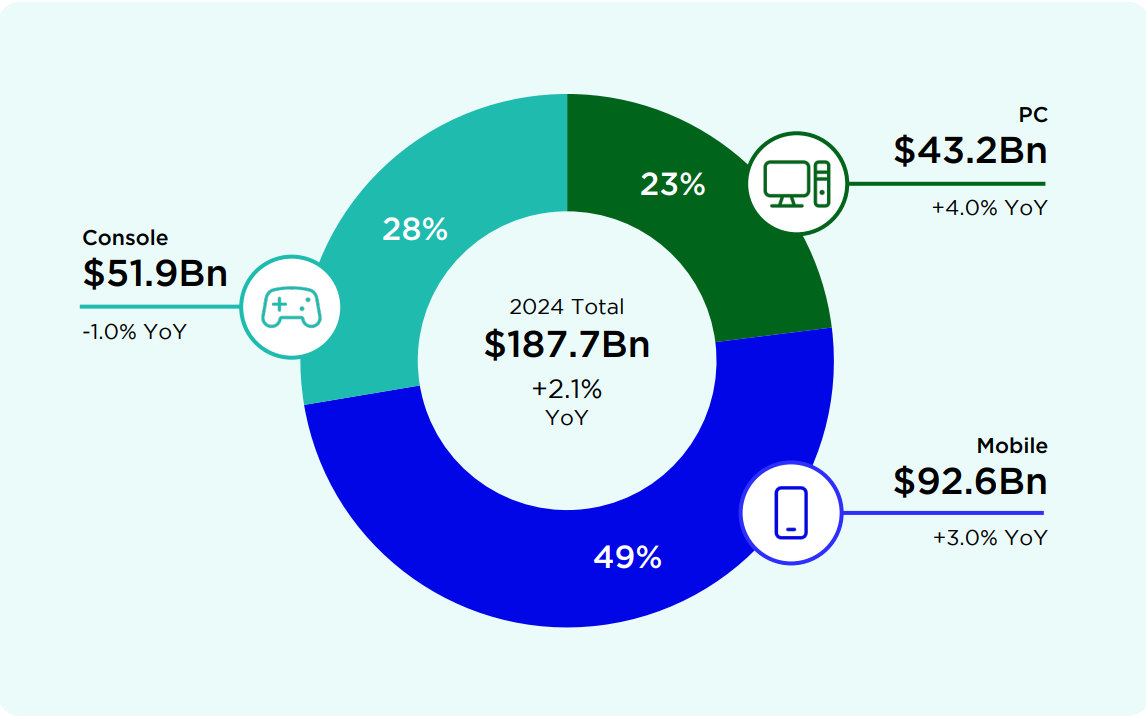
\includegraphics[width = 0.5\textwidth]{Imagenes/Newzoo_2024_Revenues.png}
	\caption{Ingreso estimado en la industria de videojuegos 2024.Newzoo}
	\label{fig:NewZooRevenues}
\end{figure}

\begin{figure}[H]
	\centering
	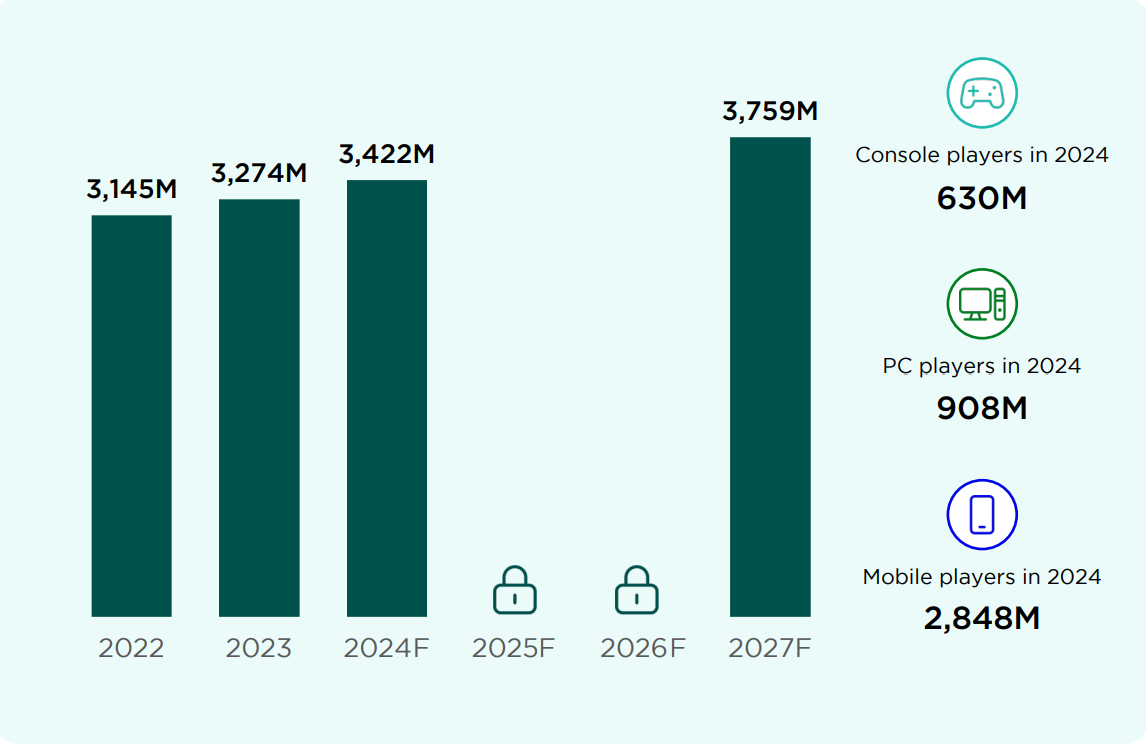
\includegraphics[width = 0.5\textwidth]{Imagenes/Newzoo_Players.png}
	\caption{Jugadores globales 2022-2024 y predicción en 2027.Newzoo}
	\label{fig:NewzooPlayers}
\end{figure}

Además en el mismo informe se comenta el porcentaje de jugadores de cada región ocupando más de la mitad, un 53\% los jugadores pacifico asiáticos como se muestra en la figura \ref{fig:NewzooPlayersReg}.
Con esos crecimientos y estos datos viene la necesidad de adaptar los videojuegos a diferentes lenguajes y culturas a través de los procesos de internacionalización ({\textit{I18N}}) y localización ({\textit{L10N}}) para poder ser publicados en otras regiones y países.
\begin{figure}[H]
	\centering
	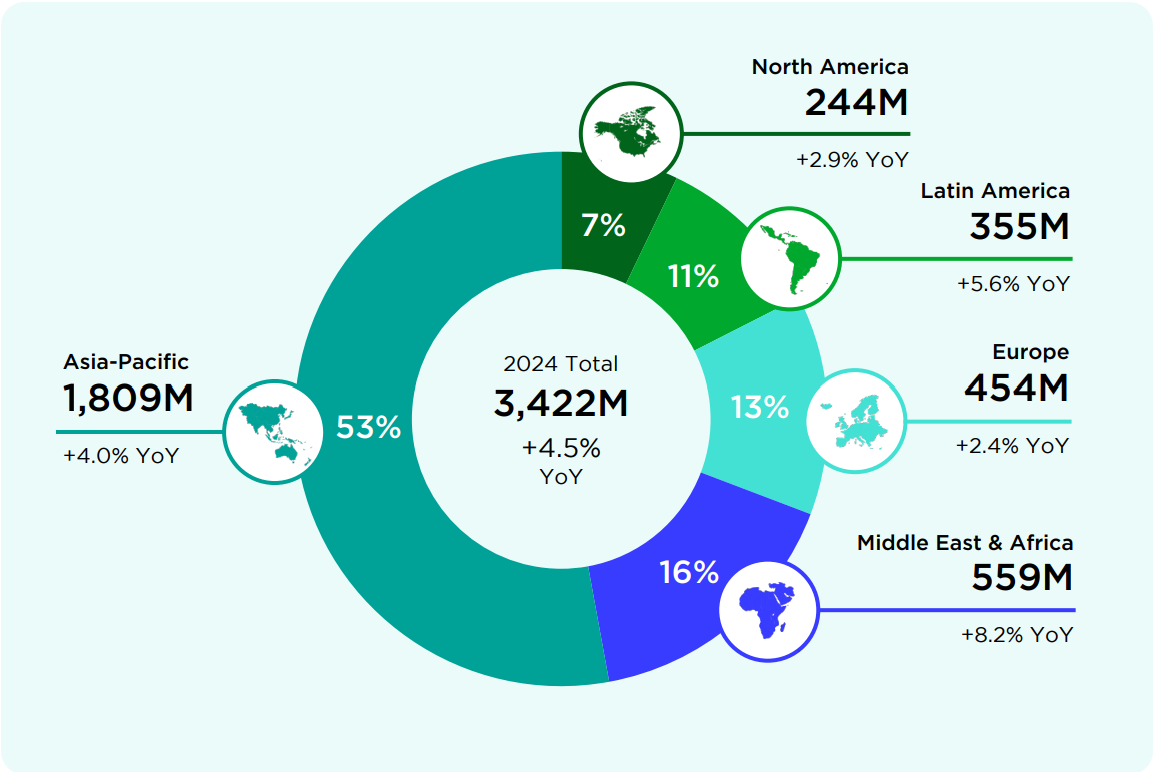
\includegraphics[width = 0.5\textwidth]{Imagenes/Newzoo_Players_Region.png}
	\caption{Porcentaje de jugadores de cada región. Newzoo}
	\label{fig:NewzooPlayersReg}
\end{figure}
La internacionalización es el proceso por el cual un videojuego se prepara desde sus etapas iniciales de desarrollo para soportar diferentes culturas e idiomas, de tal manera que no haya que realizar grandes modificaciones en el código para introducirlos.
Por otra parte, la localización es el proceso por el cual se traducen y adaptan los textos, gráficos y recursos de un videojuego para las diferentes culturas en las que éste se va a comercializar.

Durante ambos de estos procesos se pueden producir distintos tipos de errores (como errores de traducción o errores de visualización). Aquí es donde entra el \textit{Localization Quality Assurance} (o LQA). Este proceso se encarga de revisar y probar las distintas partes del videojuego para asegurarse de que no se produzca ninguno de estos errores y el producto final sea adecuado para las culturas y el público objetivo.

Hasta ahora este proceso ha sido un trabajo manual en el que los probadores comprueban meticulosamente cada texto y como éstos se visualizan dentro del videojuego, lo cual requiere de una gran cantidad de tiempo y recursos. Aunque existen herramientas para comprobar la corrección de las traducciones y los textos automáticamente, sin embargo, no se puede decir lo mismo en lo referente a comprobar que los textos se visualicen correctamente en el contexto del videojuego.

Teniendo en cuenta lo expuesto en los párrafos anteriores anterior, nuestra motivación para este trabajo es poder automatizar las pruebas sobre los procesos de internacionalización y localización, de forma que se puedan
ahorrar tiempo y recursos en estos campos y dedicarlos a otros más importantes. Para conseguir esto, vamos a utilizar técnicas de visión por computador y Reconocimiento óptico de caracteres \textit{(OCR,Optical Character Recognition)}
de forma que a partir de una captura de pantalla del videojuego, se pueda extraer el texto y realizar distintas comprobaciones y pruebas sobre él.


\section{Objetivos}
El objetivo principal en este trabajo es el diseño y la implementación de una herramienta que ayude en la automatización del QA en la localización.
Para lograr el objetivo principal, se plantea los siguientes objetivos secundarios: 
\begin{enumerate}

	\item Investigar sobre el proceso y las herramientas utilizadas en LQA, además de los errores más comunes en internacionalización y localización.
	\item Investigar sobre OCRs y cómo utilizarlas, para elegir una adecuada a nuestras especificaciones, realizando pruebas y comparaciones entre ellas.
	\item Diseñar una serie de tests automáticos basado en OCR para los posibles errores lingüísticos.
	\item Despliegue de la herramienta en una imagen de Docker para que pueda desplegarse en cualquier equipo.
	\item Integrar el OCR para usarlo como entrada de datos a los tests. Hacer mejoras para que el OCR de el máximo acierto posible.
	\item Evaluar nuestra herramienta para asegurar de que produce un porcentaje de acierto adecuado.
\end{enumerate}
\section{Plan de trabajo}
Para conseguir nuestros objetivos, seguiremos los siguientes pasos:
\begin{enumerate}
	\item Investigar y entender como funciona el proceso de internacionalización(\ref{sec:Internacionalización}), localización(\ref{sec:Localization}), el proceso de LQA(\ref{sec:LQA}) y los errores de lingüísticos más comunes(\ref{sec:Errores de localizacion}) que se producen a la hora de elaborar un videojuego. 
	\item Elegir de los errores más comunes de localización aquellas que estén relacionados con errores de caracteres o posiciones que sea posible ser detectado utilizando una OCR.(\ref{sec:Descripción de los tests})
	\item Elaborar una serie de tests que sean capaz de detectar si existe algún error de localización específico teniendo información de entrada de la OCR.(\ref{sec:Implementación de los tests})
	\item Investigar sobre distintos OCRs, ver como funcionan, como usarlos para detectar texto en imágenes, como entrenar un modelo sabiendo el idioma y la fuente usada.(\ref{sec:Seleccion de libreria de OCR})
	\item Hacer una evaluación con los OCRs seleccionados teniendo en cuenta el tiempo y el porcentaje de acierto.Buscar formas que aumente ese porcentaje de acierto.(\ref{sec:Mejoras en el reconocimiento})
	\item Hacer una evaluación por separado del funcionamiento de cada módulo (OCR, test).
	\item Unificar ambos módulos y hacer una evaluación completa de la herramienta.
	\item Generar una salida que sea fácilmente interpretado por un ser humano. 
	
\end{enumerate}
\section{Conclusion}
En conclusión, la industria de los videojuegos ha estado evolucionando de forma rápida, por lo que surge nuevas necesidades como llevar el videojuego de un idioma a otro adaptándose al país o la región. Para ello es necesario técnicas como la internacionalización y la localización en el videojuego. Para ahorrar trabajo humano, se propone un herramienta que pueda automatizar las pruebas sobre los procesos de internacionalización y localización.

\chapter{Estado de la Cuestión}
\label{cap:estadoDeLaCuestion}

%%En el estado de la cuestión es donde aparecen gran parte de las referencias bibliográficas del trabajo. Una de las formas más cómodas de gestionar la bibliografía en {\LaTeX} es utilizando \textbf{bibtex}. Las entradas bibliográficas deben estar en un fichero con extensión \textit{.bib} (con esta plantilla se proporciona el fichero biblio.bib, donde están las entradas referenciadas más abajo). Cada entrada bibliográfica tiene una clave que permite referenciarla desde cualquier parte del texto con los siguiente comandos:%

%\begin{itemize}
%\item Referencia bibliografica con cite: \cite{ldesc2e}
%\item Referencia bibliográfica con citep: \citep{notsoshort}
%\item Referencia bibliográfica con citet: \citet{latexAPrimer}
%\end{itemize}

%Es posible citar más de una fuente, como por ejemplo \citep{latexCompanion,LaTeXLamport,texKnuth}

%Después, \LaTeX se ocupa de rellenar la sección de bibliografía con las entradas \textbf{que hayan sido citadas} (es decir, no con todas las entradas que hay en el .bib, sino sólo con aquellas que se hayan citado en alguna parte del texto).

%Bibtex es un programa separado de latex, pdflatex o cualquier otra cosa que se use para compilar los .tex, de manera que para que se rellene correctamente la sección de bibliografía es necesario compilar primero el trabajo (a veces es necesario compilarlo dos veces), compilar después con bibtex, y volver a compilar otra vez el trabajo (de nuevo, puede ser necesario compilarlo dos veces). 

\section{Internacionalización}
La internacionalización es el proceso de preparar un producto para que pueda admitir diferentes idiomas y convenciones culturales sin necesidad de volver a rediseñarse.(Localisation Industry Standards Association)(LISA).

Separación del texto traducible de código fuente: Esto ayuda a que el traductor se centre únicamente en el trabajo de traducción y no tenga que acceder al código fuente.

Uso de fuentes adecuadas para distintos idiomas: Las fuentes deben mostrar todos los posibles caracteres del idioma seleccionado, el fallo de esto puede conllevar a que en el videojuego no se vea el texto completo.

Uso de la codificación adecuada para distintos idiomas: Es necesario que la codificación pueda interpretar un carácter o símbolo introducido por teclado. Se usa el estándar de Unicode.

Diseño de interfaces adaptables al texto que se debe mostrar: La misma cadena de texto en distintos idiomas traducidos pueden necesitar distintos espacios para mostrarlo en pantalla, esto puede conllevar a un problema a la hora de diseñar la interfaz y el espacio que tiene en el videojuego para mostrar una cadena.
Se plantean las siguientes posibilidades de solucionar el problema

\begin{itemize}
\item Uso de fuente de ancho variable siempre que sea posible: La fuente elegida afecta mucho a la hora de mostrar más o menos caracteres. Existen las fuentes de ancho fija (todos los caracteres ocupan exactamente el mismo número de píxeles), fuentes de ancho variable (cada carácter ocupa un determinado número de píxeles). Poner ejemplos.
\item Uso de bocadillos, cajas o ventanas de texto adaptables al contenido: El tamaño de las ventanas se adaptará al tamaño de texto que hay dentro.
\item Uso de menús y botones con gran espacio o adaptables al contenido: En muchas ocasiones surge el problema de que el texto traducido no quepa en el espacio del botón o del menú, para ello se recomienda que se hagan con espacio suficiente para abordar cualquier posible tamaño de la traducción o que sean adaptables al contenido.
\end{itemize}

Uso de etiquetas especiales para marcar género, sexo o número: Un problema a la hora de traducir reside en la concordancia de género, sexo y número en distintos idiomas, un ejemplo es \textit{``You are so nice''} se puede traducir como ``Eres muy simpático'' o ``Eres muy simpática''. Por lo tanto es necesario la existencia de un sistema que cambie la palabra según si se trata de un personaje masculino o femenino.

Facilitación de un mínimo de información contextual: En distintos idiomas puede resultar que la traducción sea diferente dependiendo del contexto, esto el traductor no lo sabe, por lo tanto es necesario un mínimo de información contextual para agilizar el proceso de traducción.

Comprobación cultural de imágenes e iconos: Algunos gestos, imágenes o iconos pueden resultar inapropiados para algunas culturas o religiones hay que tener especial cuidado con la zona de localización.

\section{Localización}
\section{Language Quality Assurance LQA }
\section{Bugs Linguísticos comunes} \label{bugs}
A continuación haremos una enumeración de los distintos \textit{bugs} de localización que se pueden encontrar en un videojuego. \footnote{Las definiciones y nombres de estos bugs son sacados de \citet{LQAPSM2017}, a partir de la pág. 154}
\subsection{Problema de fuente} \label{ErrorFuente}
Este problema se da cuando la fuente utilizada no incluye alguno de los caracteres especiales de un idioma. Normalmente estos caracteres que faltan en la fuente se muestran como se puede ver en la Figura \ref{Notdef}

\begin{figure}[H]

	\centering
	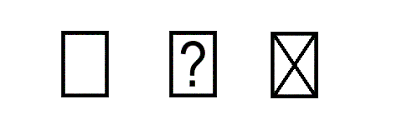
\includegraphics{Imagenes/BugsLQA/Notdef.png}
	\caption{Glifos con los que se representan habitualmente los caracteres no incluidos en una fuente}
	\label{Notdef}
\end{figure}
	
\subsection{Implementación de texto incorrecta}\label{ErrorImpIncorrecta}
Este error se produce cuando un texto que debería aparecer en un idioma se muestra en uno distinto, por ejemplo, alemán. Este error se puede producir porque hay texto equivocado documento de localización, o porque el programa tiene algún \textit{bug}. Debido a esto, el \textit{tester} tiene que verificar que la celda del documento tiene el texto adecuado.  
\subsection{Cadena no localizada}\label{ErrorNoLocalizada}
Este error se produce cuando un texto no está traducido. Puede deberse tanto a que el traductor no haya traducido el texto, como a que el desarrollador no haya facilitado dicho texto para la traducción. 
\subsection{Error tipográfico o de ortografía}\label{ErrorTypo}
Este error se produce cuando el texto tiene algún tipo de error ortográfico o errata.

\subsection{Error gramatical}\label{ErrorGramatical}
Este error se produce cuando el texto tiene un fallo gramatical.

\subsection{Error de traducción}\label{ErrorTraducción}
Este error se da cuando la traducción de un texto es errónea, ya sea por una traducción incorrecta (p. ej. ``Monedas de cobre'' a ``gold''); por falta de información u omisión de palabras; o porque el texto no tenga sentido en el contexto (p. ej al traducir desde el japonés).

\subsection{Solapamiento de texto}\label{ErrorSolapamiento}
Este error se produce cuando el texto sobresale de los límites de un botón o cuadro de diálogo. Puede deberse a una mala implementación por parte del desarrollador, o a que el traductor no ha respetado los límites de espacio que se le han dado.

\subsection{Truncamiento de texto}\label{ErrorTruncamiento}
Este error es el caso contrario al anterior. En este caso, el texto en lugar de salirse de los límites, queda cortado por ellos y no se muestra al completo.

\subsection{Error terminológico o incoherencia}\label{ErrorTermino}
Este error se produce cuando se usa una palabra incorrecta para referirse a una terminología clave (p. ej. utilizar el término ``grabar'' en lugar de ``guardar''). También puede darse cuando el mismo término no está escrito de la misma manera en dos lugares distintos (p. ej. Escribir un término importante en minúsculas en un lugar y en mayúsculas en otro.).

\subsection{Incumplimiento de directrices}\label{ErrorDirectrices}
Este error se da cuando una traducción no se cumplen las reglas de estilo que impone un distribuidor o plataforma para los videojuegos que se publiquen en ella. Por ejemplo, los mensajes del sistema en videojuegos en consolas deben de escribirse exactamente como aparecen en unas listas oficiales preparadas por las compañías que venden estas consolas.

\subsection{Error de subtítulos}\label{ErrorSubtitulos}
Este error tiene varias formas. Las más habituales son:
\begin{itemize}
	\item Los subtítulos no aparecen.
	\item Los subtítulos están desicronizados con el audio.
	\item No da tiempo a leer los subtítulos.
	\item Los subtítulos no están bien segmentados.
	\item Los subtítulos no coinciden con el contenido doblado. 
\end{itemize}

\subsection{Error de audio}\label{ErrorAudio}
Al igual que con los subtítulos, este error tiene varias formas:
\begin{itemize}
	\item El diálogo no se escucha o está en el idioma original
	\item El audio no está bien sincronizado con los gráficos.
	\item El audio no coincide con el contexto.
\end{itemize}

\subsection{Problemas culturales}\label{ErrorCultura}
Este error se suele dar cuando en un videojuego se utiliza alguna simbología o gesto que tiene un significado ofensivo en otra cultura. Un ejemplo puede ser la utilización del símbolo \textit{manji} en un juego japonés, que es muy parecido a la esvástica de la Alemania nazi.
\begin{figure}[h]
	
	\centering
	
\includegraphics{Imagenes/BugsLQA/Manji.jpg}
	\caption{Comparación entre el \textit{manji} y la esvástica.}
	\label{Manji}
\end{figure}

%\begin{itemize}
%	\item Problema de fuente: La fuente utilizada no incluye alguno de los caracteres especiales de un idioma, por ejemplo las tildes (á), la ñ en español.
%	\item Implementación de texto incorrecta: Sucede cuando el texto debería aparecer en un idioma, aparece en un idioma diferente. Puede suceder por un descuido del desarrollador.
%	\item Cadena no localizada: Tiene lugar cuando la cadena de texto no viene traducida en el juego, puede deberse a un fallo del desarrollador.
	%\item Error tipográfico
	%\item Error gramatical
%	\item Error de traducción: Cuando el texto traducido no tiene el mismo significado que el texto original, o que no tiene sentido en ese contexto
	%\item Solapamiento de texto: Cuando el texto escrito es más largo de lo esperado por el programador por lo que se sale de los límites del espacio guardado para ese texto y se solapan. 
	%\item Texto truncado: Contrario al solapamiento de texto, el texto no se muestra de forma completa.
%	\item Error terminológico
%	\item Incoherencia
%	\item Incumplimiento de instrucciones: Tiene que ver con no seguir unas instrucciones del proyecto, por ejemplo en el mundo de las consolas, un tipo de error tiene que escribirse de una forma en concreta, saltarse esa norma supone retrasos en la aprobación del producto.
%	\item Error de estilo
%	\item Error subtítulos
%	\item Error de audio
%	\item Problemas culturales
%\end{itemize}

\section{Reconocimiento Óptico de Caracteres (OCR)}
El OCR (Reconocimiento Óptico de Caracteres, por sus siglas en inglés Optical Character Recognition) es una tecnología que convierte imágenes de texto manuscrito, impreso o mecanografiado en datos de texto que las computadoras pueden interpretar y manipular. En otras palabras, puede extraer el texto contenida en una imagen.

Para llegar al objetivo de reconocer el texto y extraerlo de la imagen el OCR da una serie de pasos	\footnote{(Extracting text from an image using Ocropus) \url{https://www.danvk.org/2015/01/09/extracting-text-from-an-image-using-ocropus.html} }	\footnote{(Improving the quality of the output) \url{https://tesseract-ocr.github.io/tessdoc/ImproveQuality.html} }:
\begin{enumerate}
	\item \textbf{Preprocesamiento de la imagen:}
	
	El propósito de este paso es procesar la imagen para que sea más legible para la computadora y reconocer así de forma mas eficiente los textos.
	\begin{itemize}
		\item Conversión a escala de grises: La mayoría de los OCR primero convierten la imagen en blanco y negro o escala de grises para simplificar el procesamiento.
		\item Reducción de ruido: Se aplican filtros para eliminar manchas, borrones o marcas en la imagen que puedan afectar la precisión del reconocimiento.
		\item Binarización: La imagen se convierte a una representación en blanco y negro, donde los píxeles se clasifican como parte del fondo (blanco) o del texto (negro). Este proceso ayuda a aislar los caracteres.
	\end{itemize}
	
	\item \textbf{Segmentación:}
	
	El OCR divide la imagen en secciones manejables. Primero separa líneas de texto.  Luego separa las palabras y finalmente descompone las palabras en caracteres individuales. Este paso es crucial, ya que el OCR necesita reconocer los caracteres de manera individual, pero considerando también su contexto dentro de una palabra o frase.
	
	\item \textbf{Detección de características:}
	
	Extracción de características de los caracteres: El OCR analiza los caracteres y sus formas, midiendo varios atributos como las líneas, contornos, cruces de líneas, y la disposición de los píxeles. Estos datos son usados para diferenciar letras, números y símbolos similares (como ``O'' y ``0'' o ``l'' y ``1'').
	Se aplican técnicas basadas en modelos geométricos, estructuras de redes neuronales o de aprendizaje automático para identificar patrones comunes en los caracteres.
	
	\item \textbf{Reconocimiento del carácter:}
	
	Clasificación de los caracteres: Una vez identificadas las características, el OCR las compara con una base de datos o ``alfabeto'' interno de posibles caracteres. Esto puede hacerse de varias maneras, dependiendo del tipo de OCR\footnote{(¿Qué es el reconocimiento óptico de caracteres (OCR)?) \url{https://aws.amazon.com/es/what-is/ocr/} }:
	\begin{itemize}
		\item Métodos basados en plantillas: Se compara cada carácter con un conjunto de plantillas predefinidas. Si la forma del carácter coincide con una plantilla, se clasifica como ese carácter.
		\item Métodos basados en aprendizaje automático o redes neuronales: Las técnicas modernas de OCR suelen usar redes neuronales entrenadas con miles de ejemplos de texto. El sistema ``aprende'' a identificar caracteres y a hacer distinciones más sutiles en base a sus experiencias pasadas.
	\end{itemize}

	
	
\end{enumerate}

\chapter{Descripción del Trabajo}
\label{cap:descripcionTrabajo}

Aquí comienza la descripción del trabajo realizado. Se deben incluir tantos capítulos como sea necesario para describir de la manera más completa posible el trabajo que se ha llevado a cabo. Como muestra la figura \ref{fig:sampleImage}, está todo por hacer.

\begin{figure}[H]
	\centering
	
\includegraphics[width = 0.5\textwidth]{Imagenes/Vectorial/Todo.pdf}
	\caption{Ejemplo de imagen}
	\label{fig:sampleImage}
\end{figure}

Si te sirve de utilidad, puedes incluir tablas para mostrar resultados, tal como se ve en la tabla \ref{tab:sampleTable}.


\begin{table}
	\centering
	\begin{tabular}{c|c|c}
		\textbf{Col 1} & \textbf{Col 2} & \textbf{Col 3} \\
		\hline\hline
		3 & 3.01 & 3.50\\
		6 & 2.12 & 4.40\\
		1 & 3.79 & 5.00\\
		2 & 4.88 & 5.30\\
		4 & 3.50 & 2.90\\
		5 & 7.40 & 4.70\\
		\hline
	\end{tabular}
	\caption{Tabla de ejemplo}
	\label{tab:sampleTable}
\end{table}
	
\section{Selección de librerías de OCR (Optical Character Recognition)}
Durante el desarrollo de este trabajo, se evaluaron varias herramientas de OCR para seleccionar la más adecuada para nuestras necesidades. Las herramientas probadas fueron OCRopus, EasyOCR y Tesseract. A continuación, se describe brevemente cada una de ellas.
\begin{enumerate}
	\item \textbf{OCRopus}
	\footnote{(repositorio github de OCRopus) \url{https://github.com/ocropus-archive/DUP-ocropy} }
	Es un sistema de OCR basado en redes neuronales con un enfoque modular.
	Principalmente esta disponible para Linux. Proporciona diferentes módulos para la binarización , segmentación ,generación del ground-truth y el entreno del modelo.
	Se ha utilizado la herramienta para reconocer la imagen de prueba pero el resultado fue que no consiguió reconocer ningún texto , por lo que fue descartado ya que las otras alternativas que hablaremos en adelante si que ha conseguido algo.
	Otras razones por la que esta herramienta fue descartado es que el lenguaje de programación principal con la que trabaja es \emph{python} y en nuestro proyecto trabajamos principalmente con \emph{c++}. Además la última actualización de esta librería fue en 16 de Diciembre de 2017
	
	\item \textbf{EasyOCR}
	EasyOCR es una biblioteca de reconocimiento óptico de caracteres (OCR) desarrollada en Python que facilita la extracción de texto de imágenes y documentos. Diseñada con el objetivo de ser fácil de usar y accesible, una de las características de EasyOCR es que es capaz de reconocer texto en más de 80 idiomas y soporta múltiples scripts, lo que la convierte en una herramienta versátil para diversas aplicaciones.
	La herramienta es fácil de usar y ofrece buenos resultados al reconocimiento.
	Proporciona gran variedad de modelos entrenados y también ofrece la opción de entrenar tu propio modelo.
	
	La herramienta en resumen se adapta muy bien a nuestras necesidades. El único problema esta en el idioma de programación con la que trabaja , al igual que OCRopus , EasyOCR está implementada con \emph{python} y nosotros con \emph{c++} , esto no supone un gran problema pero hemos encontrado una mejor solución.
	
	\item \textbf{Tesseract}
	
	Tesseract es una biblioteca de (OCR) de código abierto que se utiliza para convertir imágenes de texto en texto editable. Originalmente desarrollado por Hewlett-Packard en la década de 1980, Tesseract fue liberado como software de código abierto en 2005 y ha sido mantenido y mejorado por la comunidad, particularmente por Google, que ha contribuido significativamente a su desarrollo.
	
	Al igual que EasyOCR una de las características más destacadas de Tesseract es su capacidad para reconocer texto en múltiples idiomas y alfabetos, soportando más de 100 idiomas de forma nativa. Esto lo convierte en una herramienta versátil para aplicaciones globales que requieren la extracción de texto de documentos escritos en diferentes lenguas.
	
	Tesseract utiliza técnicas avanzadas de aprendizaje profundo y redes neuronales, lo que le permite alcanzar altos niveles de precisión en el reconocimiento de texto. Su arquitectura se basa en el uso de modelos de aprendizaje profundo entrenados con grandes conjuntos de datos, lo que mejora continuamente su rendimiento en diversas condiciones.
	
	El motor puede integrarse fácilmente en aplicaciones de procesamiento de imágenes y visión por computadora. Tesseract se utiliza comúnmente en combinación con bibliotecas como OpenCV para preprocesar imágenes antes de la etapa de reconocimiento, lo que mejora la precisión de los resultados.
	
	Además, Tesseract ofrece una API en varios lenguajes de programación, lo que facilita su integración en diferentes entornos de desarrollo y una de ellas es C++, por lo que esta herramienta cumple con todos los requisitos para nuestro proyecto y es la razón por la que hemos optado por Tesseract.
\end{enumerate}
\subsection{Pruebas y resultados de los OCR}
Para evaluar los resultados de los OCRs y hacer la elección del OCR a utilizar se tiene en cuenta el tiempo de ejecución necesario para reconocer los caractéres y el CER(Character Error Rate).


\textbf{CER (Character Error Rate)} \footnote{(Char Error Rate — PyTorch-Metrics 1.5.2 documentation)\url{https://lightning.ai/docs/torchmetrics/stable/text/char_error_rate.html} }
El CER es una métrica usada comúnmente para evaluar la precisión de un sistema de reconocimiento de caracteres (OCR) u otros sistemas que transcriba texto.El valor se obtiene calculando el número de errores a nivel de carácter dividido por el número total de caracteres en el texto de referencia.
Los errores pueden ser de:
\begin{enumerate}
	\item Sustituciones: Un carácter incorrecto reemplaza a uno correcto.
	\item Inserciones: Aparece un carácter extra que no debería estar.
	\item Eliminaciones: Falta un carácter que debería estar presente.
\end{enumerate}
La fórmula general para calcular el CER es:
	
	$CER = \frac{S+D+I}{N} $ 



Donde:

S es el número de sustituciones.

D es el número de eliminaciones.

I es el número de inserciones.

N es el número total de caracteres en el texto de referencia.





El CER se expresa como un valor entre 0 y 1 (o como porcentaje), donde 0 significa que no hubo errores (transcripción perfecta) , 1 (o 100) indica que todos los caracteres son incorrectos.


La prueba se ha hecho con 13 imágenes elegidas de forma que se considera más fácil de reconocer(a ojo humano)las imágenes con menor número de identificación.
Las imágenes se pueden encontrar en el repositorio del trabajo en OCRTests/images.
Se utiliza la libreria Jiwer\footnote{(Jiwer Usage)\url {https://jitsi.github.io/jiwer/usage/}} en python para los cálculos de CER, para más detalles se puede mirar el archivo Jiwer\_Cer.py situado en OCRTests.

En los resultados de los ocr se encontrará un valor llamado CER medio ,este valor se obtiene calculando el número total de errores a nivel de carácter encontrado en toda la batería de prueba divido entre el número total de caracteres de toda la batería de prueba.
\begin{enumerate}
	\item \textbf{Tesseract}
	
	
	Resultados del CER de cada imágen y el CER medio
	\begin{verbatim}
		{
			"1": 0.0,
			"2": 0.0625,
			"3": 0.5384615384615384,
			"4": 0.043478260869565216,
			"5": 0.2890625,
			"6": 0.025,
			"7": 0.75,
			"8": 0.9347826086956522,
			"9": 0.7209302325581395,
			"10": 1.0,
			"11": 0.05,
			"12": 0.35172413793103446,
			"13": 0.22988505747126436,
			"CER medio": 0.3842941796913226
		}
	\end{verbatim}
	El tiempo transcurrido para finalizar el OCR ha sido de 5539 milisegundos.
	\begin{figure}[H]
		\centering
		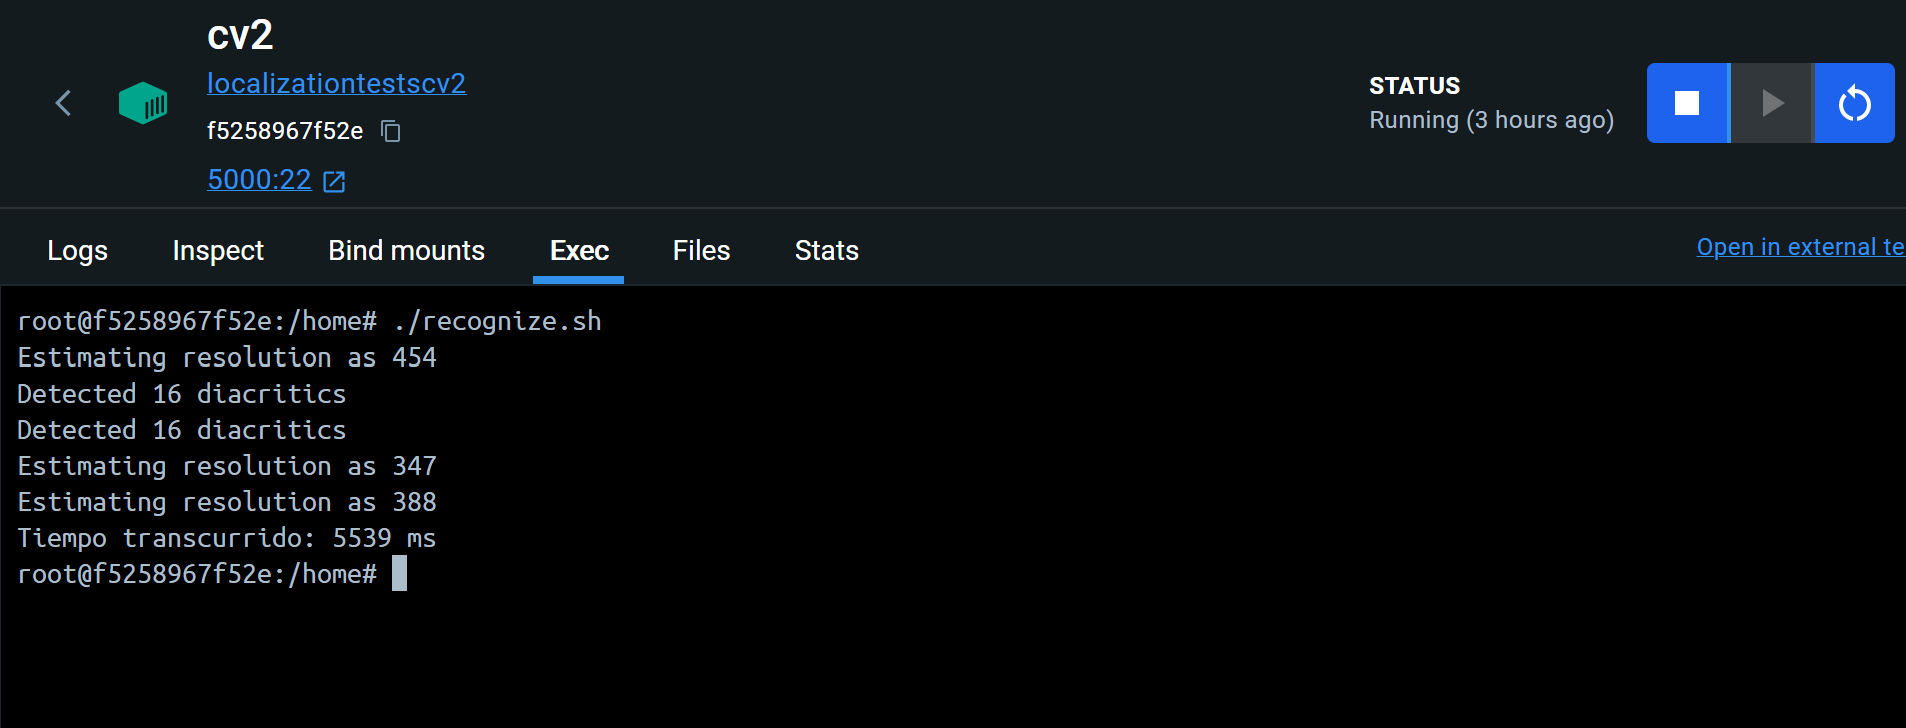
\includegraphics[width = 0.5\textwidth]{Imagenes/OCR/Tiempo_Tesseract.png}
		\caption{Tiempo transcurrido en la prueba usando Tesseract}
	\end{figure}
	\item \textbf{EasyOcr}
	
	Resultados del CER de cada imágen y el CER medio
	\begin{verbatim}
	
		{
			"1": 0.0,
			"10": 0.8571428571428571,
			"11": 0.15,
			"12": 0.05517241379310345,
			"13": 0.3371647509578544,
			"2": 0.28125,
			"3": 0.21153846153846154,
			"4": 0.10869565217391304,
			"5": 0.0859375,
			"6": 0.025,
			"7": 0.0,
			"8": 0.6521739130434783,
			"9": 0.2558139534883721,
			"CER medio": 0.23229919247215694
		}
	\end{verbatim}
	
		El tiempo transcurrido para finalizar el OCR ha sido de 204625 milisegundos.
	\begin{figure}[H]
		\centering
		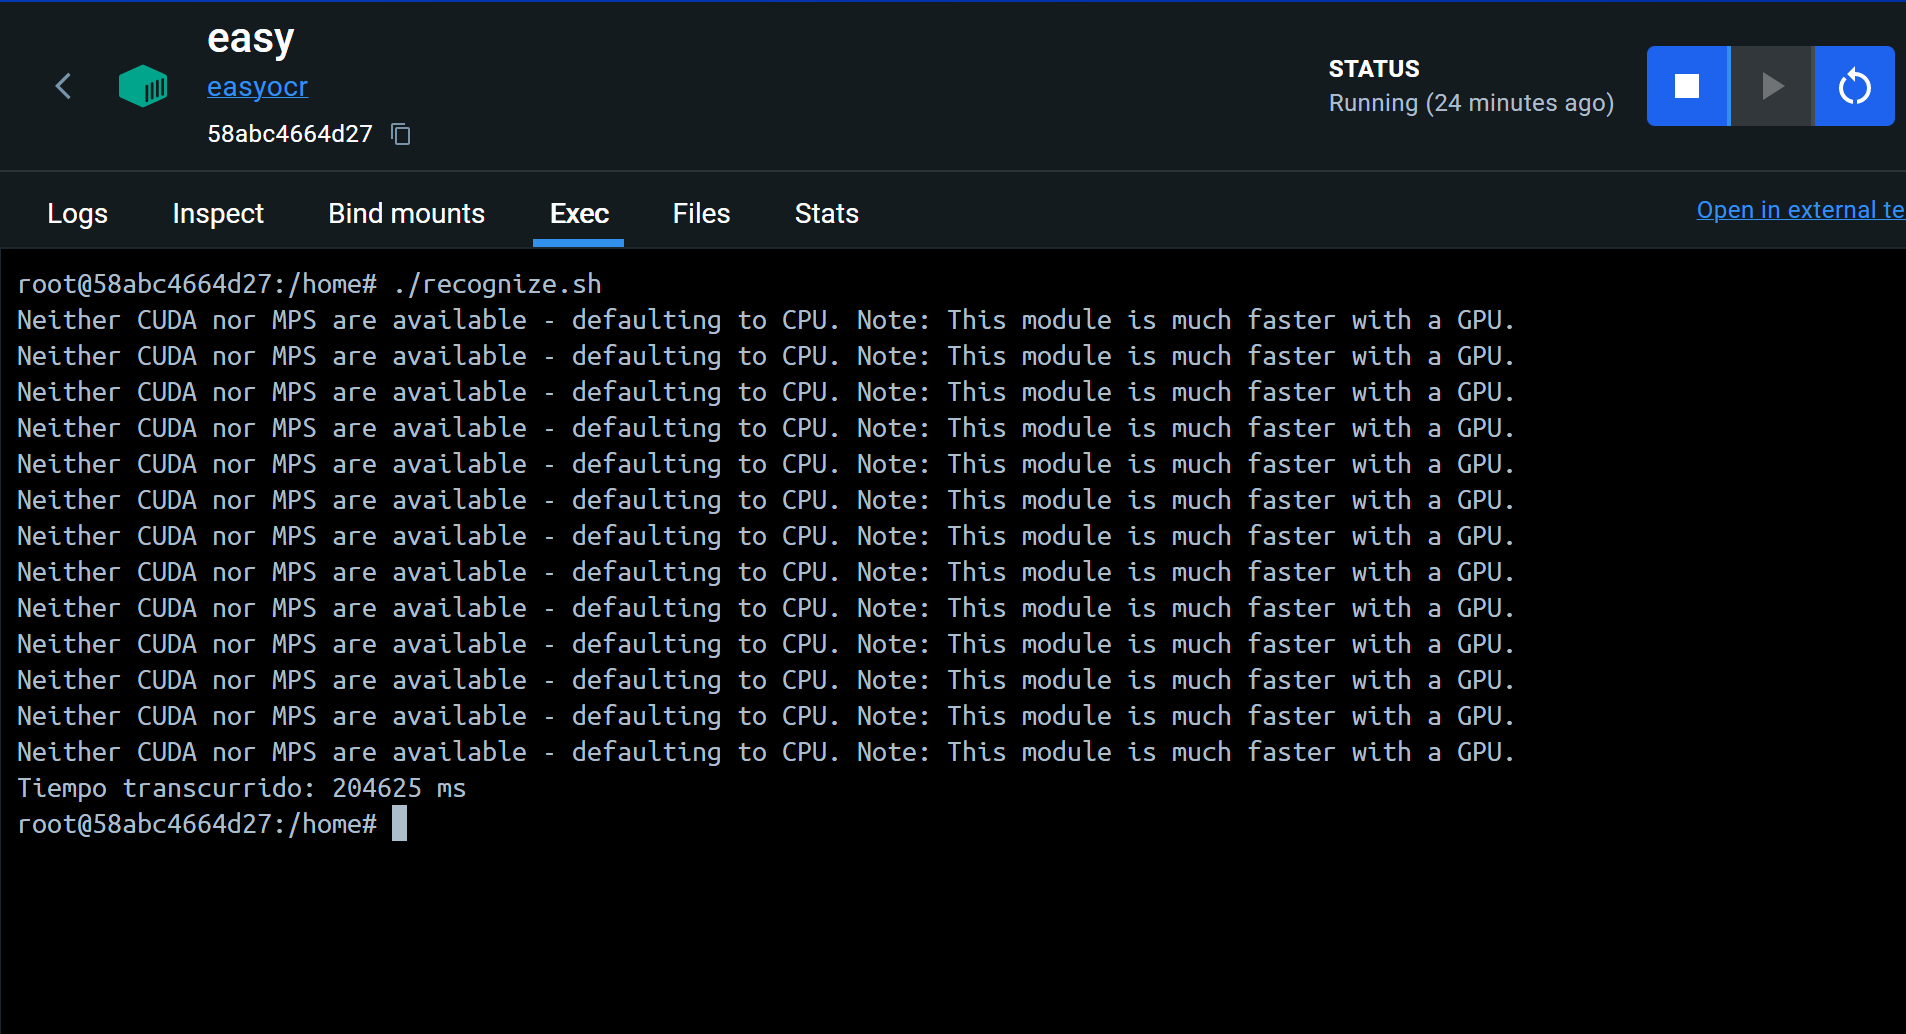
\includegraphics[width = 0.5\textwidth]{Imagenes/OCR/Tiempo_EasyOcr.png}
		\caption{Tiempo transcurrido en la prueba usando EasyOCR}
	\end{figure}
	
	\item \textbf{OCRopus}
	
		\begin{verbatim}
		
		{

		}
	\end{verbatim}
\end{enumerate}


Como se puede ver en los resultados obtenidos de los test realizados, tanto Tesseract y EasyOCR obtiene buenos resultados. Aunque EasyOCR obtiene un mejor CER medio en los resultados (0.23) que Tesseract (0.38), Tesseract es muchísimo más rápido que EasyOCR teniendo un 199086 milisegundo de adelanto que equivale a 3 minutos y medio. Por tanto decidimos seguir en adelante con Tesseract.



\section{Mejoras en el reconocimiento de texto en imágenes}
En este trabajo es muy importante que la entrada de los test sea correctos ya que todos nuestros test se basan en ello, por lo que se propone mejoras para aumentar la precisión del texto obtenido por el OCR disminuyendo el CER.

\textbf{Clasificación de imágenes de pruebas}

Para obtener más información sobre aquellos factores o características de las imágenes que puedan afectar al rendimiento y efectividad de la herramienta de OCR, se ha clasificado las imágenes en 5 categorías diferentes,la clasificación se ha hecho a ojo humano de forma subjetiva.
\begin{enumerate}
	\item Fondos simples.
		\begin{figure}[H]
		\centering
		
\includegraphics[width = 0.5\textwidth]{Imagenes/OCR/Simple.png}
		\caption{Ejemplo imagen fondos simples }
	\end{figure}
	
	\item Fondos complejos.
		\begin{figure}[H]
		\centering
		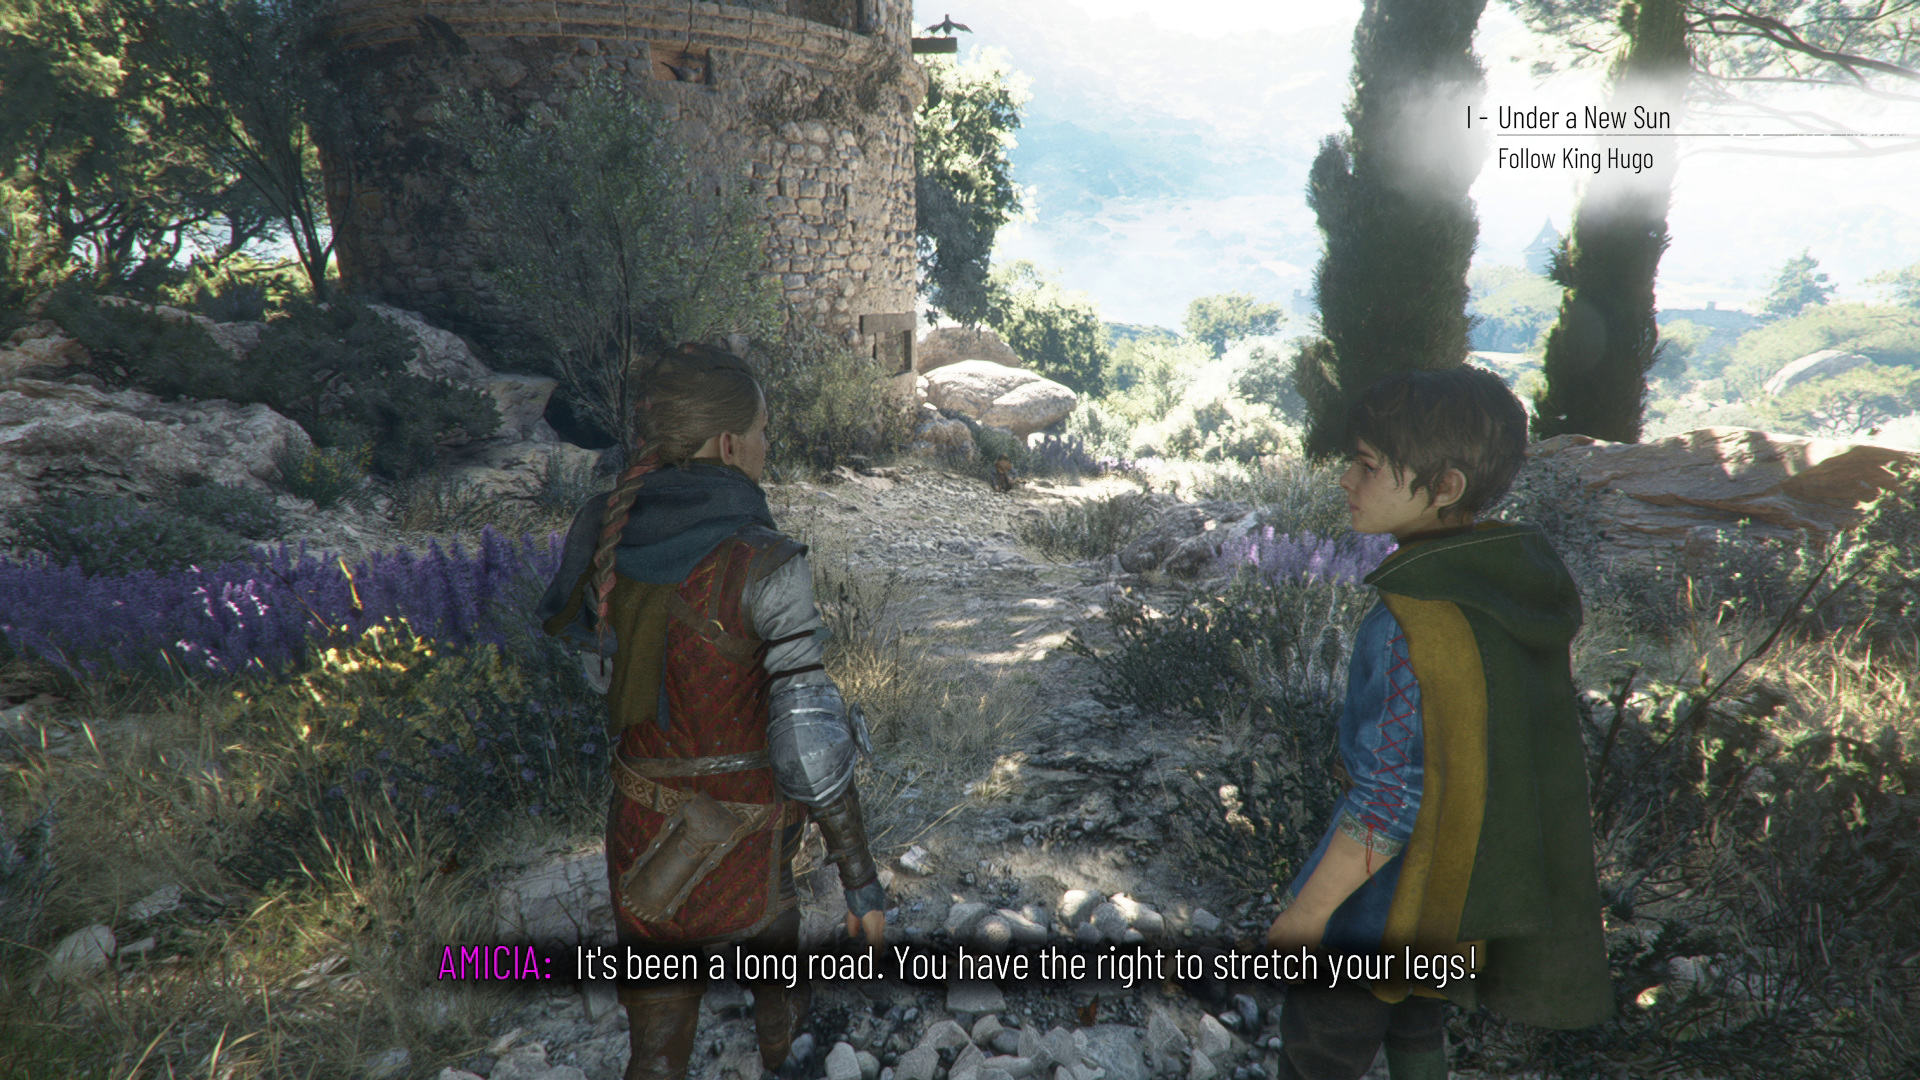
\includegraphics[width = 0.5\textwidth]{Imagenes/OCR/Complejo.png}
		\caption{Ejemplo imagen fondos complejos }
	\end{figure}
	\item PixelArt.
		\begin{figure}[H]
		\centering
		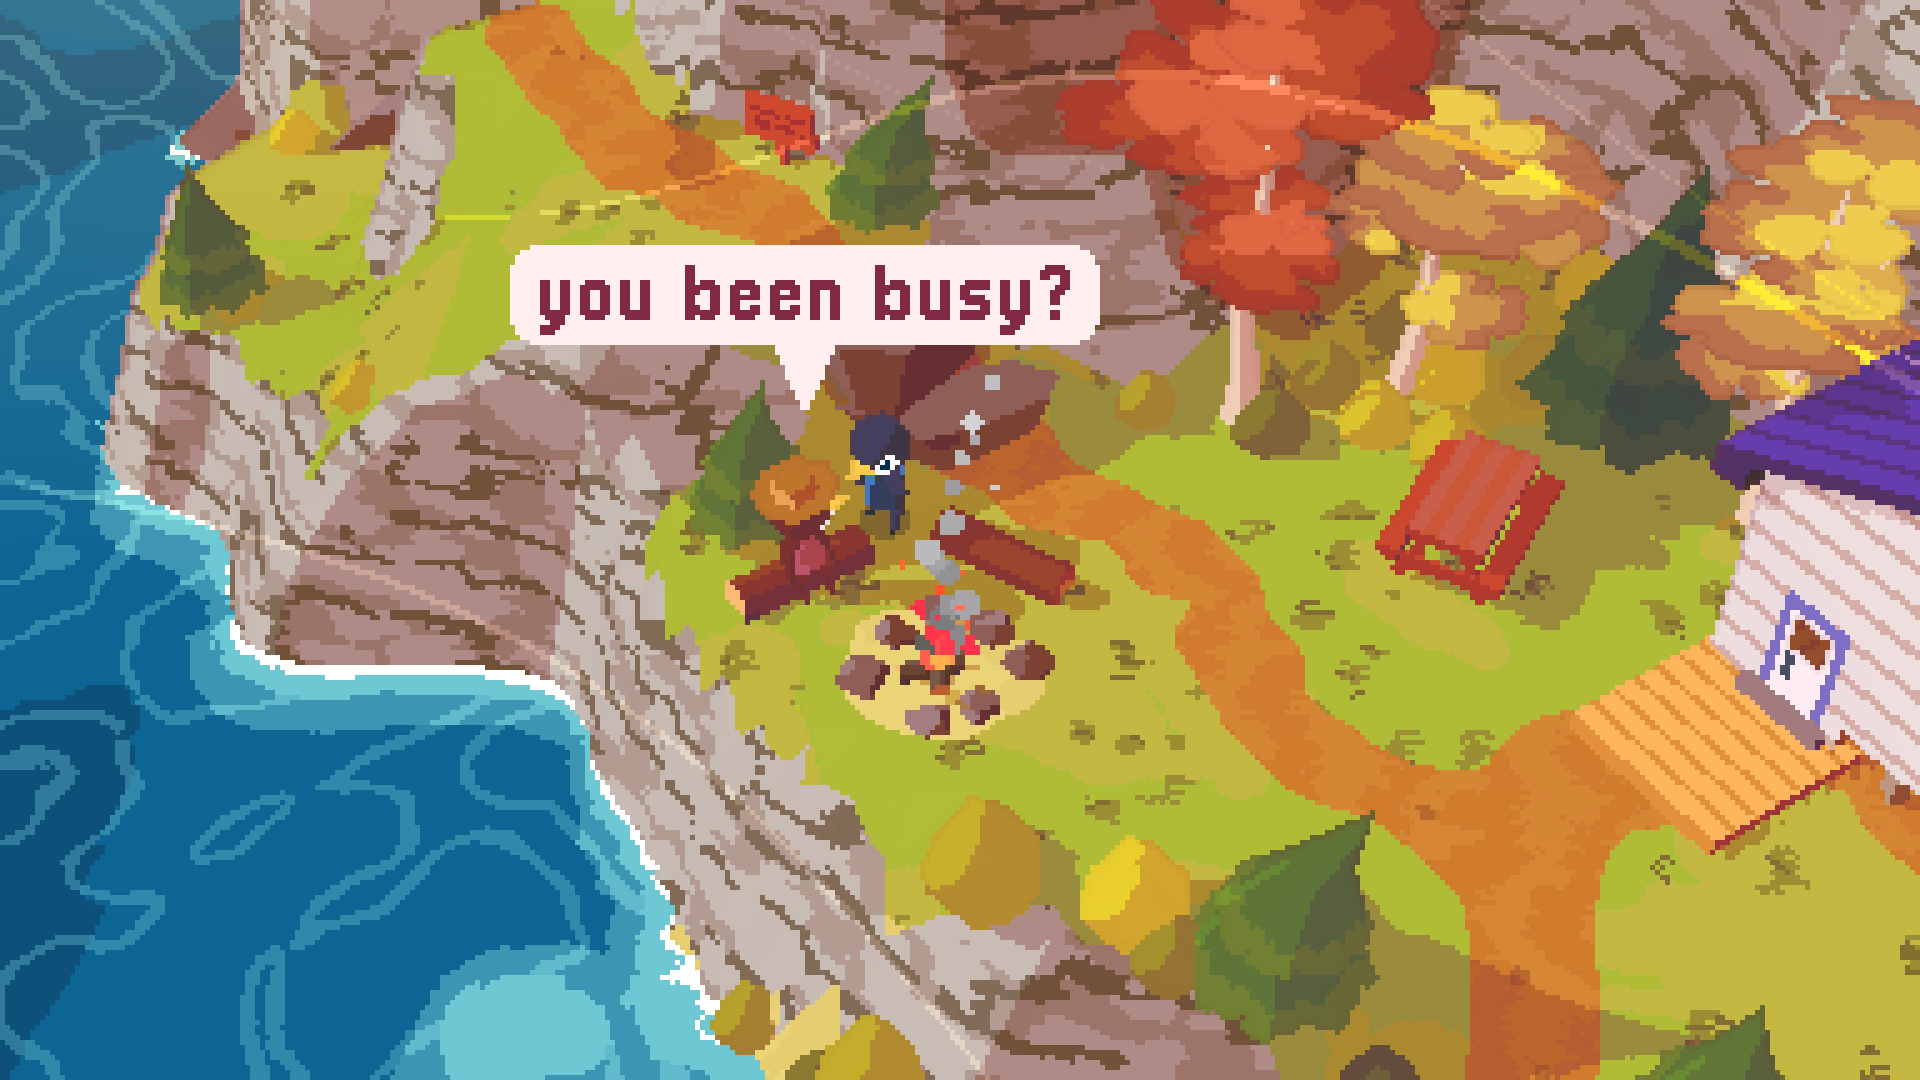
\includegraphics[width = 0.5\textwidth]{Imagenes/OCR/Pixel.png}
		\caption{Ejemplo imagen PixelArt }
	\end{figure}
	\item Texto en bocadillos.
		\begin{figure}[H]
		\centering
		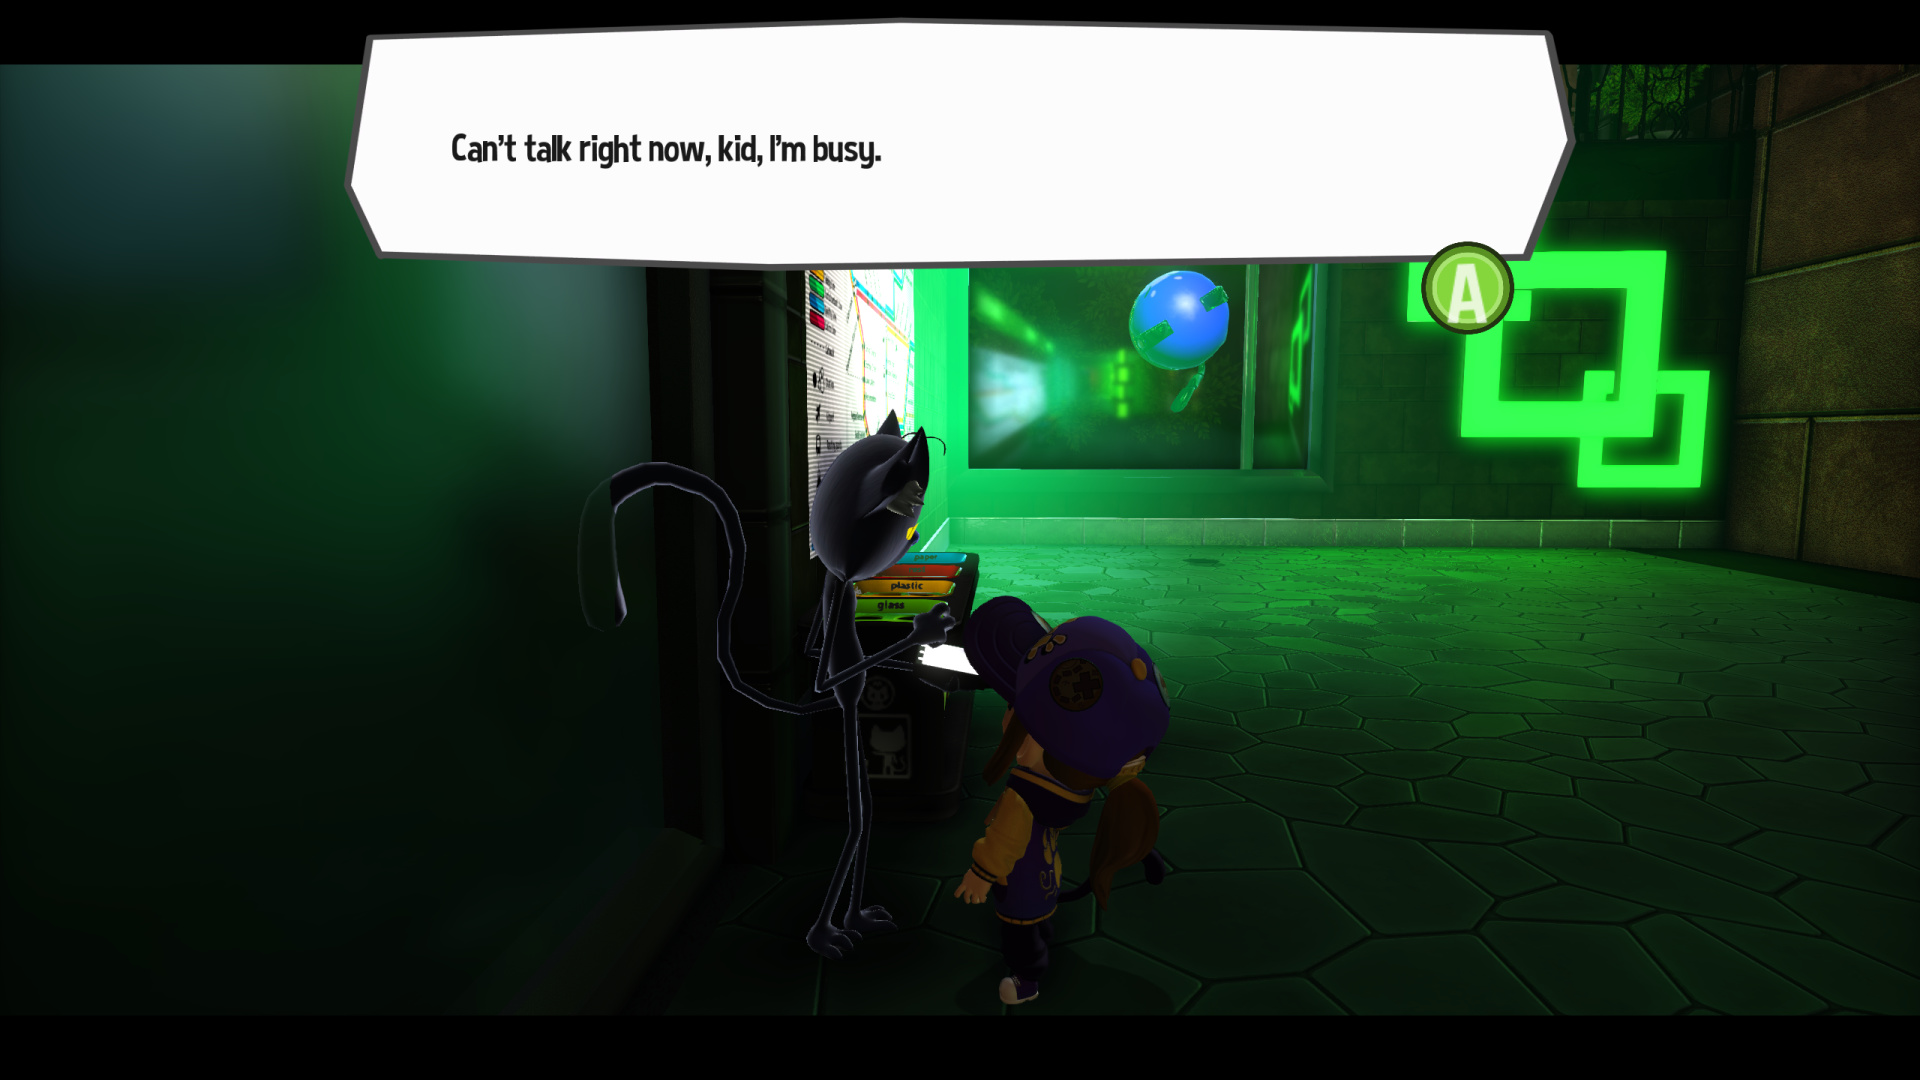
\includegraphics[width = 0.5\textwidth]{Imagenes/OCR/Boc.png}
		\caption{Ejemplo imagen de texto en bocadillo }
	\end{figure}
	\item Texto en bocadillos con poca diferenciación con el fondo.
		\begin{figure}[H]
		\centering
		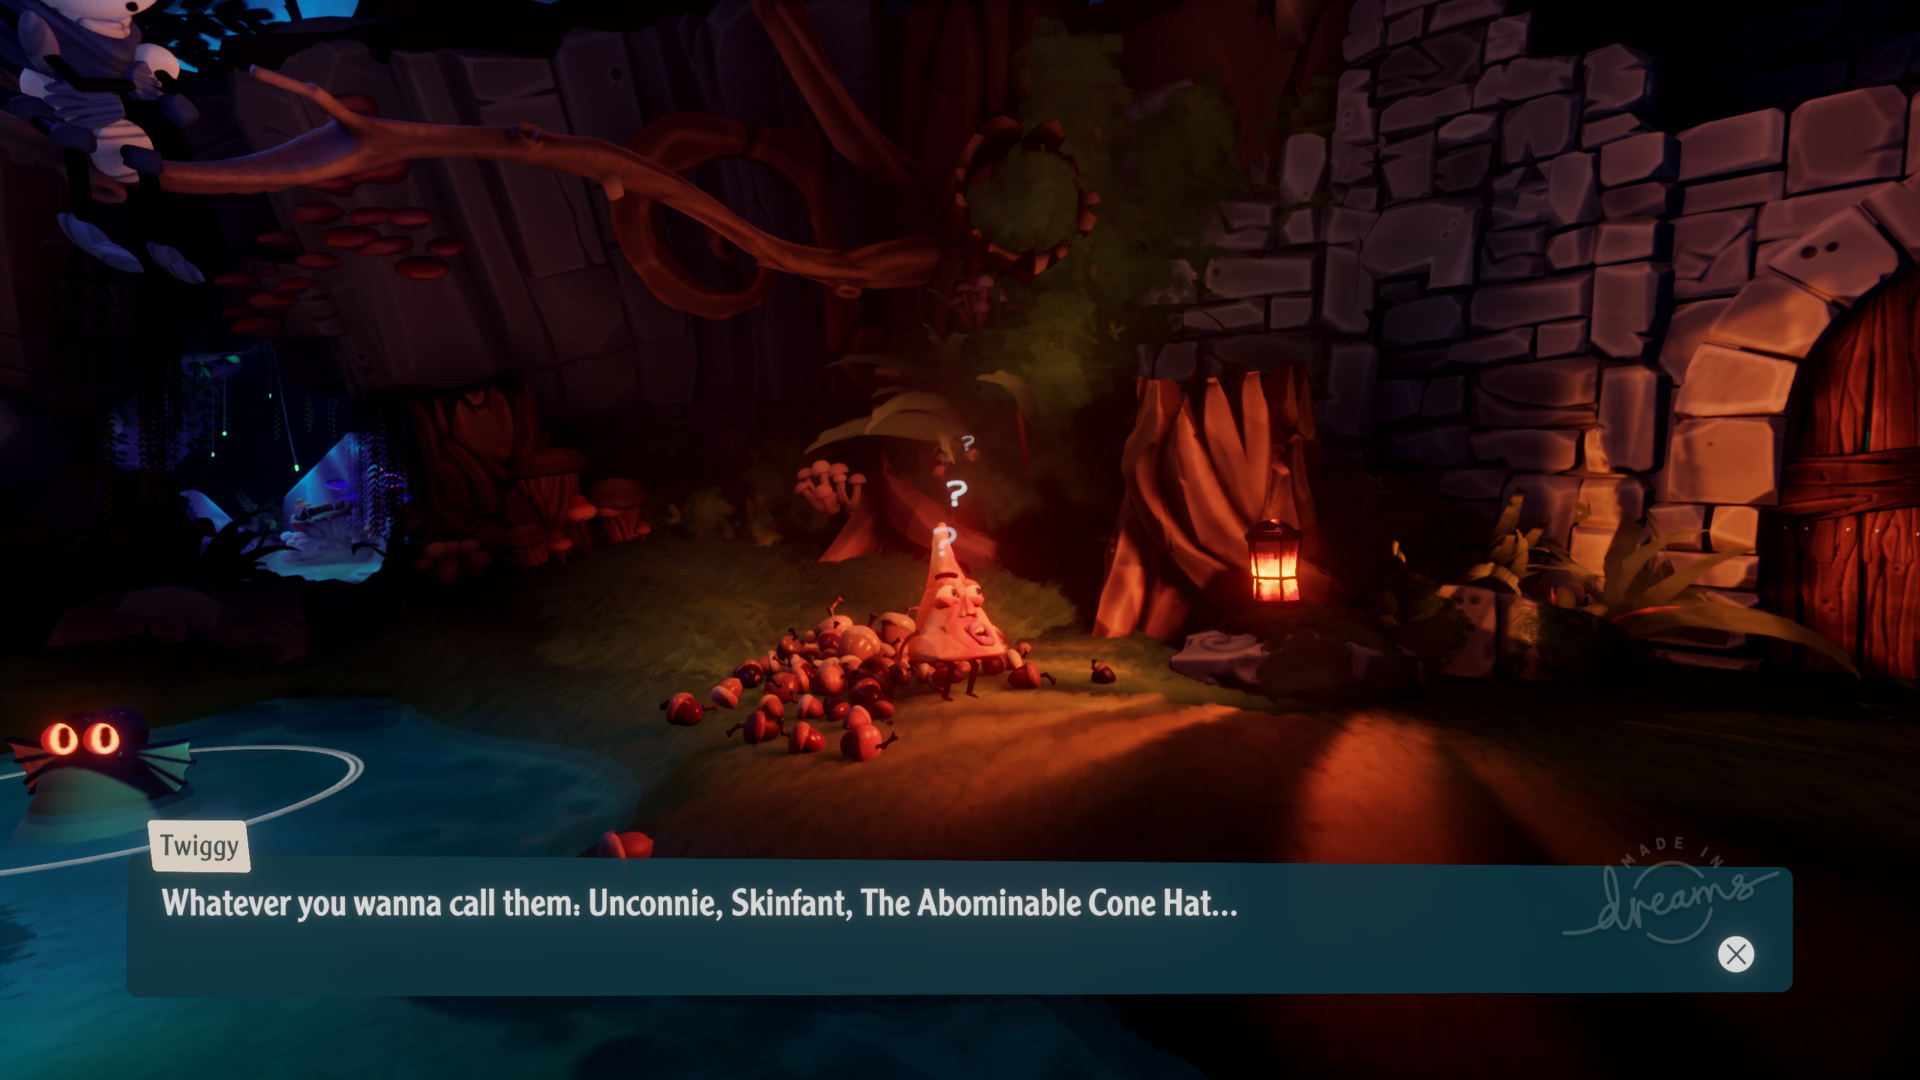
\includegraphics[width = 0.5\textwidth]{Imagenes/OCR/Boc2.png}
		\caption{Ejemplo imagen de texto en bocadillos con poca diferenciación con el fondo }
	\end{figure}
\end{enumerate} 

\subsection{Preprocesamiento de imágenes}
\footnote{(Image Processing in OpenCV)\url {https://docs.opencv.org/4.x/d2/d96/tutorial_py_table_of_contents_imgproc.html}}
El preprocesamiento de imágenes consiste en aplicar técnicas que modifican las imágenes para que sea más fácil de reconocer por una OCR el texto existente.
Para saber que técnicas mejora el reconocimiento y baja el CER, se ha ido probando con cada una de ellas, obteniendo los resultados e identificando aquellas técnicas que ayuda a mejorar el CER medio.
Las técnicas probadas son las siguientes:

\begin{enumerate}
	\item Escala de grises:
	Convierte una imagen a un formato de un solo canal, representando solo la intensidad de luz. Es útil para simplificar y reducir la cantidad de datos cuando el color no es relevante.
	\begin{figure}[H]
		\centering
		
\includegraphics[width = 0.5\textwidth]{Imagenes/Preprocesado/1.png}
	\end{figure}
	\item Aumentar contraste: 
	Mejora la diferencia entre las áreas claras y oscuras en una imagen, lo que facilita la detección de detalles.
		\begin{figure}[H]
		\centering
		
\includegraphics[width = 0.5\textwidth]{Imagenes/Preprocesado/2.png}
	\end{figure}
	\item Ecualización del histograma:
	Ajusta el contraste de la imagen extendiendo la distribución de los niveles de gris, mejorando el rango dinámico y resaltando los detalles.
		\begin{figure}[H]
		\centering
		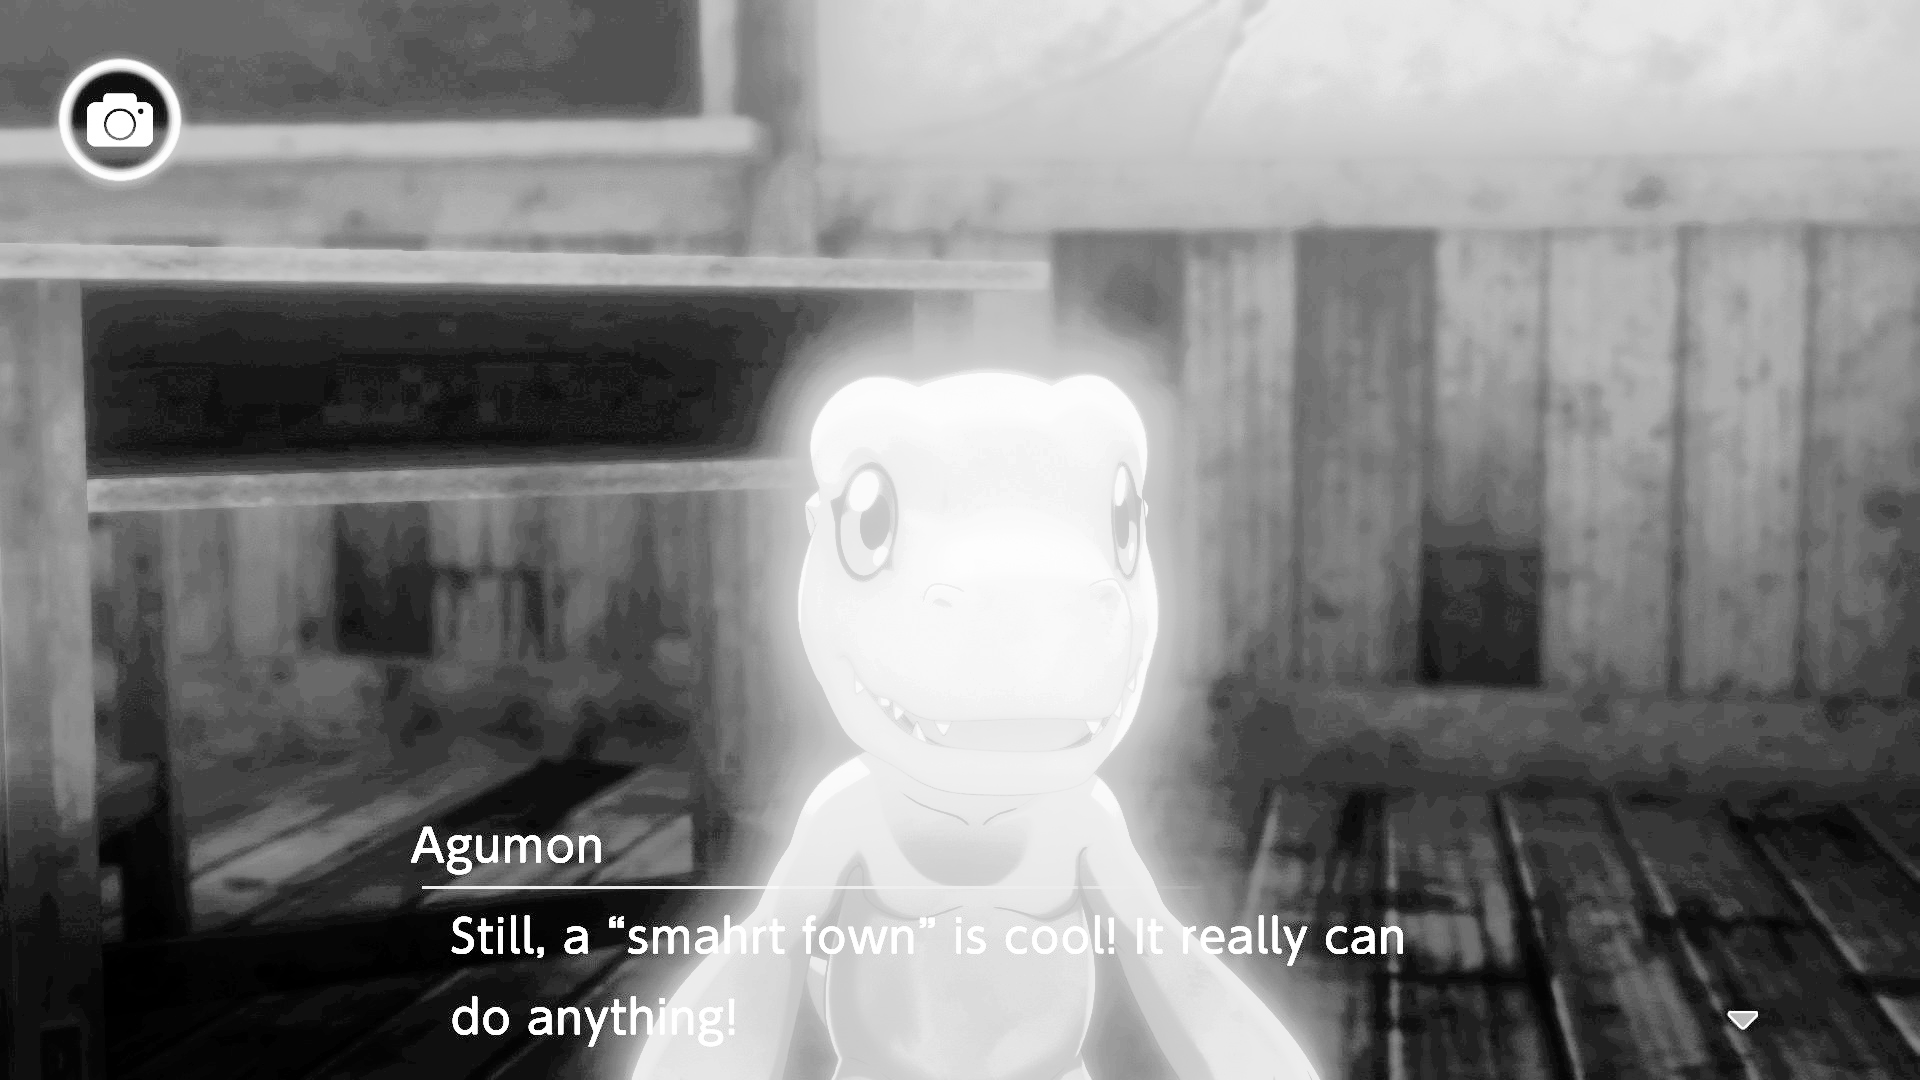
\includegraphics[width = 0.5\textwidth]{Imagenes/Preprocesado/3.png}
	\end{figure}
	
	\item Corrección del gamma:
	Ajusta los valores de intensidad en la imagen para compensar la percepción humana y los errores del sensor, lo que puede hacer que ciertas áreas sean más visibles.
		\begin{figure}[H]
		\centering
		
\includegraphics[width = 0.5\textwidth]{Imagenes/Preprocesado/4.png}
	\end{figure}
	
	\item Filtro de nitidez: 
	Realza los bordes de una imagen para destacar detalles, útil en aplicaciones donde se requiere mayor definición.
		\begin{figure}[H]
		\centering
		
\includegraphics[width = 0.5\textwidth]{Imagenes/Preprocesado/5.png}
	\end{figure}
	
	\item Adaptive Thresholding:
	Segmenta una imagen dividiéndola en áreas claras y oscuras, aplicando un umbral que se ajusta de forma adaptativa a las variaciones locales de luz.
		\begin{figure}[H]
		\centering
		
\includegraphics[width = 0.5\textwidth]{Imagenes/Preprocesado/6.png}
	\end{figure}
	
	\item Simple Thresholding: 
	Asigna un valor binario a cada píxel dependiendo de si está por encima o por debajo de un umbral específico, útil para crear máscaras y segmentación sencilla.
		\begin{figure}[H]
		\centering
		
\includegraphics[width = 0.5\textwidth]{Imagenes/Preprocesado/7.png}
	\end{figure}
	
	\item Image Blurring (Desenfoque de Imagen): 
	Reduce el ruido y los detalles mediante técnicas como filtros Gaussianos o de promediado, comúnmente utilizado para suavizar imágenes antes de un análisis.
		\begin{figure}[H]
		\centering
		
\includegraphics[width = 0.5\textwidth]{Imagenes/Preprocesado/8.png}
	\end{figure}
	
	\item Redimensionar la imagen: 
	Cambia las dimensiones de una imagen, lo que puede ser útil para normalizar entradas a una red neuronal o ajustar el tamaño de una imagen para procesamiento.
		\begin{figure}[H]
		\centering
		
\includegraphics[width = 0.5\textwidth]{Imagenes/Preprocesado/9.png}
	\end{figure}
		
	\item Dilatar y erosionar: 
	Técnicas de morfología matemática que expanden o reducen las regiones blancas (o los objetos) en una imagen binaria, útiles para limpieza de ruido o cierre de contornos.
		\begin{figure}[H]
		\centering
		
\includegraphics[width = 0.5\textwidth]{Imagenes/Preprocesado/10.png}
	\end{figure}
	
	\item Denoising (Reducción de ruido): 
	Elimina o reduce el ruido en una imagen para mejorar la calidad visual y el rendimiento de tareas de reconocimiento.
		\begin{figure}[H]
		\centering
		
\includegraphics[width = 0.5\textwidth]{Imagenes/Preprocesado/11.png}
	\end{figure}
	
\end{enumerate}
Resultados obtenidos con los distintos tipos de preprocesamiento en cada categoría de imágenes.
\begin{table}[H]
	\begin{tabular}{llllll}
		Tipo                                                                 & Complejo                      & Simple                       & PixelArt                      & TxTBoc                       & TxtBoc2                       \\
		Grises                                                               & 3.72                          & 0.59                         & 2.69                          & 1.17                         & 2.16                          \\
		Contraste                                                            & 5.06                          & 0.81                         & 2.39                          & 1.13                         & 10.07                         \\
		\begin{tabular}[c]{@{}l@{}}Ecualización\\ de histograma\end{tabular} & 5.59                          & 3.60                         & 6.56                          & 2.41                         & 8.67                          \\
		Gamma                                                                & 3.72                          & 0.59                         & 2.69                          & 1.17                         & 2.16                          \\
		Filtro de nitidez                                                    & 11.06                         & 2.17                         & 8.84                          & 3.29                         & 12.05                         \\
		Thresholding C                                                       & \cellcolor[HTML]{FF0000}16.80 & \cellcolor[HTML]{FF0000}9.44 & 10.36                         & 4.08                         & \cellcolor[HTML]{FF0000}23.44 \\
		\begin{tabular}[c]{@{}l@{}}Thresholding\\ Gaussian\end{tabular}      & 12.85                         & 9.35                         & \cellcolor[HTML]{FF0000}16.16 & \cellcolor[HTML]{FF0000}4.71 & 22.83                         \\
		Thresold Binary                                                      & 4.05                          & \cellcolor[HTML]{00FF00}0.49 & 2.14                          & 1.79                         & 2.04                          \\
		\begin{tabular}[c]{@{}l@{}}Redimension\\ x1.5\end{tabular}           & 4.77                          & 0.80                         & 2.86                          & 1.27                         & 3.07                          \\
		Gaussian Blur                                                        & 3.02                          & 0.68                         & 2.34                          & 1.14                         & 1.86                          \\
		Median Blur                                                          & 2.75                          & 0.51                         & 2.75                          & 1.25                         & 1.37                          \\
		2 Blur                                                               & 2.26                          & 0.59                         & 2.15                          & 1.22                         & \cellcolor[HTML]{00FF00}1.09  \\
		Dilatación y erosión                                                 & 2.19                          & 0.51                         & 2.48                          & \cellcolor[HTML]{00FF00}0.69 & 1.83                          \\
		Dilatación                                                           & \cellcolor[HTML]{00FF00}1.80  & 0.62                         & \cellcolor[HTML]{00FF00}1.23  & 0.80                         & 5.53                          \\
		Erosión                                                              & 2.02                          & 1.00                         & 2.57                          & 0.82                         & 1.21                          \\
		Denoising                                                            & 3.23                          & 0.57                         & 2.64                          & 1.07                         & 1.70                         
	\end{tabular}
\end{table}

El CER en este caso supera al 1 debido a que el OCR reconoce más caracteres de lo que hay en el ground-truth, es decir, reconoce muchos caracteres "basura".

Se marca en rojo aquel tipo de preprocesamiento que da peor resultado en la categoría y en verde, aquel que da mejor resultado.

Obteniendo esta tabla y viendo los resultados de imágenes se ha ido probando distintas combinaciones de preprocesados de imágenes y se ha obtenido la siguiente combinación:
\begin{itemize}
	\item Grises
	\item Escalado
	\item Simple Threshold
	\item Denoising
	\item Blurring
	\item Dilate\_Erode	
\end{itemize}
Obteniendo estos resultados:
\begin{table}[H]
	\begin{tabular}{lllll}
		Complejo & Simple & PixelArt & TxTBoc & TxtBoc2                      \\
		2.57     & 0.29   & 2.01     & 1.01   & 1.49
	\end{tabular}
\end{table}
\subsection{Eliminación de caracteres basura}
Una posible salida de la OCR puede ser la siguiente:

\begin{verbatim}
	YRNY L., R Y .
	t ::;h.'. . ,’_:“?; -' [
	Y& i AT
	A DU T AR BIE
	e vl e \-' .: ’4 -7
	g ... . ‘s "
	_-'.‘_;g ""M“ a DO .
	* v o ‘ >
	e \1 v we » r
	—,:)‘“ - ~ ‘ S " v - .
	- ’ p S A ’ -t » e . -~
	) p '_" - Y . 4 ) ) e “ ",
	RS g~ C okl A e .
	o “\ ., ":.-.. _x '.- - — "- : ' . 1'1 N .»rv
	TN A foow. TREELYS 4 e
	v\ U - ' b.""*— .
	. . ) . ‘ . J - . h v ’k‘ Py
	Mo . : . ¢ . . . .
	. ’/. . A.; ‘-\ ' .
	it - g 03: b 4
	7 - ] > I »“ Y “. Pl
	L It's been a long road. You have the right to stretch your legs!
	L2 p
	’ - . r £ . R ¥ h N\
	y /’ - . J ’ ‘- - .i;" N
	
\end{verbatim}
Donde la frase que realmente importa es solamente una o dos líneas de la salida
\begin{verbatim}
		L It's been a long road. You have the right to stretch your legs!
\end{verbatim}
Esto es un problema importante que debemos solucionar ya que es imposible saber si un test es correcto o no con esta entrada.

En esta sección se propone una solución a este problema de caracteres ``basura'' usando el algoritmo\footnote{(Algoritmo para C++ Levenshtein distance)\url{https://github.com/guilhermeagostinelli/levenshtein/blob/master/levenshtein.cpp}} de distancia \emph{levenshtein}.

La distancia de Levenshtein\footnote{(Levenshtein distance Wikipedia) \url{https://en.wikipedia.org/wiki/Levenshtein_distance} } (también conocida como distancia de edición) es una métrica utilizada para medir el grado de diferencia entre dos cadenas de texto. Específicamente, se define como el número mínimo de operaciones necesarias para transformar una cadena en otra, utilizando tres tipos de operaciones básicas:
\begin{itemize}
	\item Inserciones: Agregar un carácter.
	\item Eliminaciones: Eliminar un carácter.
	\item Sustituciones: Reemplazar un carácter por otro.
\end{itemize}

Suponiendo que tenemos el texto esperado de la imagen,  utilizando esta métrica, podemos obtener la distancia levenshtein entre una línea del texto esperado y una línea del texto reconocido por la OCR. Con la distancia obtenida y aplicando un cierto umbral, podemos identificar aquellas líneas que más se asimila al texto esperado, obteniendo así las líneas deseadas y descartando aquellas que no cumpla un cierto umbral.

Uno de los resultados obtenidos aplicando la distancia levenshtein es la siguiente:
\begin{itemize}
	\item Texto esperado:
	
	\begin{verbatim}
		Agumon
		Still,a "smahrt fown" is cool! It really can
		do anything!
	\end{verbatim}
	\item Texto real de OCR:
	
		\begin{verbatim}
	"
	|
	\ J
	—
	Agumon /
	Still, a “smahrt fown” is cool! It really can
	do anything! <
	\end{verbatim}
	\item Texto aplicando distancia levenshtein:
	\begin{verbatim}
	Agumon Still smahrt fown is cooll It really can do anything
	\end{verbatim}
\end{itemize}  
Obteniendo estos nuevos resultados en el CER medio:

\begin{table}[H]
	\begin{tabular}{llllll}
		Tipo        & Complejo & Simple & PixelArt & TxTBoc & TxtBoc2                      \\
		OCR         & 2.57     & 0.29   & 2.01     & 1.01   & \cellcolor[HTML]{FFFFFF}1.49 \\
		Levenshtein & 0.63     & 0.16   & 0.63     & 0.55   & 0.42                        
	\end{tabular}
\end{table}
\section{Descripción de los tests}
\subsection{Testing sobre errores de cadena no localizada - detección de placeholder}
\begin{itemize}
	\item Problema: \\
	Sucede cuando el texto incluye placeholders de variables p.ej \{name\}  \\
	\item Entrada: \\
	Cadena leída por el detector de texto \\
	Marcadores de placeholder \\
	\item Comportamiento: \\
	El test asume que los marcadores de placeholder no se usan de manera natural en el lenguaje escrito.
	Lo que hará el test es leer la string de entrada y contar el número de caracteres hasta que aparezca un marcador de inicio de placeholder. En ese momento se guardará el número de caracteres hasta esa primera aparición, y después guardará la string que aparece de ese momento hasta que se encuentre un marcador de cierre de placeholder. 
	Al final, el test escribirá en pantalla el número del carácter en el que empieza cada placeholder y la cadena de texto que haya dentro de dicho placeholder.
\end{itemize}

\subsection{Testing sobre problema de fuente
}
\begin{itemize}
	\item Problema: \\
	La fuente utilizada no incluye alguno de los caracteres especiales de un idioma , por ejemplo las tildes (á) , la ñ en español.  \\
	\item Entrada: \\
	Cadena leída por el detector de texto
	
	Cadena de texto esperado
	
	\item Comportamiento: \\
	El test leerá la cadena de texto leída por el detector y las compara uno a uno con la cadena de texto esperado , se guardará la posición en la que son distintos y se mostrará en la salida el número de caracteres distintos y su posición.
	
\end{itemize}



\subsection{Testing sobre cadena de texto no localizada}
\begin{itemize}
	\item Problema: \\

	\item Entrada: \\

	\item Comportamiento: \\

\end{itemize}
\subsection{Testing sobre solapamiento de texto}

\begin{itemize}
	\item Problema: \\
	Cuando el texto escrito es más largo de lo esperado por el programador por lo que se sale de los límites del espacio guardado para ese texto y se solapan. \\
	\item Entrada: Imagen\\
	
	\item Comportamiento: Para resolver este problema se platea usar el OCR para detectar las posiciones de los textos , seguido de una librería gráfica para detectar el contorno de la caja delimitadora guardado para ese texto, y obtener así sus posiciones. Comparando la posición del texto y la posición de la caja delimitadora obtenemos si el texto se está saliendo de la caja o no.\\
	Para simplificar el test , damos algunas restricciones: 
	\begin{itemize}
		\item En la imagen , el texto tiene que aparecer completamente en horizontal sin ninguna rotación sobre el eje x.
		\item Detectamos de primeras texto que se sobresale por los lados.
		\item Al ser un botón , tiene que estar resaltado , un claro contraste con el fondo y el texto para facilitar la detección
		\item Debe tener una forma de caja o ventana(cuadriculada, cuadriculada redondeada), no vale por ejemplo un bocadillo en forma de nube.
	\end{itemize} 
	
\end{itemize}
\subsection{Testing sobre truncamiento de texto
}
\begin{itemize}
	\item Problema: \\
	
	\item Entrada: \\
	
	\item Comportamiento: \\
	
\end{itemize}
\subsection{Testing sobre error tipográfico/gramatical
}
\begin{itemize}
	\item Problema: \\
	
	\item Entrada: \\
	
	\item Comportamiento: \\
	
\end{itemize}
 


\chapter{Implementación de la herramienta}
\label{cap:implementacion}

Como se ha hecho la herramienta y sus partes

\section{Implementación de los tests}
\subsection{Test sobre solapamiento de texto}
\chapter{Evaluación de la herramienta}
\label{cap:evaluacion}

En este capítulo se describirá la evaluación de la herramienta separando en una evaluación para el módulo de OCR, otra para el módulo de tests y una evaluación de la herramienta de forma conjunta(end to end testing).
En la parte de OCR se evaluará la librería utilizada, la mejora que proporciona la parte de preprocesamiento y la limpieza de caractéres basura utilizando distancia Levenshtein.
En la parte de tests se evaluará la precisión de los tests asegurándonos de que no exista casos que de un falso error en el test. 
De forma genérica se evaluará la herramienta con los resultados obtenidos ejecutando la herramienta midiendo la precisión.

\section{Pruebas y resultados de los OCR}
\label{sec:Evaluación_OCR}
En esta sección se hará una evaluación de los distintos OCRs para elegir la más conveniente para nuestra herramienta.
La evaluación se hará sobre las librerías de Tesseract, EasyOCR y OCRopus, son estas elegidas por su disponibilidad gratuita.

El objetivo de la evaluación es elegir el OCR que mejor se adapte a nuestras necesidades, lo que resalta la importancia de la precisión del OCR.
Para poder medir esa precisión, tendremos en cuenta el CER(\textit{Character Error Rate}). Además el tiempo también es un factor importante que tendremos en cuenta.

El CER(\textit{Character Error Rate}) es una métrica usada comúnmente para evaluar la precisión de un sistema de reconocimiento de caracteres u otros sistemas que transcriba texto. El valor se obtiene calculando el número de errores a nivel de carácter dividido por el número total de caracteres en el texto de referencia.
Los errores pueden ser debidos a:
\begin{enumerate}
	\item Sustituciones: Un carácter incorrecto reemplaza a uno correcto.
	\item Inserciones: Aparece un carácter extra que no debería estar.
	\item Eliminaciones: Falta un carácter que debería estar presente.
\end{enumerate}
La fórmula general para calcular el CER es:

$CER = \frac{S+D+I}{N} $ 

Donde:

S es el número de sustituciones.

D es el número de eliminaciones.

I es el número de inserciones.

N es el número total de caracteres en el texto de referencia.

El CER se expresa como un valor entre 0 y 1 (o como porcentaje), donde 0 significa que no hubo errores (transcripción perfecta) y 1 (o 100) indica que todos los caracteres son incorrectos.

La metodología seguida para la evaluación es la siguiente:

\begin{enumerate}
	\item Se hará la evaluación de forma independiente con las 3 librerías de OCR. Tesseract, EasyOCR y OCRopus.
	\item Se ha elegido 13 imágenes nombrados del 1 al 13 siendo la imagen 1(figura \ref{fig:imagen1}) el más simple y el 13(figura \ref{fig:imagen13}) el más complejo. Para la clasificación de simplificad de las imágenes se ha tenido en cuenta el número de caracteres a reconocer y la complejidad del fondo, entre ellas, el contraste y el número de geometrías.
	Las imágenes se pueden encontrar en el repositorio del trabajo\footnote{Repositorio github con las imágenes de evaluación: \url{https://github.com/Dewo2000/TFG-2024-2025/tree/main/OCRTests/images}}.
\begin{figure}[h]
	\centering
	\begin{minipage}{0.45\textwidth}
		\centering
		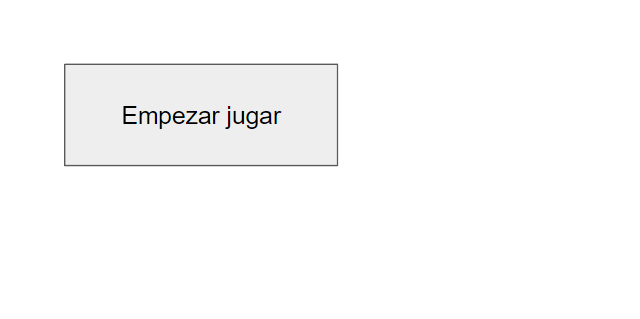
\includegraphics[width=\linewidth]{Imagenes/Evaluacion_OCR/1.png}
		\caption{Ejemplo de imagen simple.}
		\label{fig:imagen1}
	\end{minipage}
	\hfill
	\begin{minipage}{0.45\textwidth}
		\centering
		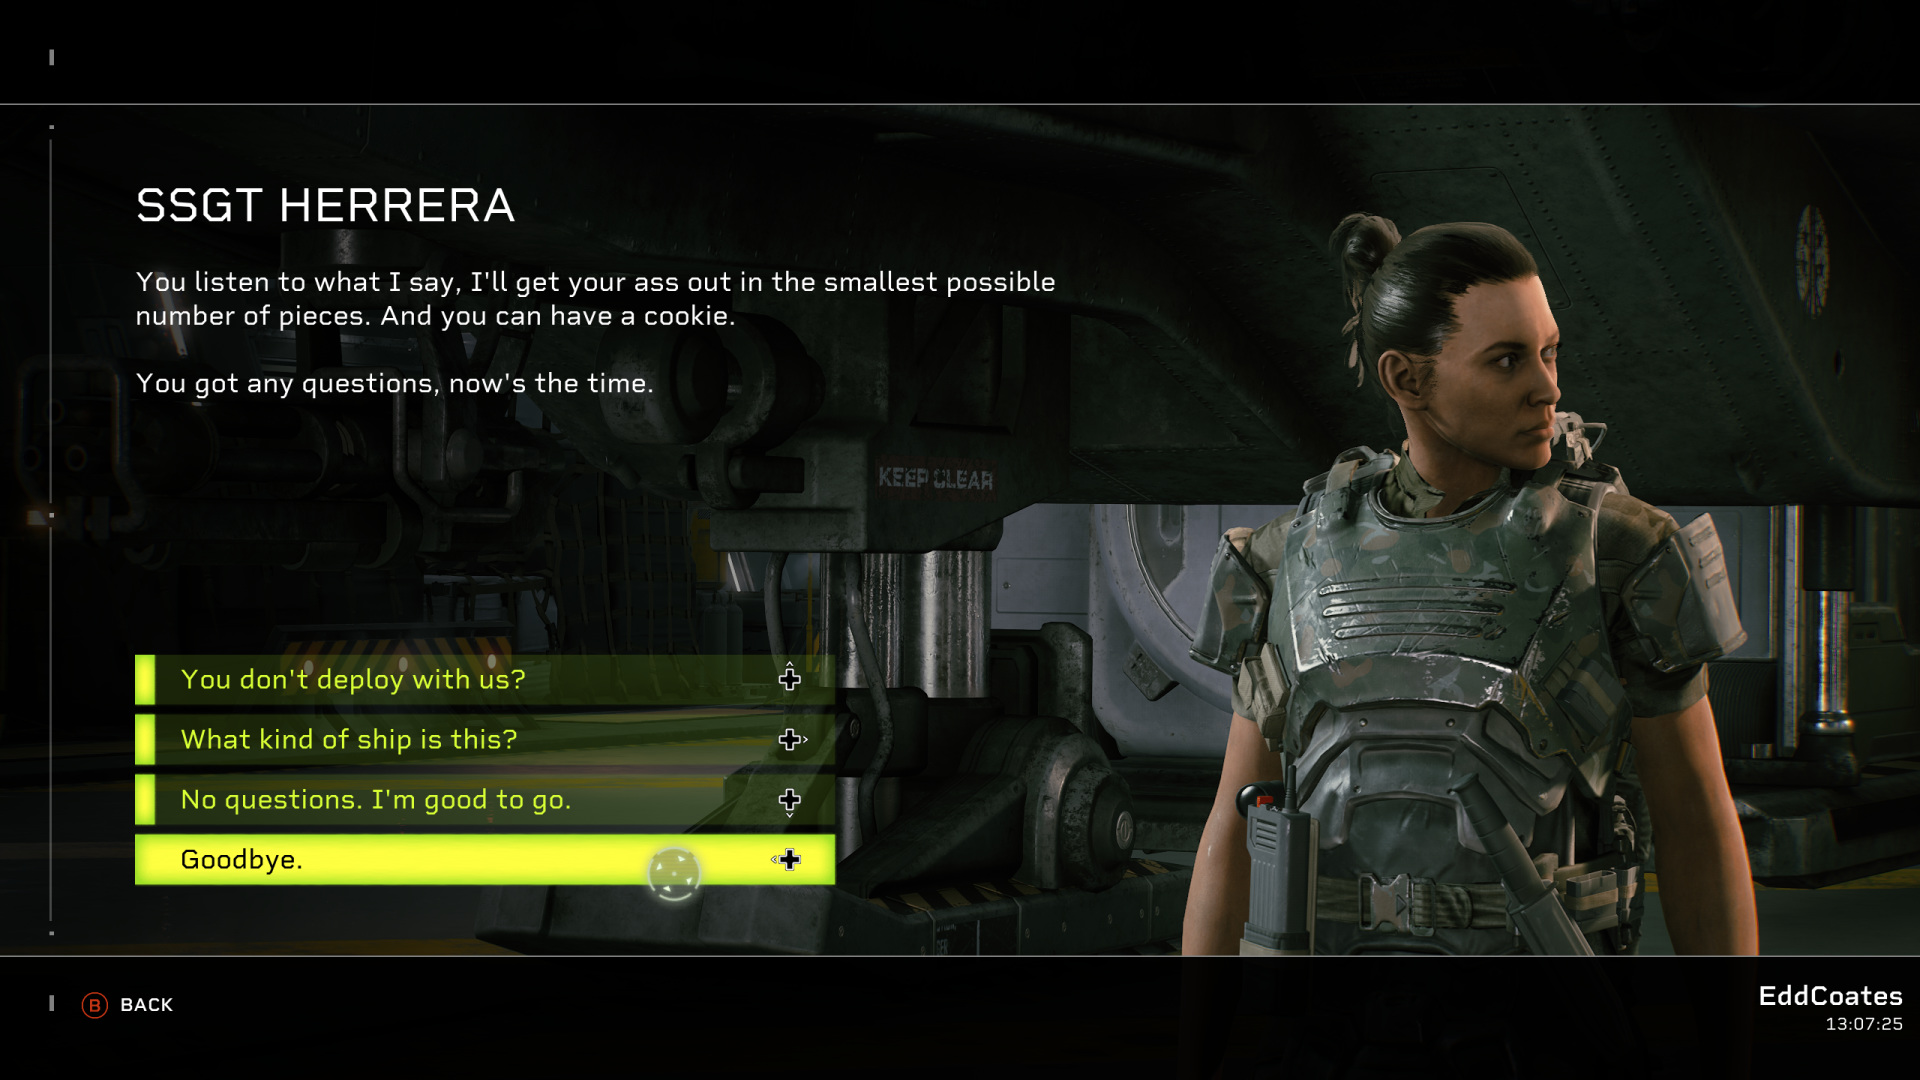
\includegraphics[width=\linewidth]{Imagenes/Evaluacion_OCR/13.png}
		\caption{Ejemplo de imagen complejo.}
		\label{fig:imagen13}
	\end{minipage}
\end{figure}
	\item Cada imagen será procesadas por el OCR utilizando el modelo por defecto de cada una de ellas.  
	\item Se utiliza la libreria Jiwer\footnote{(Jiwer Usage)\url {https://jitsi.github.io/jiwer/usage/}} en python para los cálculos de CER.
	\item Se ejecutará 6 veces el proceso de reconocimiento de cada OCR para sacar el tiempo medio de cada una.
\end{enumerate}


En los resultados de los OCR se encontrará un valor llamado CER medio, este valor se obtiene calculando el número total de errores a nivel de carácter encontrado en toda la batería de prueba divido entre el número total de caracteres de toda la batería de prueba.

Los resultados de los OCRs son las siguientes:
\begin{table}[H]
	\centering
	\caption{Resultado de CER de los OCR (Redondeado a 3 decimales)}
	\begin{tabular}{llll}
		\textbf{Imagen} & \textbf{Tesseract} & \textbf{EasyOCR} &\textbf{OCRopus} \\
		1  & 0.000 & 0.000 & 0.000 \\
		2  & 0.063 & 0.281 & 0.406 \\
		3  & 0.538 & 0.212 & 0.538 \\
		4  & 0.043 & 0.109 & 0.978 \\
		5  & 0.289 & 0.086 & 0.719 \\
		6  & 0.025 & 0.025 & 0.700 \\
		7  & 0.750 & 0.000 & 1.417 \\
		8  & 0.935 & 0.652 & 0.870 \\
		9  & 0.721 & 0.256 & 0.744 \\
		10 & 1.000 & 0.857 & 8.286 \\
		11 & 0.050 & 0.150 & 2.550 \\
		12 & 0.352 & 0.055 & 0.834 \\
		13 & 0.230 & 0.337 & 0.881 \\
		\textbf{CER medio} & \textbf{0.384}& \textbf{0.232} & \textbf{1.456}\\
	\end{tabular}
	\label{table:OCRResult}
\end{table}
\begin{table}[H]
	\centering
	\caption{Resultado de OCR en tiempo(ms)}
	\begin{tabular}{llll}
		\textbf{Iteración} & \textbf{Tesseract}& \textbf{EasyOCR}& \textbf{OCRopus} \\
		1  & 5539   & 204625 & 86213  \\
		2  & 5580   & 223809 & 90172  \\
		3  & 5539   & 216701 & 88290  \\
		4  & 5720   & 238900 & 83278  \\
		5  & 5602   & 216791 & 87810  \\
		6  & 5571   & 204502 & 88789  \\
		\textbf{Tiempo medio} & \textbf{5591}&\textbf{217554}&\textbf{87425} \\
	\end{tabular}
	\label{table:OCRResultTime}
\end{table}


Como podemos ver en la tabla \ref{table:OCRResult}, todos los OCRs han podido reconocer de forma exacta la imagen más simple y que todos han caido en la imagén 10. En cuanto las otras imágenes podemos observar que unas lo reconoce mejor Tesseract y otras EasyOCR por lo que ambos producen buenos resultados, en cuanto OCRopus, sus resultados ya no son tan buenos en comparación con las otras dos por lo que queda descartado. El OCR puede reconocer más caracteres del texto esperado por lo que el CER supera a 1 en algunos casos, lo llamamos caracteres basura que se explicará con más detalle en la sección \ref{subsec:Eliminación de caracter basura}. Aunque EasyOCR obtiene un mejor CER medio en los resultados (0.23) que Tesseract (0.38), Tesseract es muchísimo más rápido que EasyOCR teniendo un 211936 milisegundo de adelanto que equivale a 3 minutos y 50 segundos aproximadamente como podemos observar en la tabla \ref{table:OCRResultTime}. Por tanto decidimos seguir en adelante con Tesseract.



\section{Mejoras en el reconocimiento de texto en imágenes}
\label{sec:Mejoras en el reconocimiento}
Como podemos notar en los resultados del apartado anterior, la imagen 10 ha sido un reto para el CER de los OCRs, esto es debido a que el OCR reconoce como carácter geometrías del fondo y produce basura.Para solucionar esto, se plantea aplicar preprocesamiento a las imágenes y la limpieza del resultado usando distancia Levenshtein para mejorar la precisión del texto obtenido por el OCR disminuyendo el CER.

Para obtener más información sobre aquellos factores o características de las imágenes que puedan afectar al rendimiento y efectividad de la herramienta de OCR, se ha clasificado las imágenes en 5 categorías diferentes. La clasificación se ha hecho de forma subjetiva, de acuerdo a ciertas características de imágenes.
\begin{enumerate}
	\item Fondos simples(F.Simple)(Figura \ref{fig:Fsimple}). Imágenes donde la cantidad de geometrías del fondo son pocas o fáciles de reconocer(no se confunde con los caractéres).
	\begin{figure}[H]
		\centering
		
\includegraphics[width = 0.5\textwidth]{Imagenes/OCR/Simple.png}
		\caption{Ejemplo imagen fondos simples }
		\label{fig:Fsimple}
	\end{figure}
	
	\item Fondos complejos(F.Complejo)(Figura \ref{fig:Fcomplejo}). Imágenes donde la cantidad de geometrías del fondo son muchas o difíciles de reconocer(fácil de confundirse con los caractéres).
	\begin{figure}[H]
		\centering
		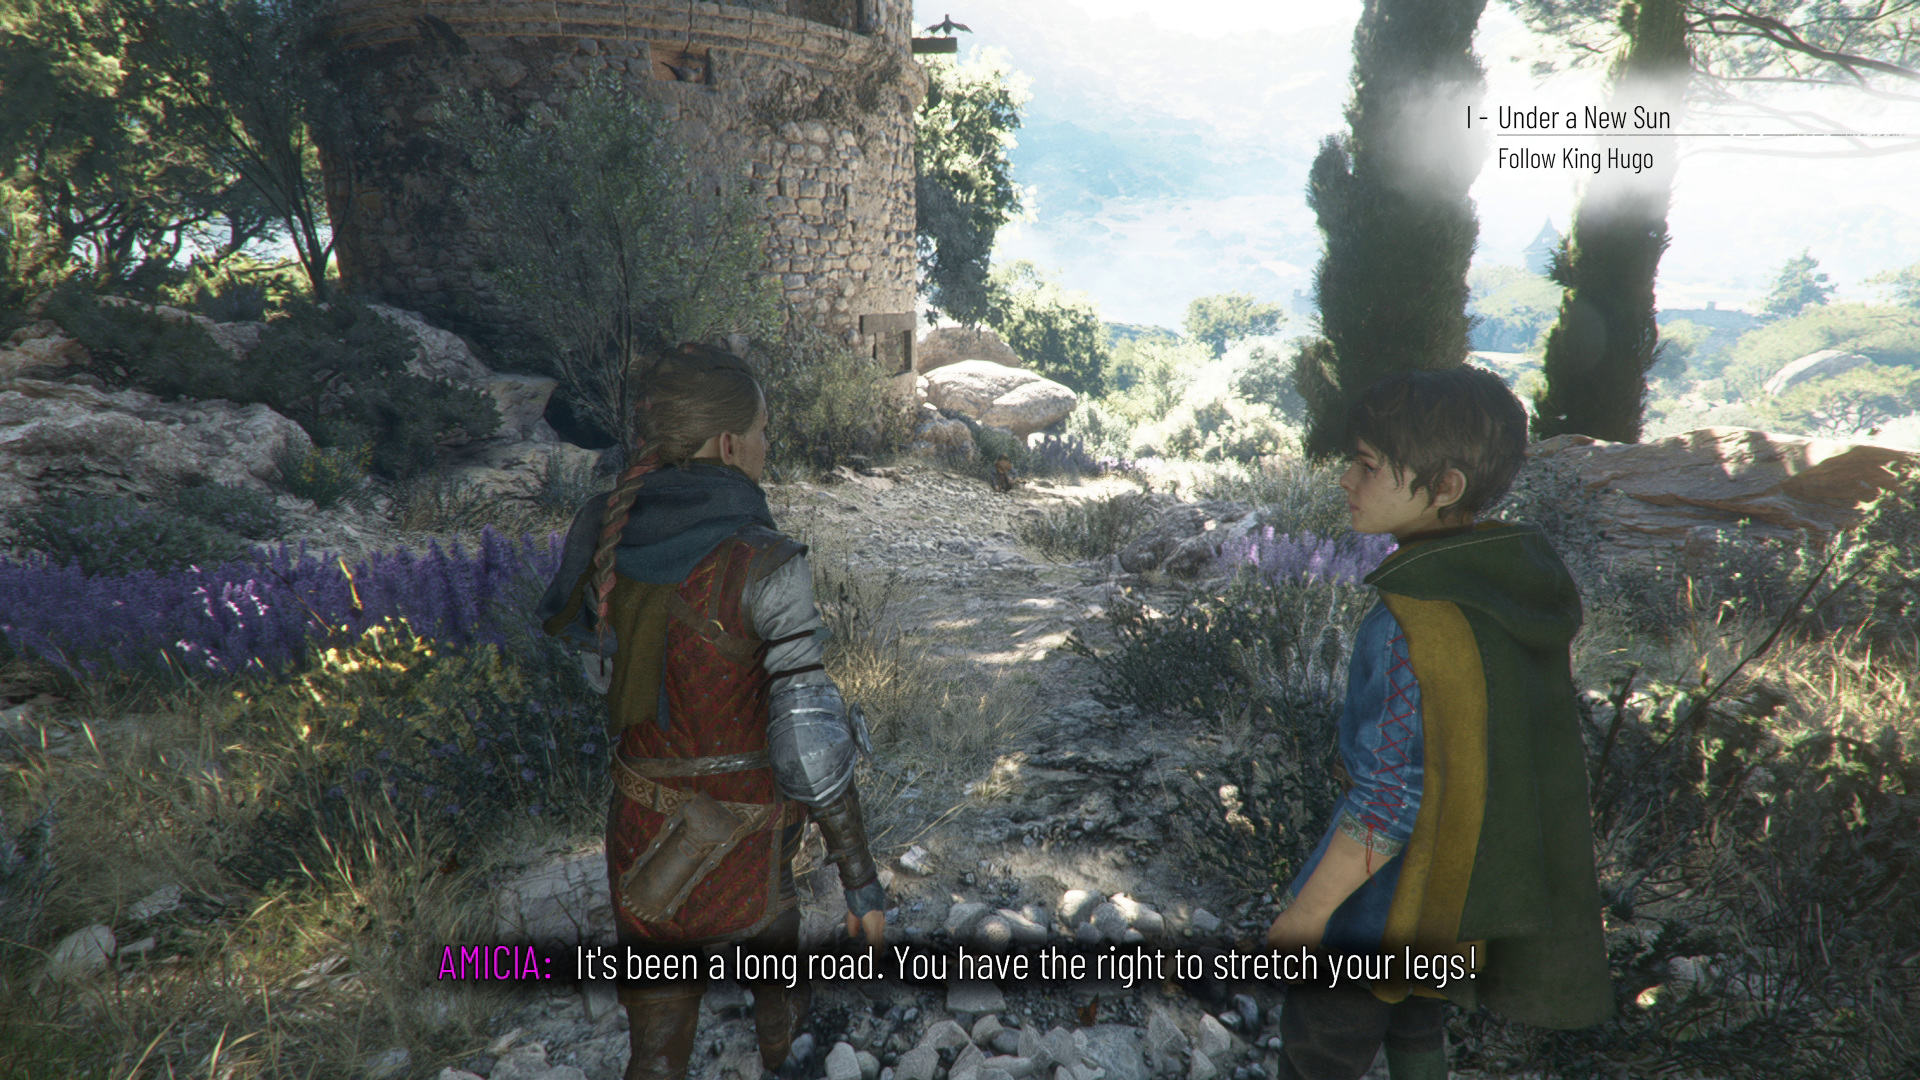
\includegraphics[width = 0.5\textwidth]{Imagenes/OCR/Complejo.png}
		\caption{Ejemplo imagen fondos complejos }
		\label{fig:Fcomplejo}
	\end{figure}
	\item PixelArt(PixelArt)(Figura \ref{fig:Pixelart}). Imágenes donde el fondo y las letras tiene un estilo pixelart. Como las imágenes son píxeladas(cuadrado de color que forman formas y texto), supone un reto para el OCR.
	\begin{figure}[H]
		\centering
		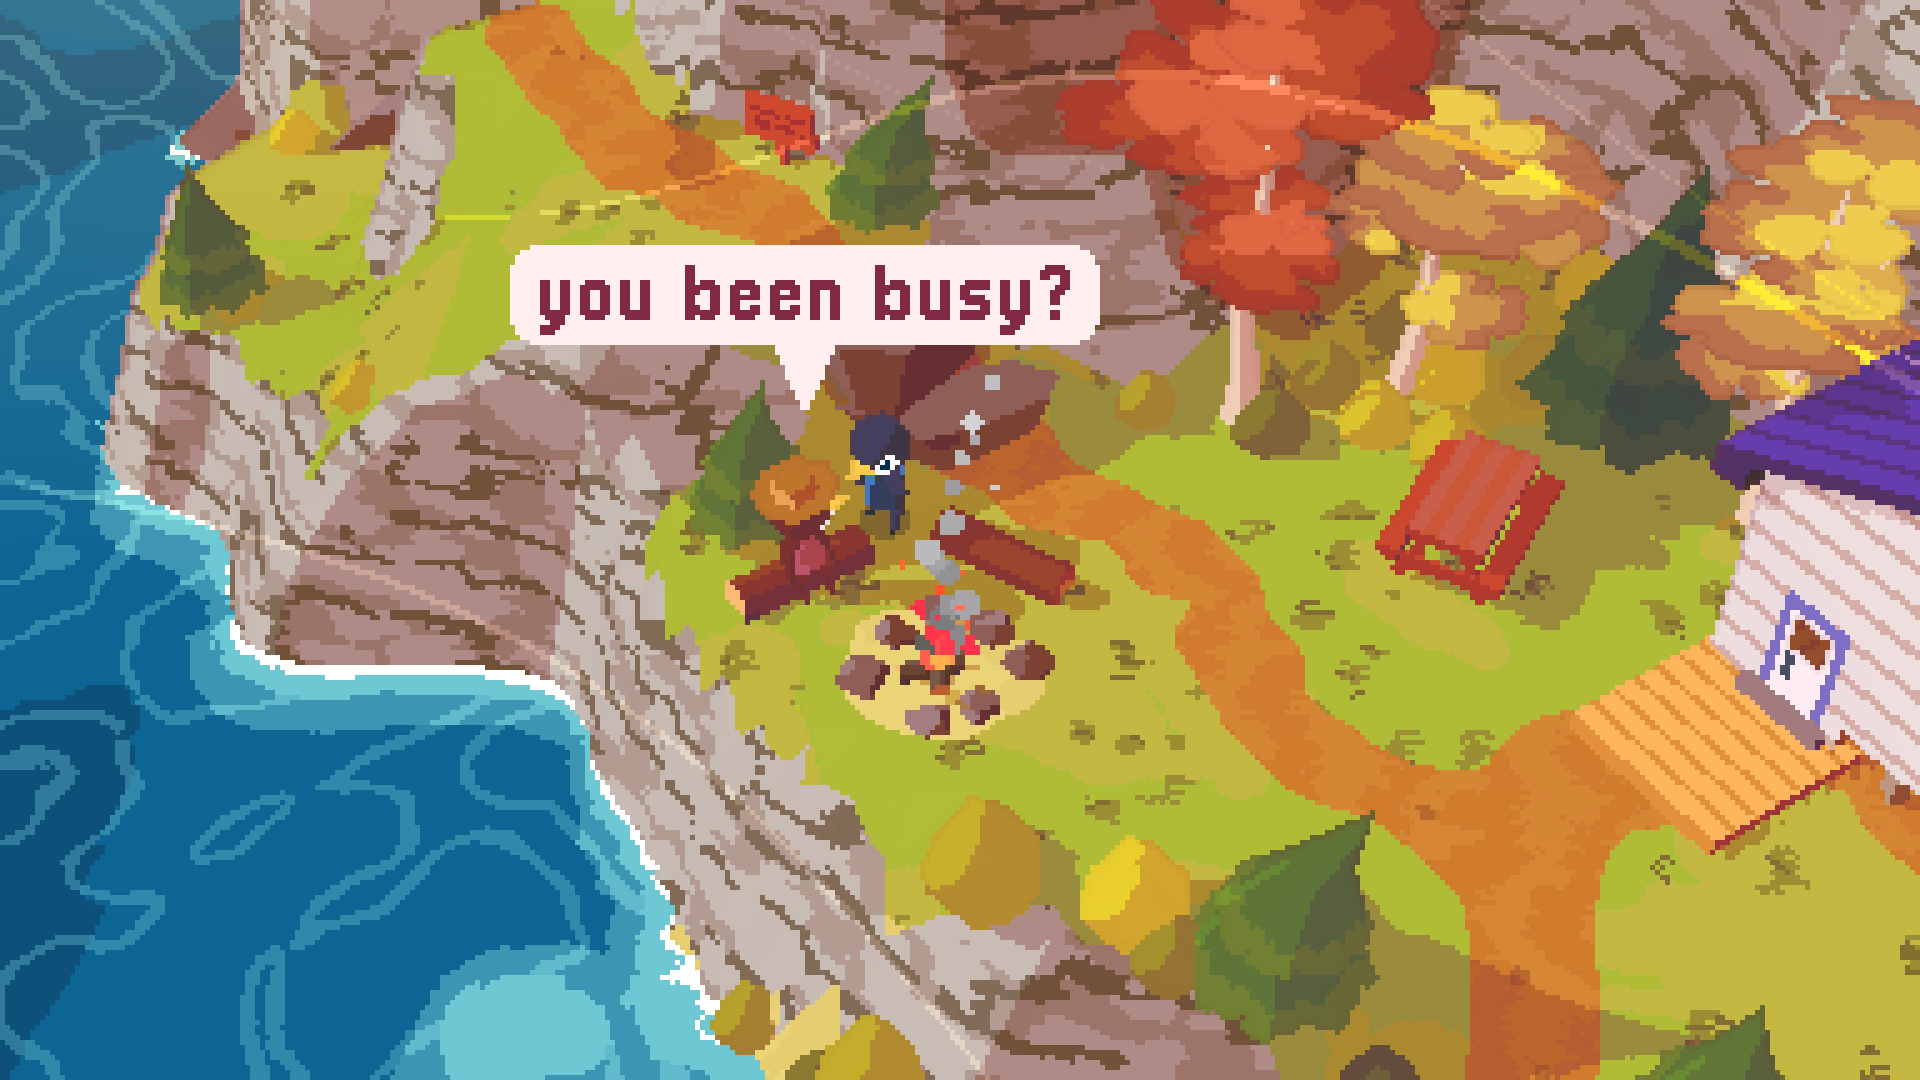
\includegraphics[width = 0.5\textwidth]{Imagenes/OCR/Pixel.png}
		\caption{Ejemplo imagen PixelArt }
		\label{fig:Pixelart}
	\end{figure}
	\item Texto en bocadillos(TxtBoc)(Figura \ref{fig:TxTBoc}). Imágenes donde el texto a reconocer se situa en un bocadillo y que el color del bocadillo tiene un alto contraste con el fondo.
	\begin{figure}[H]
		\centering
		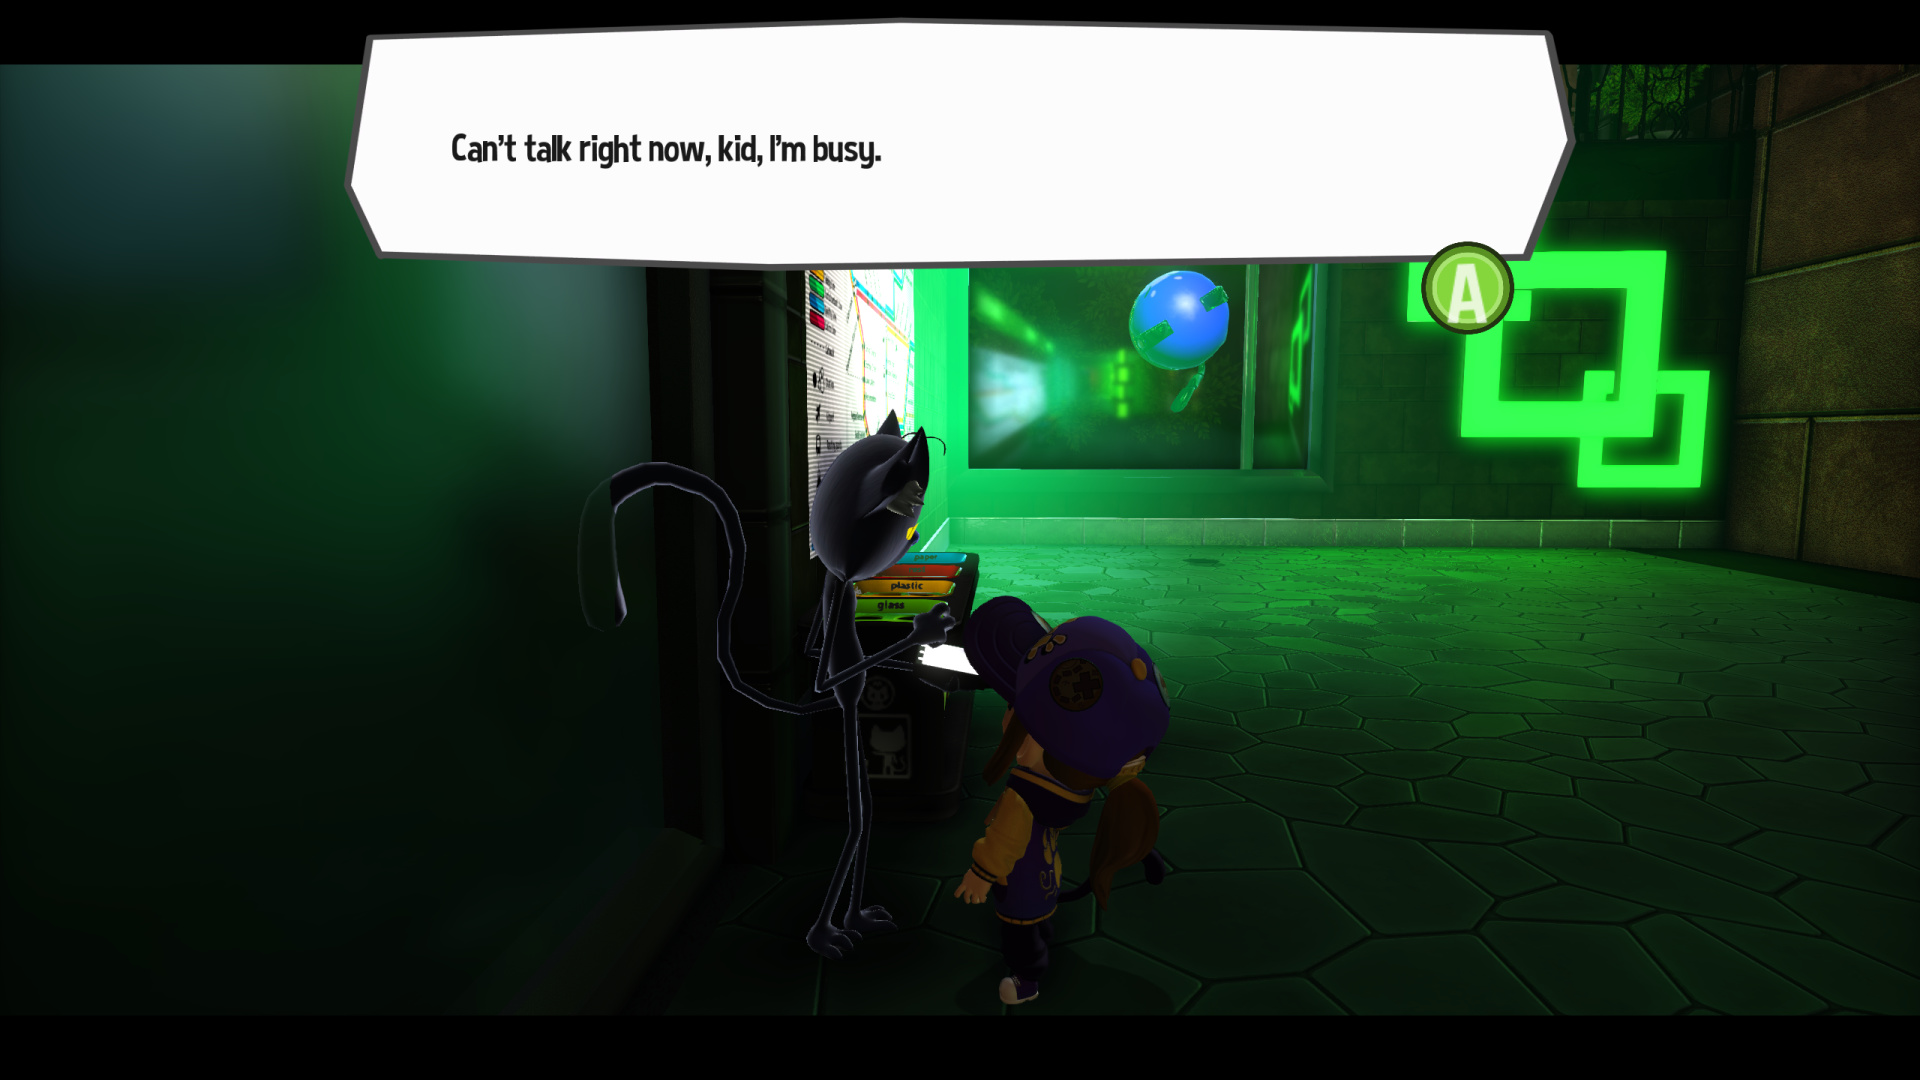
\includegraphics[width = 0.5\textwidth]{Imagenes/OCR/Boc.png}
		\caption{Ejemplo imagen de texto en bocadillo }
		\label{fig:TxTBoc}
	\end{figure}
	\item Texto en bocadillos con poca diferenciación con el fondo(TxtBoc2)(Figura \ref{fig:TxtBoc2}).Imágenes donde el texto a reconocer se situa en un bocadillo y que el color del bocadillo tiene un contraste medio o bajo con el fondo.
	\begin{figure}[H]
		\centering
		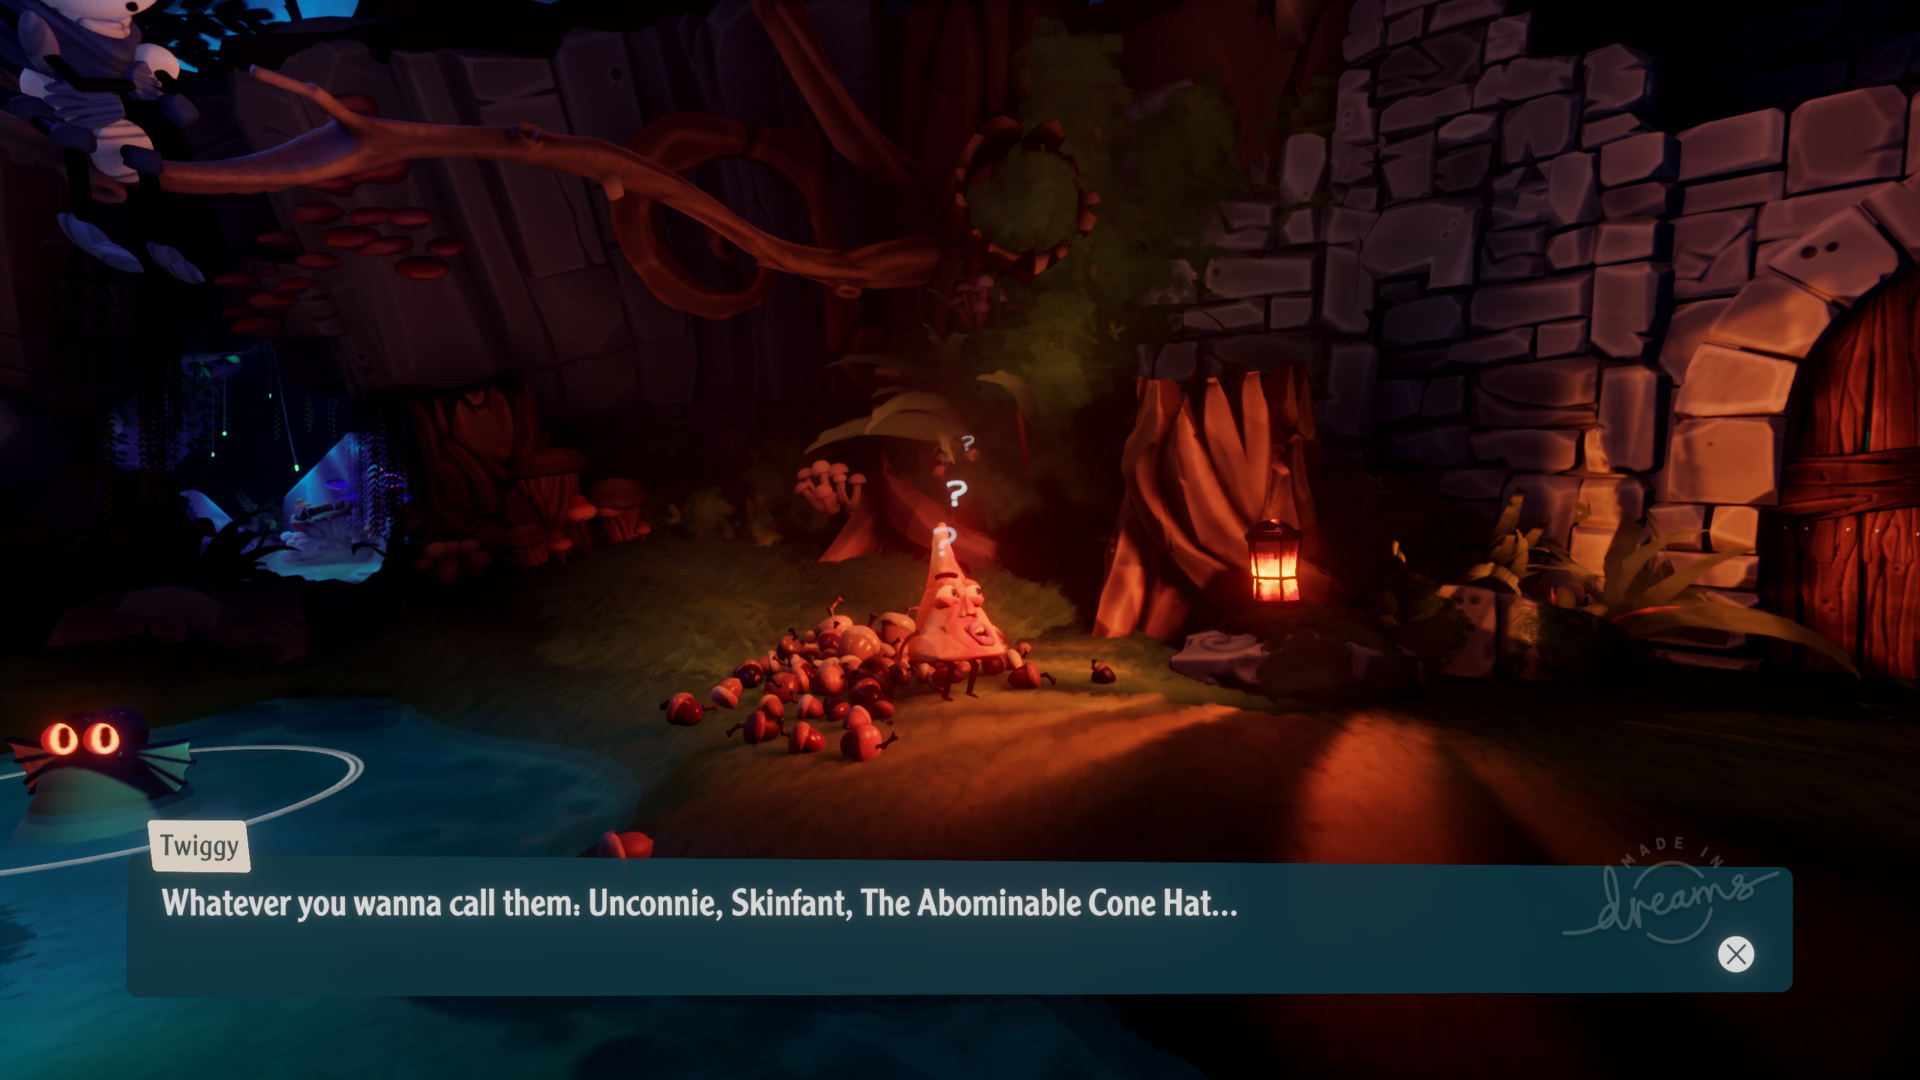
\includegraphics[width = 0.5\textwidth]{Imagenes/OCR/Boc2.png}
		\caption{Ejemplo imagen de texto en bocadillos con poca diferenciación con el fondo }
		\label{fig:TxtBoc2}
	\end{figure}
\end{enumerate} 


El preprocesamiento de imágenes consiste en aplicar técnicas que modifican las imágenes para que sea más fácil de reconocer por una OCR el texto existente.
Para saber que técnicas mejoran el reconocimiento, se ha ido probando con cada una de ellas en el manual de \cite{OpenCVProcessing}, obteniendo los resultados e identificando aquellas técnicas que ayuda a mejorar el CER medio.
Las técnicas probadas son las siguientes:

\begin{enumerate}
	\item Escala de grises(Figura \ref{fig:EscalaGrises}):
	Convierte una imagen a un formato de un solo canal, representando solo la intensidad de luz. Es útil para simplificar y reducir la cantidad de datos cuando el color no es relevante.
	\begin{figure}[H]
		\centering
		
\includegraphics[width = 0.5\textwidth]{Imagenes/Preprocesado/1.png}
		\caption{Imagen a escala de grises}
		\label{fig:EscalaGrises}
	\end{figure}
	\item Aumentar contraste(Figura \ref{fig:Contraste}): 
	Mejora la diferencia entre las áreas claras y oscuras en una imagen, lo que facilita la detección de detalles.
	\begin{figure}[H]
		\centering
		
\includegraphics[width = 0.5\textwidth]{Imagenes/Preprocesado/2.png}
		\caption{Imagen con aumento de contraste}
		\label{fig:Contraste}
	\end{figure}
	\item Ecualización del histograma(Figura \ref{fig:Histograma}):
	Ajusta el contraste de la imagen extendiendo la distribución de los niveles de gris, mejorando el rango dinámico y resaltando los detalles.
	\begin{figure}[H]
		\centering
		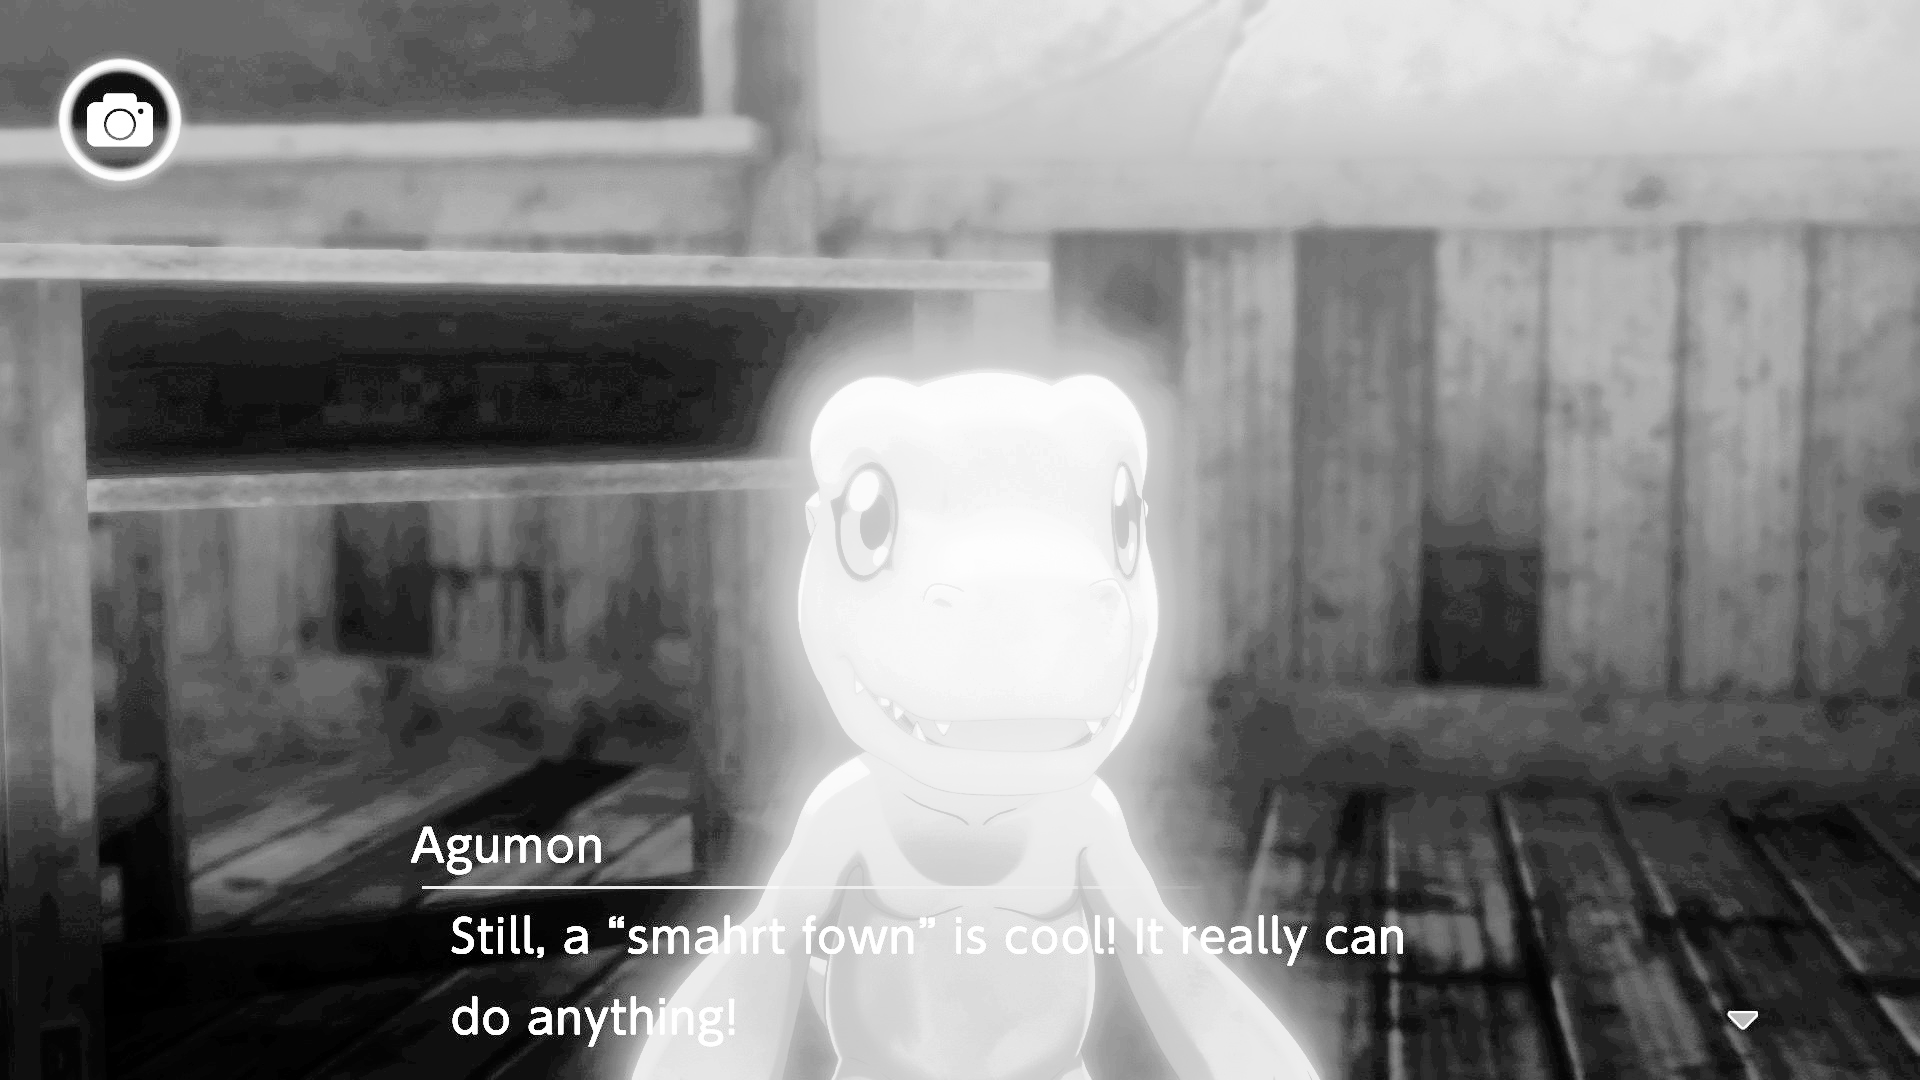
\includegraphics[width = 0.5\textwidth]{Imagenes/Preprocesado/3.png}
		\caption{Imagen con ecualización de histograma}
		\label{fig:Histograma}
	\end{figure}
	
	\item Corrección del gamma(Figura \ref{fig:Gamma}):
	Ajusta los valores de intensidad en la imagen para compensar la percepción humana y los errores del sensor, lo que puede hacer que ciertas áreas sean más visibles.
	\begin{figure}[H]
		\centering
		
\includegraphics[width = 0.5\textwidth]{Imagenes/Preprocesado/4.png}
		\caption{Imagen con corrección del gamma}
		\label{fig:Gamma}
	\end{figure}
	
	\item Filtro de nitidez(Figura \ref{fig:F.Nitidez}): 
	Realza los bordes de una imagen para destacar detalles, útil en aplicaciones donde se requiere mayor definición.
	\begin{figure}[H]
		\centering
		
\includegraphics[width = 0.5\textwidth]{Imagenes/Preprocesado/5.png}
		\caption{Imagen con filtro de nitidez}
		\label{fig:F.Nitidez}
	\end{figure}
	
	\item Adaptive Thresholding(Figura \ref{fig:Thresholding}):
	Segmenta una imagen dividiéndola en áreas claras y oscuras, aplicando un umbral que se ajusta de forma adaptativa a las variaciones locales de luz.
	\begin{figure}[H]
		\centering
		
\includegraphics[width = 0.5\textwidth]{Imagenes/Preprocesado/6.png}
		\caption{Imagen aplicando adaptive thresholding}
		\label{fig:Thresholding}
	\end{figure}
	
	\item Simple Thresholding(Figura \ref{fig:S.Threshold}): 
	Asigna un valor binario a cada píxel dependiendo de si está por encima o por debajo de un umbral específico, útil para crear máscaras y segmentación sencilla.
	\begin{figure}[H]
		\centering
		
\includegraphics[width = 0.5\textwidth]{Imagenes/Preprocesado/7.png}
		\caption{Imagen aplicando simple thresholding}
		\label{fig:S.Threshold}
	\end{figure}
	
	\item Image Blurring (Desenfoque de Imagen)(Figura \ref{fig:Blurring}): 
	Reduce el ruido y los detalles mediante técnicas como filtros Gaussianos o de promediado, comúnmente utilizado para suavizar imágenes antes de un análisis.
	\begin{figure}[H]
		\centering
		
\includegraphics[width = 0.5\textwidth]{Imagenes/Preprocesado/8.png}
		\caption{Imagen aplicando desenfoque de imagen}
		\label{fig:Blurring}
	\end{figure}
	
	\item Redimensionar la imagen: 
	Cambia las dimensiones de una imagen, lo que puede ser útil para normalizar entradas a una red neuronal o ajustar el tamaño de una imagen para procesamiento.
	
	\item Dilatar y erosionar(Figura \ref{fig:Dilate_Erode}): 
	Técnicas de morfología matemática que expanden o reducen las regiones blancas (o los objetos) en una imagen binaria, útiles para limpieza de ruido o cierre de contornos.
	\begin{figure}[H]
		\centering
		
\includegraphics[width = 0.5\textwidth]{Imagenes/Preprocesado/10.png}
		\caption{Imagen dilatado y erosionado}
		\label{fig:Dilate_Erode}
	\end{figure}
	
	\item Denoising (Reducción de ruido)(Figura \ref{fig:Denoising}): 
	Elimina o reduce el ruido en una imagen para mejorar la calidad visual y el rendimiento de tareas de reconocimiento.
	\begin{figure}[H]
		\centering
		
\includegraphics[width = 0.5\textwidth]{Imagenes/Preprocesado/11.png}
		\caption{Imagen aplicando reducción de ruido}
		\label{fig:Denoising}
	\end{figure}
	\begin{table}[H]
		\begin{tabular}{llllll}
			Tipo                                                                 & F.Complejo                      & F.Simple                      & PixelArt                      & TxTBoc                       & TxtBoc2                       \\
			Nada                                                               & 9.39                          & 1.05                         & 2.51                          & 2.02                         & 5.61                          \\
			Grises                                                               & 3.72                          & 0.59                         & 2.69                          & 1.17                         & 2.16                          \\
			Contraste                                                            & 5.06                          & 0.81                         & 2.39                          & 1.13                         & 10.07                         \\
			\begin{tabular}[c]{@{}l@{}}Ecualización\\ de histograma\end{tabular} & 5.59                          & 3.60                         & 6.56                          & 2.41                         & 8.67                          \\
			Gamma                                                                & 3.72                          & 0.59                         & 2.69                          & 1.17                         & 2.16                          \\
			Filtro de nitidez                                                    & 11.06                         & 2.17                         & 8.84                          & 3.29                         & 12.05                         \\
			Thresholding C                                                       & \cellcolor[HTML]{FF0000}16.80 & \cellcolor[HTML]{FF0000}9.44 & 10.36                         & 4.08                         & \cellcolor[HTML]{FF0000}23.44 \\
			\begin{tabular}[c]{@{}l@{}}Thresholding\\ Gaussian\end{tabular}      & 12.85                         & 9.35                         & \cellcolor[HTML]{FF0000}16.16 & \cellcolor[HTML]{FF0000}4.71 & 22.83                         \\
			Thresold Binary                                                      & 4.05                          & \cellcolor[HTML]{00FF00}0.49 & 2.14                          & 1.79                         & 2.04                          \\
			\begin{tabular}[c]{@{}l@{}}Redimension\\ x1.5\end{tabular}           & 4.77                          & 0.80                         & 2.86                          & 1.27                         & 3.07                          \\
			Gaussian Blur                                                        & 3.02                          & 0.68                         & 2.34                          & 1.14                         & 1.86                          \\
			Median Blur                                                          & 2.75                          & 0.51                         & 2.75                          & 1.25                         & 1.37                          \\
			2 Blur                                                               & 2.26                          & 0.59                         & 2.15                          & 1.22                         & \cellcolor[HTML]{00FF00}1.09  \\
			Dilatación y erosión                                                 & 2.19                          & 0.51                         & 2.48                          & \cellcolor[HTML]{00FF00}0.69 & 1.83                          \\
			Dilatación                                                           & \cellcolor[HTML]{00FF00}1.80  & 0.62                         & \cellcolor[HTML]{00FF00}1.23  & 0.80                         & 5.53                          \\
			Erosión                                                              & 2.02                          & 1.00                         & 2.57                          & 0.82                         & 1.21                          \\
			Denoising                                                            & 3.23                          & 0.57                         & 2.64                          & 1.07                         & 1.70                         
		\end{tabular}
		\caption{Tabla con los resultados de CER medio de cada categoría de imágenes después de aplicar un tipo de preprocesamiento.}
		\label{table:preproCERtable}
	\end{table}
\end{enumerate}
A continuación se ha hecho el experimento de aplicar un solo tipo de preprocesamiento a todas las imágenes de cada categoría, ejecutando el OCR sobre las imágenes preprocesadas y obteniendo el CER de cada imágen y el CER medio de cada categoría. Este proceso se ha aplicado para cada uno de las posibles técnicas de preprocesamiento obteniendo el resultado en la tabla \ref{table:preproCERtable}. Cada columna representa la categoría de la imagen y cada fila representa el preprocesamiento aplicado a las imágenes. En este caso no se hace distinción de OCR ya que preprocesamiento se aplica directamente en las imágenes antes de ser pasados a la OCR por lo que no importa la librería de OCR que se este usando.
Se marca en rojo aquel tipo de preprocesamiento que da peor resultado en la categoría y en verde, aquel que da mejor resultado.


Como podemos observar, en la mayoría de los preprocesamientos, los resultados mejoran en comparación con la de sin aplicar nada. Sin embargo, hay otros que empeoran, esto es debido a que el preprocesamiento ha marcado más las líneas y las geometrías por lo que el OCR reconozca más caracteres ``basura''. Esto no significa que el OCR vaya ir a peor, puede que reconozca mejor el texto esperado pero añadiendo más basura que antes, algo que intentaremos resolver en el siguiente apartado. 

Obteniendo esta tabla y viendo los resultados de imágenes se ha ido probando distintas combinaciones de preprocesados de imágenes:
\begin{enumerate}
	\item Experimento 1: 
	\begin{itemize}
		\item Grises \item Escalado\item Adaptive Threshold \item Denoising \item Blurring \item Dilate\_Erode    
	\end{itemize}
		\item Experimento 2: 
	\begin{itemize}
		\item Grises\item Escalado\item Denoising Blurring  \item Dilate\_Erode\item Ec. Histograma \item Gamma \item F.Nitidez           
	\end{itemize}
		\item Experimento 3: 
	\begin{itemize}
		\item Grises \item Escalado\item Simple Threshold \item Denoising \item Blurring \item F.Nitidez \item Dilate\_Erode    
	\end{itemize}
		\item Experimento 4: 
	\begin{itemize}
		\item Grises \item Escalado\item Simple Threshold \item Denoising \item Blurring \item Dilate\_Erode    
	\end{itemize}
\end{enumerate}
Obteniendo estos resultados:
\begin{table}[H]
	\begin{tabular}{llllll}
		Experimento & Complejo & Simple & PixelArt & TxTBoc & TxtBoc2                      \\
		 1 & 18.79     & 3.96   & 13.93     & 5.26   & 22.01 \\
		 2 & 7.23     & 4.58   & 14.96     & 4.94   & 11.94 \\
		 3 & 3.68     & 0.34   & 2.30     & 1.16   & 1.62 \\
		 4 & 2.57     & 0.29   & 2.01     & 1.01   & 1.49
	\end{tabular}
	\caption{Tabla con los resultados CER de cada categoría en cada experimento.}
	\label{table:Prepro}
\end{table}
Donde podemos ver en la tabla \ref{table:Prepro} que el experimento más destacado es el experimento 4, por lo que en adelante seguiremos el preprocesamiento con las técnicas del experimento 4.
\subsection{Eliminación de caracteres basura}
\label{subsec:Eliminación de caracter basura}
Obteniendo el resultado de CER medio de los preprocesamientos(tabla \ref{table:preproCERtable}), podemos ver que se produce muchos números que superan al 1, esto significa que el OCR ha reconocido más caracteres de lo que hay en el texto esperado, todos esos caracteres que sobran son caracteres basura y el texto que necesitaremos estará en algunas de esas líneas. En esta sección intentaremos eliminar esos caracteres basura dejando solo lo necesario.
\begin{figure}[H]
	\centering
	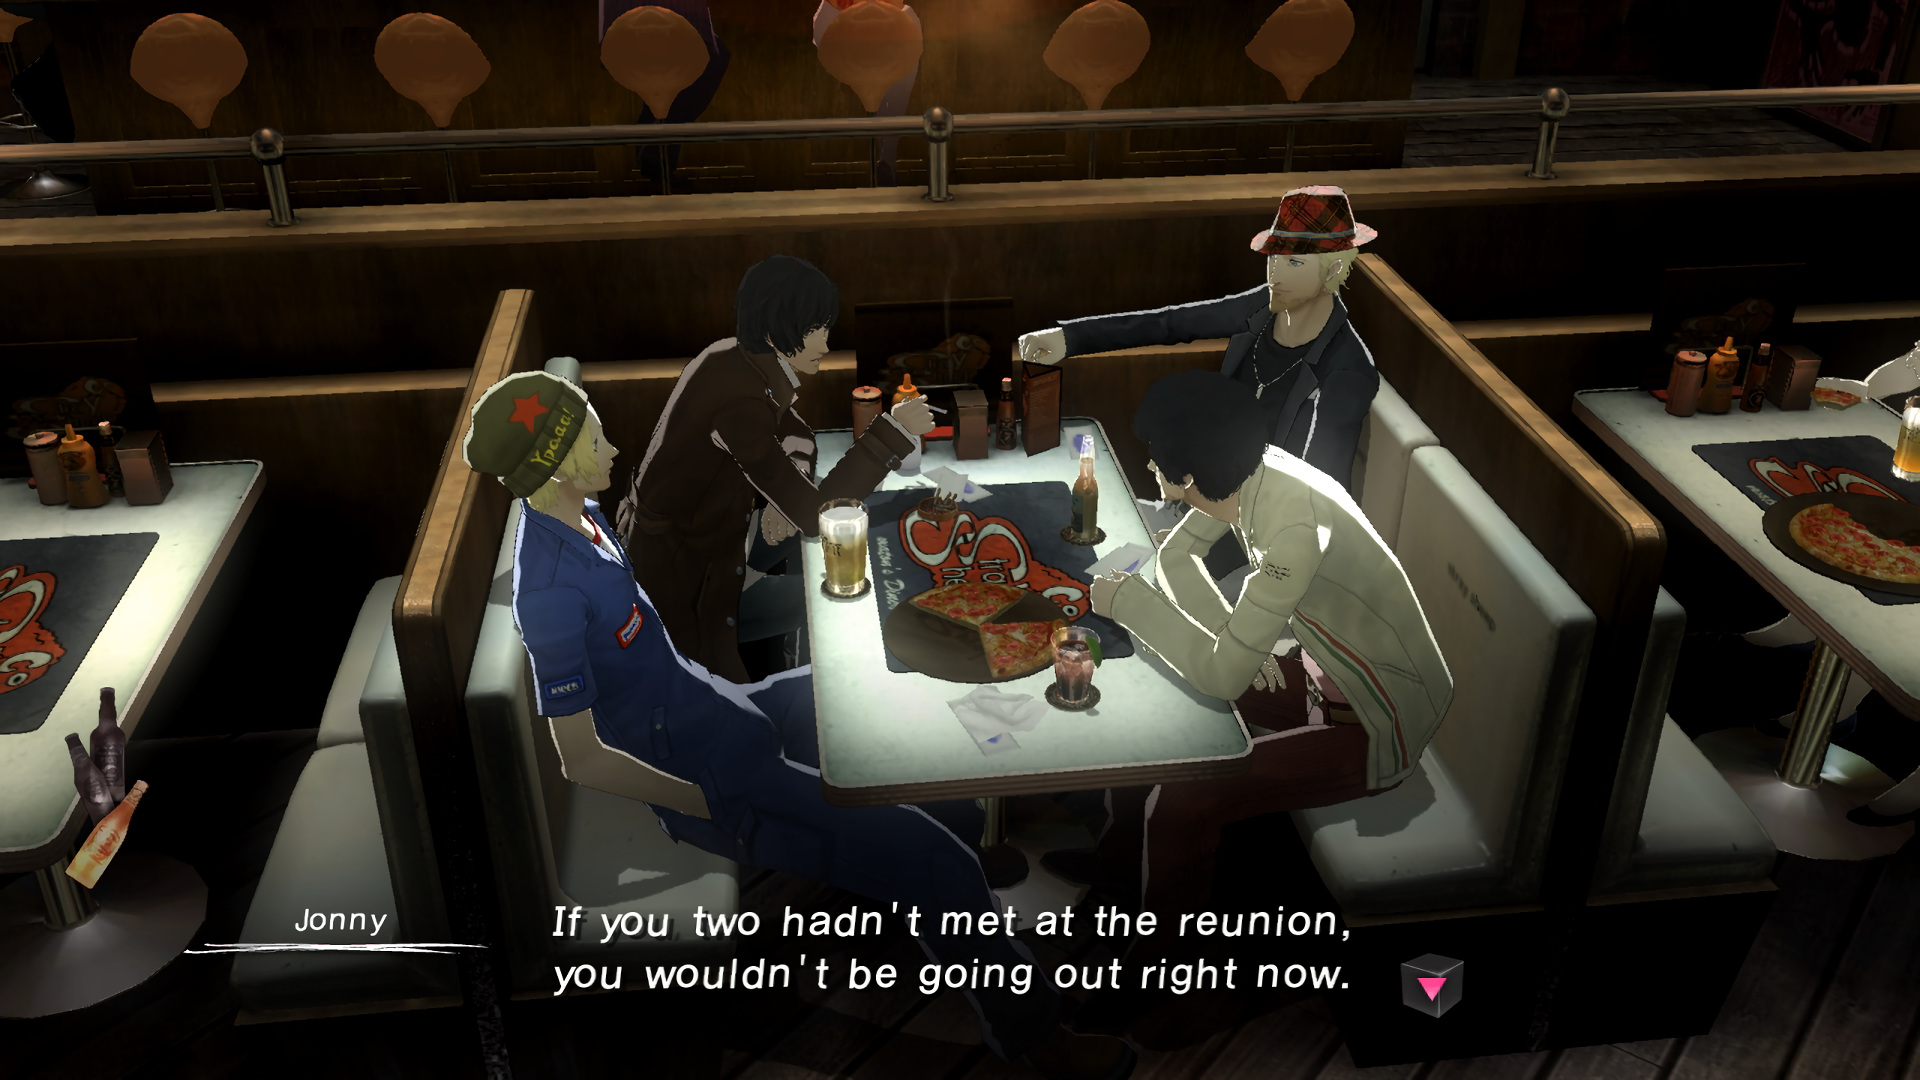
\includegraphics[width = 1\textwidth]{Imagenes/Sample_Trash_Char.png}
	\caption{Imagen ejemplo.}
	\label{fig:Trash_Char}
\end{figure}

El texto esperado de la figura \ref{fig:Trash_Char} es la siguiente:
\begin{verbatim}
	Jonny
	If you two hadn't met at the reunion,
	you wouldn't be going out right now.
\end{verbatim}
Y una posible salida de la OCR con la figura \ref{fig:Trash_Char} puede ser la siguiente:
\begin{verbatim}
T A W
Wml"lll"|||"lll“1]]“11‘“"1“l‘l]1"]]]"]]1"1V‘“"‘”V"”””””“WWHH\HH\HH
G
wiui:lfifl}m;,;r}l’“
Nul1l1lmu11111um111llumI11llumIIIIIIMMI1IllMmlllIIIUU1
Hunum;.x:flwww'M;‘dm‘w‘w‘w‘w‘uHfl“fl“flflmw e 4 ‘ w}\‘s.*"‘r Ll e e p
: L T Q1 A it e
- ' diiry el R ;4
o wm W el 5
i " :_.“;»"*‘ i i m?“ Q:‘]m}illl}jjw ! “hu‘11111111{}}“
T i 1‘11“1””“””““” HHHHHHH ‘HHU”“HH\HHHHH\HMH\H ‘ (TR
I e > h ¢ 4 ' i
= 4 o
T
- i e
§ ...
E ‘E | \ i
P S y:
,,|,- |
IR ill ‘
— ' A 000 Ir yo
\end{verbatim}

Donde de forma subjetiva no encontramos ningún trozo del texto que se corresponda o sea parecido al ground-truth.

Después de aplicar el preprocesamiento elegido en el apartado anterior obtenemos el siguiente resultado:

\begin{verbatim}
T A W
Wml"lll"|||"lll“1]]“11‘“"1“l‘l]1"]]]"]]1"1V‘“"‘”V"”””””“WWHH\H
dJonny If you two hadn't met at the reunion 
you wouldn't be going out right now
,,|,- |
IR ill ‘
— ' A 000 Ir yo
\end{verbatim}

En esta salida ya podemos reconocer que hay dos líneas que se corresponde con la salida que esperamos.
La frase que realmente importa es solamente las dos líneas de la salida.
\begin{verbatim}
Jonny If you two hadn't met at the reunion
you wouldn't be going out right now
\end{verbatim}
Esto es un problema importante que debemos solucionar ya que es imposible saber si un test es correcto o no con esta entrada.

En esta sección se propone una solución a este problema de caracteres ``basura'' usando el algoritmo de distancia \emph{levenshtein}.

La distancia de Levenshtein(también conocida como distancia de edición) según un articulo de \cite{LevDistance} se define como una métrica que mide el número mínimo de operaciones necesarias para transformar una cadena en otra, utilizando tres tipos de operaciones básicas:
\begin{itemize}
\item Inserciones: Agregar un carácter.
\item Eliminaciones: Eliminar un carácter.
\item Sustituciones: Reemplazar un carácter por otro.
\end{itemize}


Suponiendo que tenemos el texto esperado de la imagen,  utilizando esta métrica, podemos obtener la distancia levenshtein entre una línea del texto esperado y una línea del texto reconocido por la OCR. Con la distancia obtenida podemos calcular la similitud de las cadenas y aplicando un cierto umbral, podemos identificar aquellas líneas que más se asimila al texto esperado, obteniendo así las líneas deseadas y descartando aquellas que no cumpla un cierto umbral.

La fórmula general para calcular la similitud es:

$Simulitud = 1-\frac{d}{max(s1,s2)} $ 

Donde:

\textit{d} es la distancia levenshtein.

\textit{max(s1,s2)}	 es el máximo entre la longitud de la cadena \textit{s1} y cadena \textit{s2}

Uno de los resultados obtenidos aplicando la distancia levenshtein es la siguiente si aplicamos un umbral de similitud de 0.8 (tiene que ser 80\% de parecido):
\begin{itemize}
\item Texto real de OCR:
\begin{verbatim}
"
|
\ J
—
Agumon /
Still, a “smahrt fown” is cool! It really can
do anything! <
\end{verbatim}
\item Texto esperado:
\begin{verbatim}
Agumon
Still,a "smahrt fown" is cool! It really can
do anything!
\end{verbatim}

El algoritmo de limpieza sigue los siguientes pasos:

\begin{enumerate}
	\item Se compara la primera línea obtenida por el OCR con la primera línea del texto esperado.
	\item Se calcula la distancia de Levenshtein entre ambas cadenas.
	\item A partir de la distancia de Levenshtein y la longitud de las cadenas, se calcula el valor de similitud.
	\item Se verifica si la similitud supera el umbral previamente definido.
	\item Si la similitud es superior al umbral, se marca la línea como válida. En caso contrario, se continúa con la siguiente línea del texto esperado.
	\item Este proceso se repite hasta haber comparado la línea del OCR con todas las líneas del texto esperado. Si durante la iteración se encuentra una línea con una similitud mayor que la obtenida hasta el momento, se actualiza la línea marcada con esta nueva coincidencia.
	\item El mismo procedimiento se repite para la segunda línea del OCR y para el resto de líneas subsiguientes.
\end{enumerate}
Después de todo ese proceso obtenemos la cadena limpiada utilizando distancia levenshtein.
\item Tras aplicar este algoritmo, la cadena de OCR resultante será la siguiente:
\begin{verbatim}
Agumon /
Still "smahrt fown" is cool! It really can 
do anything! <
\end{verbatim}
\end{itemize}  
Aplicando el algoritmo a los resultados de todas las imágenes de cada categoría mencionadas en el apartado anterior después de aplicar preprocesamiento obtenemos estos nuevos resultados del CER medio de cada categoría:

\begin{table}[H]
\begin{tabular}{llllll}
Tipo        & Complejo & Simple & PixelArt & TxTBoc & TxtBoc2                      \\
OCR         & 2.57     & 0.29   & 2.01     & 1.01   & \cellcolor[HTML]{FFFFFF}1.49 \\
Levenshtein & 0.63     & 0.16   & 0.63     & 0.55   & 0.42                        
\end{tabular}
\end{table}
El resultado de OCR es el resultado que obtenemos con solamente aplicando el preprocesamiento del apartado anterior. Sobre esa salida, se aplica la distancia levenshtein para la eliminación de basura obteniendo los nuevos resultados. Podemos ver en los números que mejoran casi un 50\% en todas la categorías por lo que es una técnica viable para nuestra herramienta.
\section{Evaluación de los tests}
El objetivo de esta evaluación es asegurar de que los tests implementados sean correctos sin producir ningún falso positivo y falso negativo.
La metodología de la evaluación es utilizando test de unidad donde existirá una suite de test para casos positivos de cada test y casos negativos de cada test. 
\subsection{Test de placeholders}
Se define en este test un delimitador de placeholder indicado su cadena de apertura y su cadena de cierre. Se comprueba en los test de casos positivos que el texto no tenga ningún placeholder. Se comprueba en los test de casos negativos que reconozca el placeholder del texto en cualquier posición. P.ej se define la cadena de apertura de placeholder ``\%\_'' y la de cierre ``\_\%'' y se obtiene el resultado de la tabla \ref{table:tu_p} indicando positivo que pasa el test(no hay placeholder) y negativo que no pasa el test de placeholder(hay placeholder).
\begin{table}[H]
	\centering
	\begin{tabular}{ll}
	Texto & Resultado \\
	Sin placeholder & Positivo \\
	\%Sin placeholder\% & Positivo \\
	\%\_Placeholders\_\% & Negativo \\
	hola\%\_Placeholders\_\% & Negativo \\
	\end{tabular}
	\caption{Ejemplo de algunos test de unidad de placeholder}
	\label{table:tu_p}
\end{table}
\subsection{Test de solapamiento}
Para este test, se ha creado imágenes simples donde existen solapamiento de texto y otras en las cuales no hay. El suite test positivo verifica que no existen solapamiento por lo que pasa el test y el suite negativo verifica que existe solapamiento por lo que no lo pasa.
Las imágenes positivas y negativas tienen un aspecto similar a la figura \ref{fig:C} y la figura \ref{fig:F} .
\begin{figure}[H]
	\centering
	\begin{minipage}{0.45\textwidth}
		\centering
		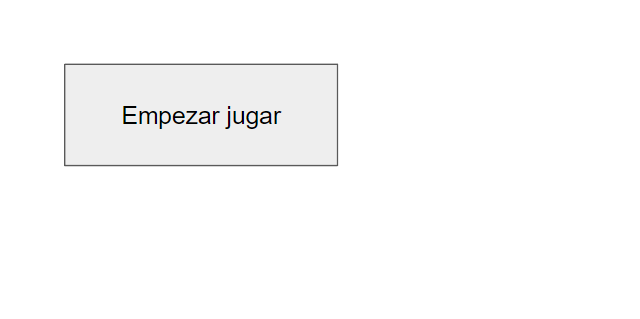
\includegraphics[width=\linewidth]{Imagenes/Eva/C.png}
		\caption{Ejemplo de imagen positivo en solapamiento.}
		\label{fig:C}
	\end{minipage}
	\hfill
	\begin{minipage}{0.45\textwidth}
		\centering
		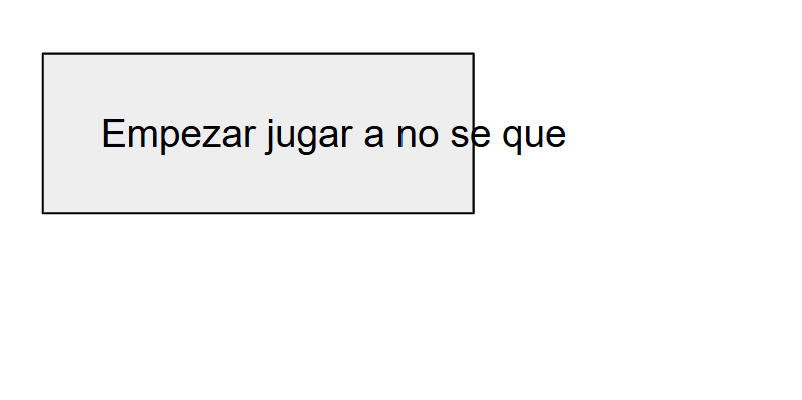
\includegraphics[width=\linewidth]{Imagenes/Eva/F.png}
		\caption{Ejemplo de imagen negativo en solapamiento.}
		\label{fig:F}
	\end{minipage}
\end{figure}
\subsection{Test de truncamiento}
En este test, para el suite de test positivos, se define la cadena del texto esperado y el texto reconocido de forma simétrica comprobando que pasa el test de truncamiento. En el suite de negativos, se define la cadena del texto esperado, y las cadenas del texto reconocido son subcadenas del texto esperado.P.ej :
\begin{itemize}
	\item Texto esperado: Empezar jugar
	\item Texto reconocido: Empezar jug
\end{itemize}
\subsection{Resultado del test de unidad}
Se ejecutan:
\begin{itemize}
	\item Placeholder: 8 casos positivos y 5 casos negativos.
	\item Solapamiento: 2 casos positivos y 2 casos negativos.
	\item Truncamiento: 2 casos positivos y 3 casos negativos.
\end{itemize}
Ejecutando el test de unidad obtenemos que se ha pasado todos los tests, tanto positivos como negativos por lo que podemos llegar a la conclusión de que la implementación de los tests son correctas.


\section{Evaluación de la herramienta}
\label{sec:Evaluación_herramienta}
En esta sección se hará una evaluación de la herramienta comprobando el funcionamiento completo incluyendo los dos modulos de OCR y tests.
El objetivo de esta evaluación es asegurar de que nuestra herramienta es preciso y exacto como ayuda de la parte de LQA.
La metodología de la evaluación es la siguiente:
\begin{enumerate}
	\item Se ha creado una batería de pruebas con 30 imágenes en total. Entre las 30 imágenes, existen \begin{itemize}
		\item 7 errores de solapamiento
		\item 5 errores de truncamiento
		\item 5 errores de placeholders
	\end{itemize}
	Las imágenes de prueba con errores de localización se ha hecho editando sobre imágenes de los juegos sobrescribiendo sobre el contenido original.
	\item Se ejecutará la herramienta propocionando información de estas imagenes y configuración.
	\item Se obtendrá los resultados de las imágenes.
	\item Se generará una matriz de confusión con los resultados obtenidos y esperados.
	\item Se obtendrá información de la matriz de confusión como precisión, falsos positivos y falsos negativos.
\end{enumerate}
En la matriz de confusión: 
\begin{itemize}
	\item Positivo representa que existe un error de localización.
	\item Negativo representa que no existe error de localización.
	\item El valor esperado es el resultado de la herramienta.
	\item El valor real es el valor que realmente es.
	\item Verdadero positivo(TP) indica que hay error y detecta error.
	\item Falso positivo(FP) indica que no hay error pero detecta error. 
	\item Verdadero negativo(TN) indica que no hay error y no detecta error.
	\item Falso negativo(FN) indica que hay error pero no detecta error. 
	\item Exactitud mide el porcentaje de predicciones correctas sobre el total de predicciones. Indica el porcentaje de acierto sobre si existe o no errores de localización en las imágenes.
	
	$Exactitud = \frac{TP + TN}{TP + TN + FP + FN}$
	
	\item Precisión mide el porcentaje de predicciones positivas correctas sobre el total de predicciones positivas. Indica el porcentaje de acierto de detección de errores de localización.
	
	$Precision = \frac{TP}{TP + FP}$
\end{itemize}
el aspecto de la matriz es similar a la tabla \ref{table:mt_ej}

\begin{table}[H]
	\centering
	\begin{tabular}{|c|c|c|c|}
		\hline
		& & Real &   \\
		\hline
		&          & Positivo & Negativo                   \\
		\hline
		Esperado & Positivo & TP& FP \\
		\hline
		& Negativo & 		  FN& TN                \\
		\hline
				&&&\\
		\hline
		&Exactitud&  & \\
		\hline
		&Precisión&  &\\
		\hline
	\end{tabular}
	\caption{Matriz de confusión ejemplo.}
	\label{table:mt_ej}
\end{table}
\begin{table}[H]
	\centering
	\begin{tabular}{|c|c|c|c|}
		\hline
		& & Real &   \\
		\hline
		&          & Positivo & Negativo                   \\
		\hline
		Esperado & Positivo & 14& 2 \\
		\hline
		& Negativo & 		  12& 2                 \\
 		\hline
 						&&&\\
 		\hline
 		&Exactitud& 53.33 & \\
 		\hline
 		&Precisión& 87.5 &\\
 		\hline
	\end{tabular}
	\caption{Matriz de confusión del resultado.}
	\label{table:mt_ori}
\end{table}

Como podemos observar en la tabla \ref{table:mt_ori} se producen 12 falsos negativos(se espera que detecte errores de localización pero la herramienta no lo detecta) y 2 falsos positivos(se esperaba que no exista ningún error de localización pero la herramienta los detecta como error). La cantidad de falsos positivos indica que la herramienta está detectando errores en imágenes donde no debería aparecer errores, esto es un problema para nuestra herramienta ya que nuestro fin es minimizar trabajo de un ser humano y este tipo de error aumenta el trabajo teniendo que evaluar las imágenes cuando en realidad no tiene ningún error. Y los falsos negativos indica que la herramienta no detecta ningún error en la imagen cuando en realidad existen errores lo que también es un problema porque la herramienta trata de reconocer errores para ser corregidos antes de la publicación del juego. Podemos observar que la precisión de la herramienta es alta(87.5\%) pero la exactitud es mediana(53.33\%) por lo cual la herramienta puede estar detectando errores de localización pero mucha de las veces falla en clasificar si una imagen tiene o no error de localización.

Para obtener más detalle de la evaluación, generaremos una matriz de confusión para cada tipo de test.

\begin{table}[H]
	\centering
	\begin{tabular}{|c|c|c|c|}
		\hline
		& & Real &   \\
		\hline
		&          & Positivo & Negativo                   \\
		\hline
		Esperado & Positivo & 3& 4 \\
		\hline
		& Negativo & 		  7& 16                 \\
		\hline
 						&&&\\
		\hline
		&Exactitud& 63.33 & \\
		\hline
		&Precisión& 42.86 &\\
		\hline
	\end{tabular}
	\caption{Matriz de confusión del resultado de solapamiento.}
	\label{table:mt_ori_sol}
\end{table}

\begin{table}[H]
	\centering
	\begin{tabular}{|c|c|c|c|}
		\hline
		& & Real &   \\
		\hline
		&          & Positivo & Negativo                   \\
		\hline
		Esperado & Positivo & 5& 0 \\
		\hline
		& Negativo & 		  20& 5                 \\
		\hline
		 						&&&\\
		\hline
		&Exactitud& 33.33 & \\
		\hline
		&Precisión& 100 &\\
		\hline
	\end{tabular}
	\caption{Matriz de confusión del resultado de truncamiento.}
\label{table:mt_ori_trun}
\end{table}
\begin{table}[H]
	\centering
	\begin{tabular}{|c|c|c|c|}
		\hline
		& & Real &   \\
		\hline
		&          & Positivo & Negativo                   \\
		\hline
		Esperado & Positivo & 0& 5 \\
		\hline
		& Negativo & 		  0& 25                \\
		\hline
		 						&&&\\
		\hline
		&Exactitud& 83.33 & \\
		\hline
		&Precisión& 0 &\\
		\hline
	\end{tabular}
	\caption{Matriz de confusión del resultado de placeholders.}
\label{table:mt_ori_place}
\end{table}
Mirando los resultados de cada test, podemos observar en la tabla \ref{table:mt_ori_sol}, se producen 11 errores(falso positivo + falso negativo) al detectar solapamiento lo cual ha conseguido acertar en 19 imágenes(63.33\% de exactitud) y que de los 7 errores que había, ha conseguido detectar 3(42.86\% de precisión). Sin embargo en las otras dos existen errores graves. En la tabla \ref{table:mt_ori_trun} podemos observar que se detectan 20 casos de falsos negativos que es un valor bastante alto lo que baja la exactitud a un 33.33\%. En la tabla \ref{table:mt_ori_place} observamos que se produce 25 casos de verdaderos negativos y 5 casos de falsos positivos, aunque parezca que tiene buenos resultados, recordamos que existe 5 errores de placeholders solamente, lo cual significa que no ha conseguido detectar ninguno de ellos(0\% de precisión). 
Lo que tienen en común estos últimos dos test es que usan el texto reconocido en la salida del OCR lo cual el problema puede encontrarse allí.

Observando el informe los resultados de salida, de las 30 imágenes de prueba, el porcentaje de similitud de 17 imágenes son menores del 50\% y entre ellas, 14 son 0\%, esto significa que no se esta reconociendo de forma correcta el texto de las imágenes produciendo todo ese error en los tests. Por tanto, aunque en la tabla \ref{table:mt_ori_trun} obtenga una precisión de 100\%, esto puede ser debido al mal reconocimiento de texto produciendo un error de truncamiento y que ``justamente'' en esas imágenes existen error de truncamiento.

Haciendo una investigación del problema, se detecta que el problema puede ser producido en el proceso de preprocesamiento, por lo cual mostramos por salida el resultado de la imagen después del preprocesamiento de la figura \ref{fig:Eva_2} (imagen original) obteniendo el resultado como se muestra en la figura \ref{fig:Eva_2P}.
\begin{figure}[H]
	\centering
	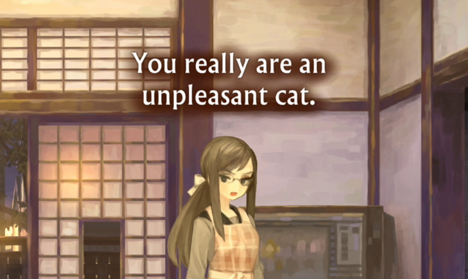
\includegraphics[width = 0.6\textwidth]{Imagenes/Evaluacion_OCR/2.png}
	\caption{Imagen ejemplo de prueba.}
	\label{fig:Eva_2}
\end{figure}
\begin{figure}[H]
	\centering
	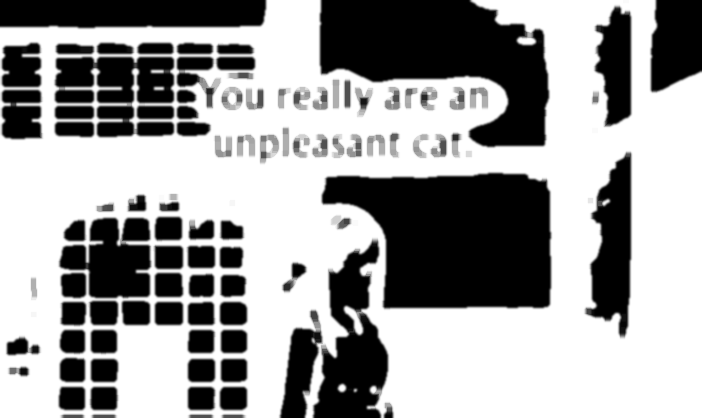
\includegraphics[width = 0.6\textwidth]{Imagenes/Evaluacion_OCR/2_prepro.png}
	\caption{Resultado de la imagen de prueba después de preprocesamiento.}
	\label{fig:Eva_2P}
\end{figure}

Podemos ver que la imagen preprocesada se ve borroso en la parte del texto incluso a ojo humano, por tanto es de lo esperado que el OCR no consiga reconocer el texto de la imagen.
Este problema es debido a que en la sección \ref{sec:Mejoras en el reconocimiento}, la evaluación del CER de los preprocesamientos se ha hecho sin tener en cuenta la distancia levenshtein que fue implementado y evaluado posteriormente del preprocesamiento. El bajo CER que se obtuvo es debido a que el OCR reconocía menos caracteres basura pero sin reconocer el texto. Puede darse el caso de que el OCR reconozca el texto pero con mucha basura, lo que  aumenta el CER, algo que se soluciona aplicando la distancia levenshtein.

Para intentar resolver este problema, evaluaremos la herramienta quitando los preprocesamientos que hagan que la imagen se vea más borroso que son:
\begin{itemize}
	\item Denoising
	\item Blurring
	\item Dilatar y erosionar.
\end{itemize}
\begin{figure}[H]
	\centering
	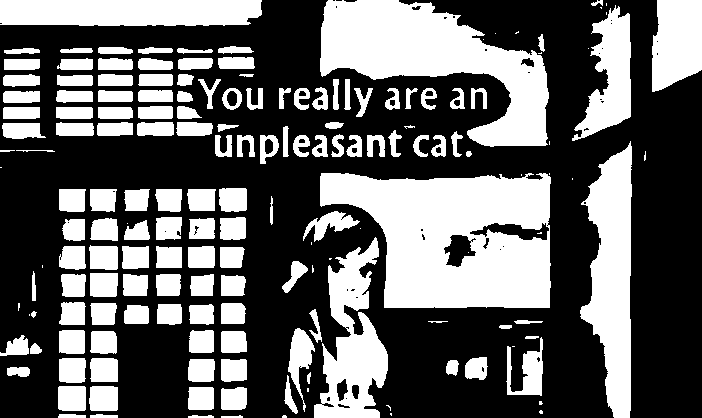
\includegraphics[width = 0.6\textwidth]{Imagenes/Evaluacion_OCR/2_p.png}
	\caption{Resultado de la imagen de prueba después del nuevo preprocesamiento.}
	\label{fig:Eva_2PP}
\end{figure}
Se obtiene la imagen que se muestra en la figura \ref{fig:Eva_2PP} y los siguientes nuevos resultados.
\begin{table}[H]
	\centering
	\begin{tabular}{|c|c|c|c|}
		\hline
		& & Real &   \\
		\hline
		&          & Positivo & Negativo                   \\
		\hline
		Esperado & Positivo & 15& 1 \\
		\hline
		& Negativo & 		  12& 2                \\
		\hline
		 						&&&\\
		\hline
		&Exactitud& 56.67 & \\
		\hline
		&Precisión& 93.75 &\\
		\hline
	\end{tabular}
	\caption{Matriz de confusión del resultado.}
\label{table:mt_pos}
\end{table}
\begin{table}[H]
	\centering
	\begin{tabular}{|c|c|c|c|}
		\hline
		& & Real &   \\
		\hline
		&          & Positivo & Negativo                   \\
		\hline
		Esperado & Positivo & 3& 4 \\
		\hline
		& Negativo & 		  7& 16                \\
		\hline
		 						&&&\\
		\hline
		&Exactitud& 63.33 & \\
		\hline
		&Precisión& 42.86 &\\
		\hline
	\end{tabular}
	\caption{Matriz de confusión del resultado de solapamiento.}
\label{table:mt_pos_sol}
\end{table}

\begin{table}[H]
	\centering
	\begin{tabular}{|c|c|c|c|}
		\hline
		& & Real &   \\
		\hline
		&          & Positivo & Negativo                   \\
		\hline
		Esperado & Positivo & 5& 0 \\
		\hline
		& Negativo & 		  20& 5                \\
		\hline
		 						&&&\\
		\hline
		&Exactitud& 33.33 & \\
		\hline
		&Precisión& 100 &\\
		\hline
	\end{tabular}
	\caption{Matriz de confusión del resultado de truncamiento.}
\label{table:mt_pos_trun}
\end{table}
\begin{table}[H]
	\centering
	\begin{tabular}{|c|c|c|c|}
		\hline
		& & Real &   \\
		\hline
		&          & Positivo & Negativo                   \\
		\hline
		Esperado & Positivo & 1& 4 \\
		\hline
		& Negativo & 		  0& 25                \\
		\hline
		 						&&&\\
		\hline
		&Exactitud& 86.67 & \\
		\hline
		&Precisión& 20 &\\
		\hline
	\end{tabular}
	\caption{Matriz de confusión del resultado de placeholders.}
\label{table:mt_pos_place}
\end{table}
Vemos que no ha mejorado mucho en la matriz de confusión, sin embargo si tenemos en cuenta el porcentaje de similitud como se observa en la tabla \ref{table:simi}, sí que se ha mejorado de forma genérica teniendo 15 imágenes por debajo del 50\% y entre ellas 9 imágenes de 0\%.

También observamos que en algunos casos ha empeorado, como puede ser la imagen 1 que tenía un 85\% y que ahora está a 0\%. 
\begin{table}[H]
	\centering
	\begin{tabular}{lll} 
		Imagen & Antes  & Después \\
		1  & 85.71 & 0      \\     
		2  & 0     & 0      \\  
		3  & 0     & 0      \\  
		4  & 0     & 100    \\  
		5  & 0     & 70.32  \\  
		6  & 0     & 70  \\ 
		7  & 0     & 81.63  \\  
		8  & 91    & 60.60  \\  
		9  & 86.66 & 86.66  \\  
		10 & 53.84 & 57.69  \\  
		11 & 75.67 & 59.35  \\  
		12 & 10.09 & 35.77  \\  
		13 & 54.92 & 54.92  \\  
		14 & 0     & 0      \\  
		15 & 0     & 0      \\  
		16 & 0     & 0      \\  
		17 & 0     & 0      \\  
		18 & 100   & 100    \\    
		19 & 0     & 0      \\     
		20 & 76.92 & 76.92  \\  
		21 & 54.05 & 51.35  \\  
		22 & 0     & 26.60  \\  
		23 & 0     & 35.77  \\  
		24 & 10    & 34.86  \\  
		25 & 69    & 47.88  \\  
		26 & 67    & 54.92  \\  
		27 & 0     & 0      \\  
		28 & 96    & 96     \\  
		29 & 30    & 30.30  \\  
		30 & 96.42 & 94.64  \\  
	\end{tabular}
		\caption{Comparación de porcentaje de similitud entre los dos preprocesamientos.}
	\label{table:simi}
\end{table}
Con esto podemos llegar a la conclusión de que es necesario diferente preprocesamiento dependiendo de las características de las imágenes.
Para ello, se intentará buscar el mejor preprocesamiento para cada imagen. Se ejecutará los siguientes tipos de preprocesamiento:
\begin{itemize}
	\item El preprocesado original de la sección \ref{sec:Mejoras en el reconocimiento}.
	\item El preprocesado mejorado de esta sección.
	\item Escala de grises y ajuste adaptativo de contraste.
	\item Escala de grises y simple thresholding.
	\item Escala de grises solamente.
\end{itemize}
Se aplican distintos métodos de preprocesado teniendo en cuenta que, en algunas imágenes, dicho preprocesado puede empeorar la calidad del reconocimiento, mientras que en otras resulta imprescindible para mejorar los resultados. Por ello, para cada imagen se evaluarán las diferentes opciones de preprocesado y se seleccionará aquella que obtenga el mayor porcentaje de similitud en el reconocimiento del texto.
Se obtiene los siguientes nuevos resultados:
\begin{table}[H]
	\centering
	\begin{tabular}{|c|c|c|c|}
		\hline
		& & Real &   \\
		\hline
		&          & Positivo & Negativo                   \\
		\hline
		Esperado & Positivo & 15& 1 \\
		\hline
		& Negativo & 		  10& 4                \\
		\hline
		&&&\\
		\hline
		&Exactitud& 63.33 & \\
		\hline
		&Precisión& 93.75 &\\
		\hline
	\end{tabular}
	\caption{Matriz de confusión del resultado.}
	\label{table:mt_n}
\end{table}
\begin{table}[H]
	\centering
	\begin{tabular}{|c|c|c|c|}
		\hline
		& & Real &   \\
		\hline
		&          & Positivo & Negativo                   \\
		\hline
		Esperado & Positivo & 4& 3 \\
		\hline
		& Negativo & 		  6& 17                \\
		\hline
		&&&\\
		\hline
		&Exactitud& 70 & \\
		\hline
		&Precisión& 57.14 &\\
		\hline
	\end{tabular}
	\caption{Matriz de confusión del resultado de solapamiento.}
	\label{table:mt_sol_n}
\end{table}

\begin{table}[H]
	\centering
	\begin{tabular}{|c|c|c|c|}
		\hline
		& & Real &   \\
		\hline
		&          & Positivo & Negativo                   \\
		\hline
		Esperado & Positivo & 5& 0 \\
		\hline
		& Negativo & 		  17& 8                \\
		\hline
		&&&\\
		\hline
		&Exactitud& 39.39 & \\
		\hline
		&Precisión& 62.5 &\\
		\hline
	\end{tabular}
	\caption{Matriz de confusión del resultado de truncamiento.}
	\label{table:mt_trun_n}
\end{table}
\begin{table}[H]
	\centering
	\begin{tabular}{|c|c|c|c|}
		\hline
		& & Real &   \\
		\hline
		&          & Positivo & Negativo                   \\
		\hline
		Esperado & Positivo & 1& 4 \\
		\hline
		& Negativo & 		  0& 25                \\
		\hline
		&&&\\
		\hline
		&Exactitud& 86.67 & \\
		\hline
		&Precisión& 20 &\\
		\hline
	\end{tabular}
	\caption{Matriz de confusión del resultado de placeholders.}
	\label{table:mt_place_n}
\end{table}
\begin{table}[H]
	\centering
	\begin{tabular}{lll} 
		Imagen & Antes  & Mejor de cada imagen. \\
		1  & 85.71 & 86      \\     
		2  & 0     & 70      \\  
		3  & 0     & 67      \\  
		4  & 0     & 100    \\  
		5  & 0     & 91  \\  
		6  & 0     & 70  \\ 
		7  & 0     & 89  \\  
		8  & 91    & 91  \\  
		9  & 86.66 & 86.66  \\  
		10 & 53.84 & 65  \\  
		11 & 75.67 & 75.67 \\  
		12 & 10.09 & 38  \\  
		13 & 54.92 & 83  \\  
		14 & 0     & 8      \\  
		15 & 0     & 73      \\  
		16 & 0     & 88      \\  
		17 & 0     & 76      \\  
		18 & 100   & 100    \\    
		19 & 0     & 65     \\     
		20 & 76.92 & 76.92  \\  
		21 & 54.05 & 70  \\  
		22 & 0     & 29  \\  
		23 & 0     & 38  \\  
		24 & 10    & 34.86  \\  
		25 & 69    & 76  \\  
		26 & 67    & 63  \\  
		27 & 0     & 45      \\  
		28 & 96    & 96     \\  
		29 & 30    & 79  \\  
		30 & 96.42 & 96.42  \\  
	\end{tabular}
	\caption{Comparación de porcentaje de similitud entre el preprocesado original y los mejores de cada imagen.}
	\label{table:simi_n}
\end{table}
Como podemos observar en las tablas \ref{table:mt_n}, \ref{table:mt_sol_n} y \ref{table:mt_trun_n}, se vuelve a mejorar un poco los resultados en cuanto la exactitud. El porcentaje de similitud en este caso ya no hay ningún valor a 0\% y solamente hay 6 imágenes con valores inferiores al 50\% como podemos ver en la tabla \ref{table:simi_n}. Este proceso de preprocesamiento específico para cada imagen no es trivial por lo que es necesario en un futuro obtener características de la imágenes y aplicar determinadas técnicas de preprocesamiento según las características.

Como se puede observar en las Tablas \ref{table:mt_n}, \ref{table:mt_sol_n} y \ref{table:mt_trun_n}, se aprecia una ligera mejora en los resultados de exactitud. En cuanto al porcentaje de similitud, ya no se presentan valores del 0\%, y únicamente seis imágenes registran valores inferiores al 50\%, como se detalla en la Tabla \ref{table:simi_n}. Este resultado indica que el uso de un preprocesamiento específico por imagen contribuye a mejorar el rendimiento del sistema. Sin embargo, este proceso no es trivial, por lo que en trabajos futuros sería recomendable extraer características relevantes de cada imagen y aplicar técnicas de preprocesamiento adaptadas a dichas características.

En conclusión, la precisión y exactitud de la herramienta se sitúan en un nivel intermedio y son claramente mejorables. Una de las principales limitaciones es que el OCR no logra reconocer el texto de forma completamente precisa, lo que sugiere que es necesario optimizar el preprocesamiento para mejorar el rendimiento del reconocimiento. Una posible línea de mejora sería el entrenamiento del modelo OCR con fuentes específicas del videojuego, ya que hasta ahora se ha utilizado únicamente el modelo por defecto de Tesseract.

\section{Conclusión}
En este capítulo se ha llevado a cabo la evaluación del módulo de OCR, del módulo de tests y, finalmente, de la herramienta en su conjunto. En la evaluación del módulo de OCR, Tesseract ha demostrado ser la opción más adecuada para el caso de uso planteado. Con el fin de mejorar el reconocimiento de texto, se han aplicado técnicas como el preprocesamiento de imágenes, que facilita la detección de texto, y el uso de la distancia de Levenshtein para medir la similitud entre cadenas, lo cual permite filtrar caracteres irrelevantes o erróneos.

Para evaluar el módulo de tests se ha desarrollado una prueba unitaria específica, cuyos resultados han sido satisfactorios, demostrando el correcto funcionamiento del sistema de validación.

En cuanto a la evaluación global de la herramienta, los resultados obtenidos reflejan un rendimiento aceptable pero claramente mejorable. La principal limitación detectada radica en el reconocimiento textual por parte del OCR. Para mitigar este problema, se propone como línea de mejora futura la adaptación del preprocesamiento en función de las características de cada imagen, así como el entrenamiento de un modelo OCR específico para la fuente utilizada en el videojuego, en lugar de depender exclusivamente del modelo por defecto.
\chapter{Conclusiones y Trabajo Futuro}
\label{cap:conclusiones}

Debido a la gran evolución en la industria de los videojuegos, surge la necesidad de adaptar un videojuego a otro idioma/región diferente del que fue creado. Para ello, se siguen los procesos de internacionalización y localización, donde la internacionalización es la realización de soporte para diferentes idiomas y la localización es el proceso la cual se traducen y se adaptan los textos, gráficos, etc.

Para asegurar de que el videojuego está preparado para ser publicado en otras regiones, entra el \textit{Localization Quality Assurance} (o LQA) para asegurar de que no exista ningún error de localización.

Para facilitar el trabajo de LQA, se ha diseñado una herramienta donde el usuario proporciona unas imágenes del juego y una configuración, la herramienta detecte si existe algún error de localización. Esta herramienta constará de dos partes, modulo de OCR y modulo de tests.

Para el modulo de OCR, se evalua diferentes librerías de OCR y para nuestra herramienta, utilizaremos Tesseract. Para mejorar los resultados de reconocimiento, se aplica técnicas como preprocesamiento de imágenes para mejor identificación de texto en imágenes y técnicas como la distancia levenshtein para eliminar caracteres basuras reconocidas por el OCR.

Para el modulo de tests, que diseña y se implementa tests que puedan detectar errores de localización, para nuestro caso, se ha hecho el test de solapamiento de texto, truncamiento de texto y detección de placeholders.

La herramienta generará un archivos con los resultados que será luego interpretado generando así un informe.

Los resultados de la evaluación de la herramienta han sido aceptables, aunque claramente mejorables. La principal limitación observada reside en el reconocimiento de texto por parte del OCR, especialmente en imágenes complejas como las que se generan en un entorno de videojuego.

Para mejorar la herramienta se propone los siguiente trabajos futuros:

\begin{enumerate}
	\item Clasificación de imágenes para detectar el preprocesamiento necesario según las características de las imágenes.
	\item Árbol de decisión que configure un determinado preprocesamiento según las características de las imágenes.
	\item Entreno del modelo con la fuente específica.
	\item Integración de otras librerías de OCR como opción al usuario.
	\item Implementación de test que solucione otros problemas de localización.
	\item Detección de layout en las imágenes para reconocer las zonas de texto y hacer un recorte para eliminar zonas sin texto y mejorar el reconocimiento.
	\item Herramienta que recopile dato de pantalla de videojuego y generar los assets necesarios para la herramienta de detección de errores de localización.
\end{enumerate}


%%%%%%%%%%%%%%%%%%%%%%%%%%%%%%%%%%%%%%%%%%%%%%%%%%%%%%%%%%%%%%%%%%%%%%%%%%%
% Si el TFG se escribe en inglés, comentar las siguientes líneas 
% porque no es necesario incluir nuevamente las Conclusiones en inglés
\begin{otherlanguage}{english}
\chapter*{Introduction}
\label{cap:introduction}
\addcontentsline{toc}{chapter}{Introduction}

Introduction to the subject area. This chapter contains the translation of Chapter \ref{cap:introduccion}.

Nowadays, due to the large number of video game users in different regions, there arises a need to adapt video games to countries or regions different from where they were originally developed. For this purpose, there is a series of steps or strategies that can be followed. In this work, I will design a tool to assist in this process.

\section{Motivation}
Over the years, video games have become one of the largest entertainment industries in the world. According to a report by \cite{NZIngreso2024}, in 2024 the global video game market reached an estimated revenue of 187.7 billion dollars, as shown in Figure \ref{fig:NewZooRevenues_E}. The same report shows the growth in the number of players (Figure \ref{fig:NewzooPlayers_E}), from 3.14 billion in 2022 to 3.422 billion in 2024, with a prediction of 3.759 billion by 2027.

\begin{figure}[H]
	\centering
	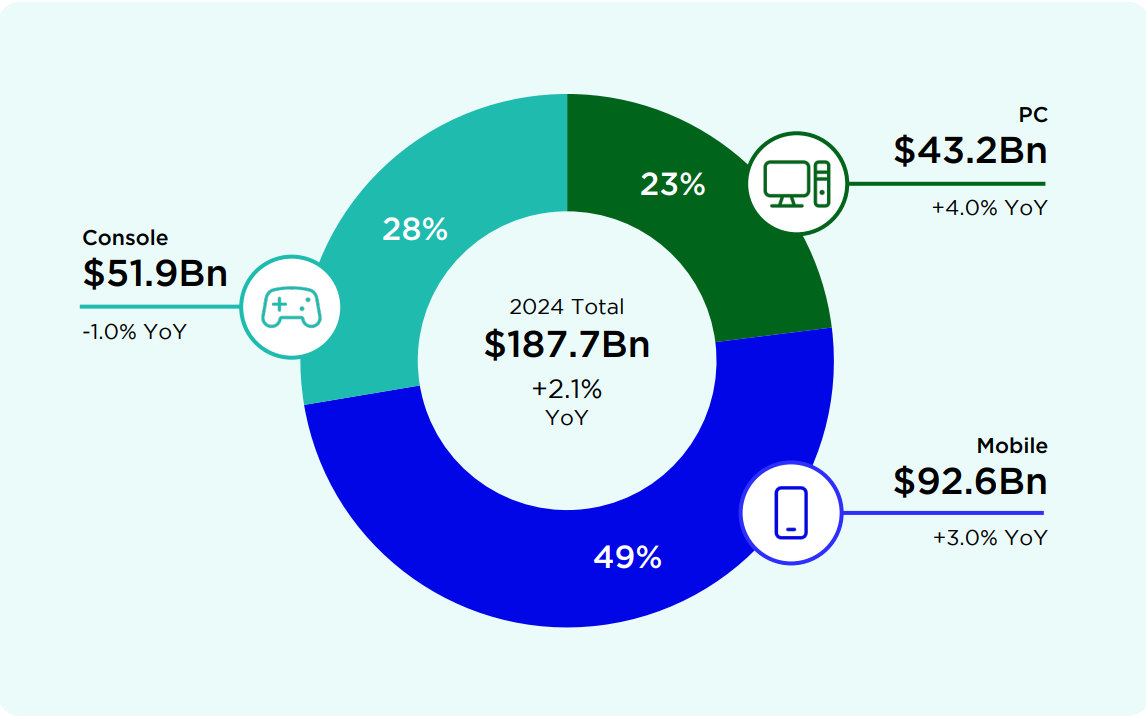
\includegraphics[width = 0.5\textwidth]{Imagenes/Newzoo_2024_Revenues.png}
	\caption{Estimated revenue in the video game industry in 2024. Newzoo}
	\label{fig:NewZooRevenues_E}
\end{figure}

\begin{figure}[H]
	\centering
	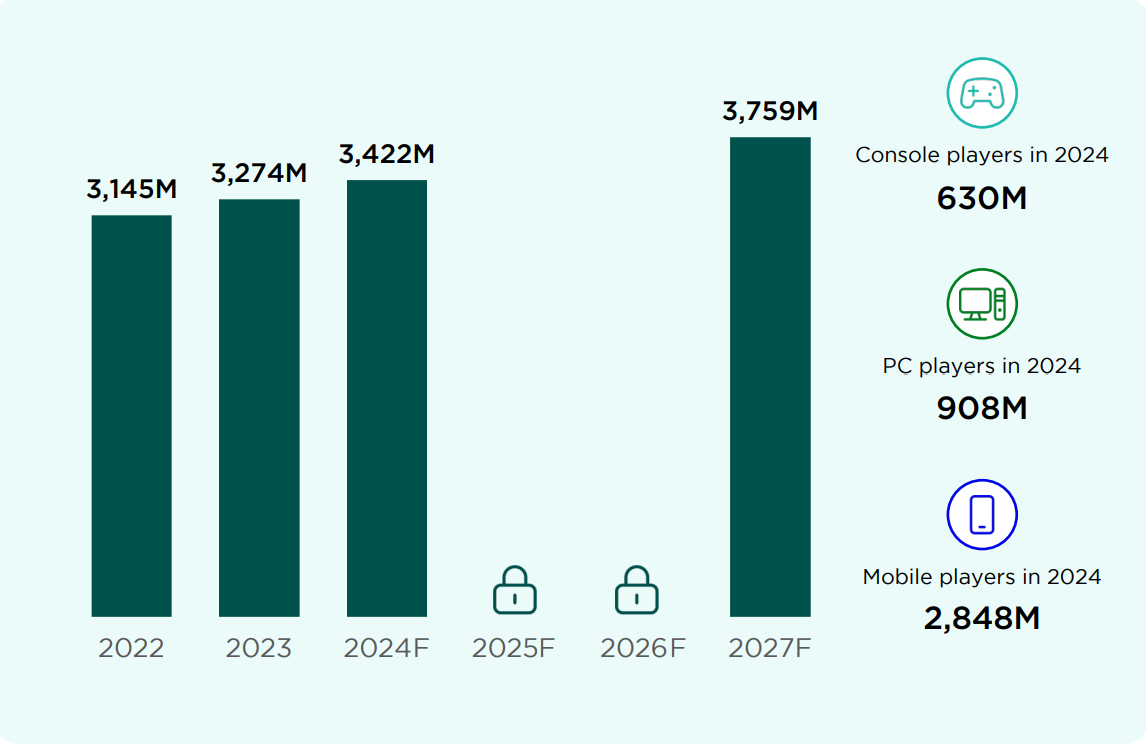
\includegraphics[width = 0.5\textwidth]{Imagenes/Newzoo_Players.png}
	\caption{Global players 2022–2024 and projection for 2027. Newzoo}
	\label{fig:NewzooPlayers_E}
\end{figure}

Additionally, the same report mentions the percentage of players by region, with the Asia-Pacific region representing more than half (53\%) of global players, as shown in Figure \ref{fig:NewzooPlayersReg_E}.  
Given this growth and these figures, there is a need to adapt video games to different languages and cultures through the processes of internationalization ({\textit{I18N}}) and localization ({\textit{L10N}}), in order to be published in various regions and countries.

\begin{figure}[H]
	\centering
	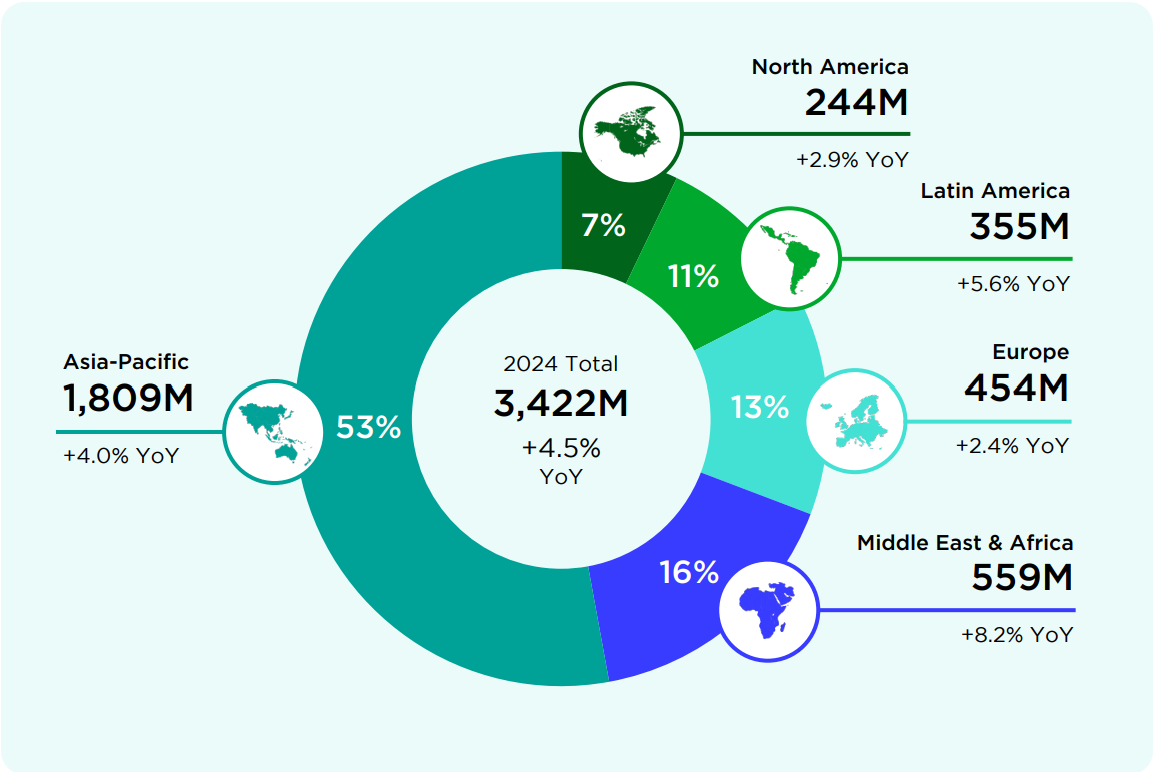
\includegraphics[width = 0.5\textwidth]{Imagenes/Newzoo_Players_Region.png}
	\caption{Percentage of players by region. Newzoo}
	\label{fig:NewzooPlayersReg_E}
\end{figure}

Internationalization is the process by which a video game is prepared from its early development stages to support different cultures and languages, so that no major modifications to the code are needed later.  
On the other hand, localization is the process of translating and adapting the texts, graphics, and resources of a video game to the various cultures in which it will be released.

During both of these processes, various types of errors may occur (such as translation or display errors). This is where \textit{Localization Quality Assurance} (LQA) comes into play. This process involves reviewing and testing different parts of the game to ensure that none of these errors occur and that the final product is appropriate for the target culture and audience.

Until now, this process has been carried out manually, where testers meticulously check each piece of text and how it is displayed within the game, which requires a significant amount of time and resources. While there are tools to automatically check the correctness of translations and texts, the same cannot be said for verifying how texts are displayed within the context of the game.

Based on the points discussed above, our motivation for this work is to automate testing of internationalization and localization processes in order to save time and resources, which can then be redirected to other more critical areas.  
To achieve this, we will use computer vision techniques and \textit{Optical Character Recognition} (OCR) so that, given a screenshot of a video game, we can extract the text and perform various checks and tests on it.

\section{Objectives}
The main objective of this project is the design and implementation of a tool to assist in the automation of localization QA.  
To achieve this main goal, the following secondary objectives are proposed:

\begin{enumerate}
	\item Research the LQA process and the tools used, as well as the most common errors in internationalization and localization.
	\item Investigate OCR technologies and how to use them, in order to choose one that fits our requirements by conducting tests and comparisons.
	\item Design a series of OCR-based automated tests to detect common linguistic errors.
	\item Deploy the tool using a Docker image so that it can be run on any machine.
	\item Integrate the OCR to use its output as input for the tests, and improve the OCR's accuracy as much as possible.
	\item Evaluate our tool to ensure it produces an acceptable accuracy rate.
\end{enumerate}

\section{Work Plan}
To achieve our objectives, we will follow the steps below:

\begin{enumerate}
	\item Research and understand the processes of internationalization, localization, and LQA, as well as the most common linguistic errors that occur during video game development (Chapter \ref{cap:estadoDeLaCuestion}).
	\item Select the most common localization errors that are related to character or positioning issues and that can be detected using OCR (Chapter \ref{cap:descripcionTrabajo}).
	\item Develop a series of tests capable of detecting specific localization errors using OCR-generated data as input (Chapter \ref{cap:implementacion}).
	\item Investigate different OCRs, understand how they work, how to use them to detect text in images, and how to train a model knowing the language and font used (Section \ref{sec:Seleccion de libreria de OCR}).
	\item Evaluate the selected OCRs based on performance and accuracy. Explore methods to increase accuracy (Chapter \ref{cap:evaluacion}).
	\item Perform separate evaluations of each module (OCR and testing) (Chapter \ref{cap:evaluacion}).
	\item Integrate both modules and conduct a comprehensive evaluation of the entire tool (Chapter \ref{cap:evaluacion}).
	\item Generate output that is easily interpretable by humans (Section \ref{sec:Generación informe}).
\end{enumerate}









\chapter*{Conclusions and Future Work}
\label{cap:conclusions}
\addcontentsline{toc}{chapter}{Conclusions and Future Work}

Conclusions and future lines of work. This chapter contains the translation of Chapter \ref{cap:conclusiones}.

In conclusion, due to the significant evolution of the video game industry, there arises a need to adapt a video game to different language or region from the one in which it was originally developed. For this purpose, the processes of internationalization and localization are followed, where internationalization refers to providing support for different languages, and localization is the process in which the texts, graphics and game assets are translated and adapted.

To ensure that the game is ready to be published in other regions, \textit{Localization Quality Assurance} (LQA) is carried out to verify that there are no localization errors.

To assist the LQA process, a tool is designed where the user provides game screenshots and a configuration file, and the tool detects whether any localization errors exist. This tool consists of two parts: an OCR module and a test module.

For the OCR module, several OCR libraries are evaluated, and for our tool, Tesseract is used. To improve text recognition results, techniques such as image preprocessing are applied to better identify text in images, as well as methods like Levenshtein distance to remove noisy characters recognized by the OCR.

For the test module, tests are designed and implemented to detect localization errors. In our case, the implemented tests include text overlap, text truncation, and placeholder detection.

The tool will generate a result file that will later be interpreted to create a report.

The evaluation results of the tool were not very promising. There is a problem in recognizing text in complex images such as those from video games, which leads to poor test results due to the quality of the input data.

To improve the tool, the following future work is proposed:

\begin{enumerate}
	\item Image classification to detect the necessary preprocessing according to the characteristics of the images.
	\item Decision tree to configure a specific preprocessing pipeline based on image features.
	\item Integration of other OCR libraries as options for the user.
	\item Implementation of new tests to address other localization issues.
	\item Layout detection in images to recognize text regions and crop out irrelevant areas to improve recognition.
	\item A tool that captures video game screen data and generates the necessary assets for the localization error detection tool.
\end{enumerate}

\end{otherlanguage}
%%%%%%%%%%%%%%%%%%%%%%%%%%%%%%%%%%%%%%%%%%%%%%%%%%%%%%%%%%%%%%%%%%%%%%%%%%%

%\chapter*{Contribuciones Personales}
\label{cap:contribucionesPersonales}
\addcontentsline{toc}{chapter}{Contribuciones Personales}

En caso de trabajos no unipersonales, cada participante indicará en la memoria su contribución al proyecto con una extensión de al menos dos páginas por cada uno de los participantes.

En caso de trabajo unipersonal, elimina esta página en el fichero \texttt{TFGTeXiS.tex} (comenta o borra la línea \verb|\chapter*{Contribuciones Personales}
\label{cap:contribucionesPersonales}
\addcontentsline{toc}{chapter}{Contribuciones Personales}

En caso de trabajos no unipersonales, cada participante indicará en la memoria su contribución al proyecto con una extensión de al menos dos páginas por cada uno de los participantes.

En caso de trabajo unipersonal, elimina esta página en el fichero \texttt{TFGTeXiS.tex} (comenta o borra la línea \verb|\chapter*{Contribuciones Personales}
\label{cap:contribucionesPersonales}
\addcontentsline{toc}{chapter}{Contribuciones Personales}

En caso de trabajos no unipersonales, cada participante indicará en la memoria su contribución al proyecto con una extensión de al menos dos páginas por cada uno de los participantes.

En caso de trabajo unipersonal, elimina esta página en el fichero \texttt{TFGTeXiS.tex} (comenta o borra la línea \verb|\include{Capitulos/ContribucionesPersonales}|).

\section*{Estudiante 1}
Al menos dos páginas con las contribuciones del estudiante 1.

\section*{Estudiante 2}
Al menos dos páginas con las contribuciones del estudiante 2. En caso de que haya más estudiantes, copia y pega una de estas secciones.

|).

\section*{Estudiante 1}
Al menos dos páginas con las contribuciones del estudiante 1.

\section*{Estudiante 2}
Al menos dos páginas con las contribuciones del estudiante 2. En caso de que haya más estudiantes, copia y pega una de estas secciones.

|).

\section*{Estudiante 1}
Al menos dos páginas con las contribuciones del estudiante 1.

\section*{Estudiante 2}
Al menos dos páginas con las contribuciones del estudiante 2. En caso de que haya más estudiantes, copia y pega una de estas secciones.



%
% Bibliografía
%
% Si el TFM se escribe en inglés, editar TeXiS/TeXiS_bib para cambiar el
% estilo de las referencias
%---------------------------------------------------------------------
%
%                      configBibliografia.tex
%
%---------------------------------------------------------------------
%
% bibliografia.tex
% Copyright 2009 Marco Antonio Gomez-Martin, Pedro Pablo Gomez-Martin
%
% This file belongs to the TeXiS manual, a LaTeX template for writting
% Thesis and other documents. The complete last TeXiS package can
% be obtained from http://gaia.fdi.ucm.es/projects/texis/
%
% Although the TeXiS template itself is distributed under the 
% conditions of the LaTeX Project Public License
% (http://www.latex-project.org/lppl.txt), the manual content
% uses the CC-BY-SA license that stays that you are free:
%
%    - to share & to copy, distribute and transmit the work
%    - to remix and to adapt the work
%
% under the following conditions:
%
%    - Attribution: you must attribute the work in the manner
%      specified by the author or licensor (but not in any way that
%      suggests that they endorse you or your use of the work).
%    - Share Alike: if you alter, transform, or build upon this
%      work, you may distribute the resulting work only under the
%      same, similar or a compatible license.
%
% The complete license is available in
% http://creativecommons.org/licenses/by-sa/3.0/legalcode
%
%---------------------------------------------------------------------
%
% Fichero  que  configura  los  parámetros  de  la  generación  de  la
% bibliografía.  Existen dos  parámetros configurables:  los ficheros
% .bib que se utilizan y la frase célebre que aparece justo antes de la
% primera referencia.
%
%---------------------------------------------------------------------


%%%%%%%%%%%%%%%%%%%%%%%%%%%%%%%%%%%%%%%%%%%%%%%%%%%%%%%%%%%%%%%%%%%%%%
% Definición de los ficheros .bib utilizados:
% \setBibFiles{<lista ficheros sin extension, separados por comas>}
% Nota:
% Es IMPORTANTE que los ficheros estén en la misma línea que
% el comando \setBibFiles. Si se desea utilizar varias líneas,
% terminarlas con una apertura de comentario.
%%%%%%%%%%%%%%%%%%%%%%%%%%%%%%%%%%%%%%%%%%%%%%%%%%%%%%%%%%%%%%%%%%%%%%
\setBibFiles{%
biblio%
}

%%%%%%%%%%%%%%%%%%%%%%%%%%%%%%%%%%%%%%%%%%%%%%%%%%%%%%%%%%%%%%%%%%%%%%
% Definición de la frase célebre para el capítulo de la
% bibliografía. Dentro normalmente se querrá hacer uso del entorno
% \begin{FraseCelebre}, que contendrá a su vez otros dos entornos,
% un \begin{Frase} y un \begin{Fuente}.
%
% Nota:
% Si no se quiere cita, se puede eliminar su definición (en la
% macro setCitaBibliografia{} ).
%%%%%%%%%%%%%%%%%%%%%%%%%%%%%%%%%%%%%%%%%%%%%%%%%%%%%%%%%%%%%%%%%%%%%%
\setCitaBibliografia{
\begin{FraseCelebre}
\begin{Frase}
  Y así, del mucho leer y del poco dormir, se le secó el celebro de
  manera que vino a perder el juicio.\\ 
  \textcolor{red}{(modificar en Cascaras$\backslash$bibliografia.tex)}
\end{Frase}
\begin{Fuente}
  Miguel de Cervantes Saavedra
\end{Fuente}
\end{FraseCelebre}
}

%%
%% Creamos la bibliografia
%%
\makeBib

% Variable local para emacs, para  que encuentre el fichero maestro de
% compilación y funcionen mejor algunas teclas rápidas de AucTeX

%%%
%%% Local Variables:
%%% mode: latex
%%% TeX-master: "../Tesis.tex"
%%% End:



% Apéndices
%\appendix
%\chapter{Título del Apéndice A}
\label{Appendix:Key1}

Los apéndices son secciones al final del documento en las que se agrega texto con el objetivo de ampliar los contenidos del documento principal.
%\chapter{Título del Apéndice B}
\label{Appendix:Key2}

Se pueden añadir los apéndices que se consideren oportunos.
%\include{Apendices/appendixC}
%\include{...}
%\include{...}
%\include{...}
\backmatter



%
% Índice de palabras
%

% Sólo  la   generamos  si  está   declarada  \generaindice.  Consulta
% TeXiS.sty para más información.

% En realidad, el soporte para la generación de índices de palabras
% en TeXiS no está documentada en el manual, porque no ha sido usada
% "en producción". Por tanto, el fichero que genera el índice
% *no* se incluye aquí (está comentado). Consulta la documentación
% en TeXiS_pream.tex para más información.
\ifx\generaindice\undefined
\else
%%---------------------------------------------------------------------
%
%                        TeXiS_indice.tex
%
%---------------------------------------------------------------------
%
% TeXiS_indice.tex
% Copyright 2009 Marco Antonio Gomez-Martin, Pedro Pablo Gomez-Martin
%
% This file belongs to TeXiS, a LaTeX template for writting
% Thesis and other documents. The complete last TeXiS package can
% be obtained from http://gaia.fdi.ucm.es/projects/texis/
%
% This work may be distributed and/or modified under the
% conditions of the LaTeX Project Public License, either version 1.3
% of this license or (at your option) any later version.
% The latest version of this license is in
%   http://www.latex-project.org/lppl.txt
% and version 1.3 or later is part of all distributions of LaTeX
% version 2005/12/01 or later.
%
% This work has the LPPL maintenance status `maintained'.
% 
% The Current Maintainers of this work are Marco Antonio Gomez-Martin
% and Pedro Pablo Gomez-Martin
%
%---------------------------------------------------------------------
%
% Contiene  los  comandos  para  generar  el índice  de  palabras  del
% documento.
%
%---------------------------------------------------------------------
%
% NOTA IMPORTANTE: el  soporte en TeXiS para el  índice de palabras es
% embrionario, y  de hecho  ni siquiera se  describe en el  manual. Se
% proporciona  una infraestructura  básica (sin  terminar)  para ello,
% pero  no ha  sido usada  "en producción".  De hecho,  a pesar  de la
% existencia de  este fichero, *no* se incluye  en Tesis.tex. Consulta
% la documentación en TeXiS_pream.tex para más información.
%
%---------------------------------------------------------------------


% Si se  va a generar  la tabla de  contenidos (el índice  habitual) y
% también vamos a  generar el índice de palabras  (ambas decisiones se
% toman en  función de  la definición  o no de  un par  de constantes,
% puedes consultar modo.tex para más información), entonces metemos en
% la tabla de contenidos una  entrada para marcar la página donde está
% el índice de palabras.

\ifx\generatoc\undefined
\else
   \addcontentsline{toc}{chapter}{\indexname}
\fi


% Generamos el índice
\printindex

% Variable local para emacs, para  que encuentre el fichero maestro de
% compilación y funcionen mejor algunas teclas rápidas de AucTeX

%%%
%%% Local Variables:
%%% mode: latex
%%% TeX-master: "./tesis.tex"
%%% End:

\fi

%
% Lista de acrónimos
%

% Sólo  lo  generamos  si  está declarada  \generaacronimos.  Consulta
% TeXiS.sty para más información.


\ifx\generaacronimos\undefined
\else
%---------------------------------------------------------------------
%
%                        TeXiS_acron.tex
%
%---------------------------------------------------------------------
%
% TeXiS_acron.tex
% Copyright 2009 Marco Antonio Gomez-Martin, Pedro Pablo Gomez-Martin
%
% This file belongs to TeXiS, a LaTeX template for writting
% Thesis and other documents. The complete last TeXiS package can
% be obtained from http://gaia.fdi.ucm.es/projects/texis/
%
% This work may be distributed and/or modified under the
% conditions of the LaTeX Project Public License, either version 1.3
% of this license or (at your option) any later version.
% The latest version of this license is in
%   http://www.latex-project.org/lppl.txt
% and version 1.3 or later is part of all distributions of LaTeX
% version 2005/12/01 or later.
%
% This work has the LPPL maintenance status `maintained'.
% 
% The Current Maintainers of this work are Marco Antonio Gomez-Martin
% and Pedro Pablo Gomez-Martin
%
%---------------------------------------------------------------------
%
% Contiene  los  comandos  para  generar  el listado de acrónimos
% documento.
%
%---------------------------------------------------------------------
%
% NOTA IMPORTANTE:  para que la  generación de acrónimos  funcione, al
% menos  debe  existir  un  acrónimo   en  el  documento.  Si  no,  la
% compilación  del   fichero  LaTeX  falla  con   un  error  "extraño"
% (indicando  que  quizá  falte  un \item).   Consulta  el  comentario
% referente al paquete glosstex en TeXiS_pream.tex.
%
%---------------------------------------------------------------------


% Redefinimos a español  el título de la lista  de acrónimos (Babel no
% lo hace por nosotros esta vez)

\def\listacronymname{Lista de acrónimos}

% Para el glosario:
% \def\glosarryname{Glosario}

% Si se  va a generar  la tabla de  contenidos (el índice  habitual) y
% también vamos a  generar la lista de acrónimos  (ambas decisiones se
% toman en  función de  la definición  o no de  un par  de constantes,
% puedes consultar config.tex  para más información), entonces metemos
% en la  tabla de contenidos una  entrada para marcar  la página donde
% está el índice de palabras.

\ifx\generatoc\undefined
\else
   \addcontentsline{toc}{chapter}{\listacronymname}
\fi


% Generamos la lista de acrónimos (en realidad el índice asociado a la
% lista "acr" de GlossTeX)

\printglosstex(acr)

% Variable local para emacs, para  que encuentre el fichero maestro de
% compilación y funcionen mejor algunas teclas rápidas de AucTeX

%%%
%%% Local Variables:
%%% mode: latex
%%% TeX-master: "../Tesis.tex"
%%% End:

\fi

%
% Final
%
%%---------------------------------------------------------------------
%
%                      fin.tex
%
%---------------------------------------------------------------------
%
% fin.tex
% Copyright 2009 Marco Antonio Gomez-Martin, Pedro Pablo Gomez-Martin
%
% This file belongs to the TeXiS manual, a LaTeX template for writting
% Thesis and other documents. The complete last TeXiS package can
% be obtained from http://gaia.fdi.ucm.es/projects/texis/
%
% Although the TeXiS template itself is distributed under the 
% conditions of the LaTeX Project Public License
% (http://www.latex-project.org/lppl.txt), the manual content
% uses the CC-BY-SA license that stays that you are free:
%
%    - to share & to copy, distribute and transmit the work
%    - to remix and to adapt the work
%
% under the following conditions:
%
%    - Attribution: you must attribute the work in the manner
%      specified by the author or licensor (but not in any way that
%      suggests that they endorse you or your use of the work).
%    - Share Alike: if you alter, transform, or build upon this
%      work, you may distribute the resulting work only under the
%      same, similar or a compatible license.
%
% The complete license is available in
% http://creativecommons.org/licenses/by-sa/3.0/legalcode
%
%---------------------------------------------------------------------
%
% Contiene la última página
%
%---------------------------------------------------------------------


% Ponemos el marcador en el PDF
\ifpdf
   \pdfbookmark{Fin}{fin}
\fi

\thispagestyle{empty}\mbox{}

Este texto se puede encontrar en el fichero Cascaras/fin.tex. Si deseas eliminarlo, basta con comentar la línea correspondiente al final del fichero TFGTeXiS.tex.

\vspace*{4cm}

\small

\hfill \emph{--¿Qué te parece desto, Sancho? -- Dijo Don Quijote --}

\hfill \emph{Bien podrán los encantadores quitarme la ventura,}

\hfill \emph{pero el esfuerzo y el ánimo, será imposible.}

\hfill 

\hfill \emph{Segunda parte del Ingenioso Caballero} 

\hfill \emph{Don Quijote de la Mancha}

\hfill \emph{Miguel de Cervantes}

\vfill%space*{4cm}

\hfill \emph{--Buena está -- dijo Sancho --; fírmela vuestra merced.}

\hfill \emph{--No es menester firmarla -- dijo Don Quijote--,}

\hfill \emph{sino solamente poner mi rúbrica.}

\hfill 

\hfill \emph{Primera parte del Ingenioso Caballero} 

\hfill \emph{Don Quijote de la Mancha}

\hfill \emph{Miguel de Cervantes}


\newpage
\thispagestyle{empty}\mbox{}

\newpage

% Variable local para emacs, para  que encuentre el fichero maestro de
% compilación y funcionen mejor algunas teclas rápidas de AucTeX

%%%
%%% Local Variables:
%%% mode: latex
%%% TeX-master: "../Tesis.tex"
%%% End:

%\end{otherlanguage}
\end{document}
